%\begin{tcolorbox}[breakable,colback=black!5!white,colframe=red!80!black,width=\textwidth]
\chapter{The Large Hadron Collider and the CMS experiment}
%\end{tcolorbox}
\label{chap:LHC_CMS}

%Brief intro to CERN and LHC
%\begin{itemize}
%\item research
%\item technology
%\item education
%\item collaboration
%\end{itemize}

\section{The Large Hadron Collider}
The Large Hadron Collider (LHC)~\cite{Evans:2008zzb} is a 27 km ring structure designed for the acceleration and collision of protons and heavy ions. It is situated approximately 100 m underground, between France and Switzerland, in the Geneva area, and it is part of the CERN %(Conseil europ\'een pour la recherche nucl\'eaire) 
research facilities. In order to reduce the cost of the project, approved in 1996, the LHC has been designed to fit the pre-existing underground tunnel of the Large Electron-Positron collider (LEP), built to accelerate electrons and positrons and operating until the year 2000.\\
Moving from an electron-positron collider to an hadron collider allowed to reach higher energies in the center-of-mass frame, since the synchrotron radiation loss is inversely proportional to the fourth power of the mass of the particle involved: hence, the radiation is reduced by a factor $m_p/m_e$ $\sim~10^3$. The choice of a proton-proton collider was driven also by the possibility to collect higher luminosities (and hence more statistics) with regards to, for example, a proton-antiproton collider, like Tevatron at Fermilab, in the USA.\\
In the LHC two identical beam pipes are designed to let protons circulate in opposite directions, in ultra-high vacuum conditions ($10^{-11}$--$10^{-10}$ mbar), to avoid spurious collisions with gas molecules. Given the reduced diameter of the tunnel (4 m), the two proton beams are magnetically coupled. The collider is composed by 8 arc sections (48 km) driving protons around the ring, and straight sections (6 km) where beam control systems and detectors are inserted. Proton beams collide in four interaction points, where the main LHC experiments are installed: ALICE, ATLAS, CMS, LHCb.

\begin{figure}[!htb]
  \centering
    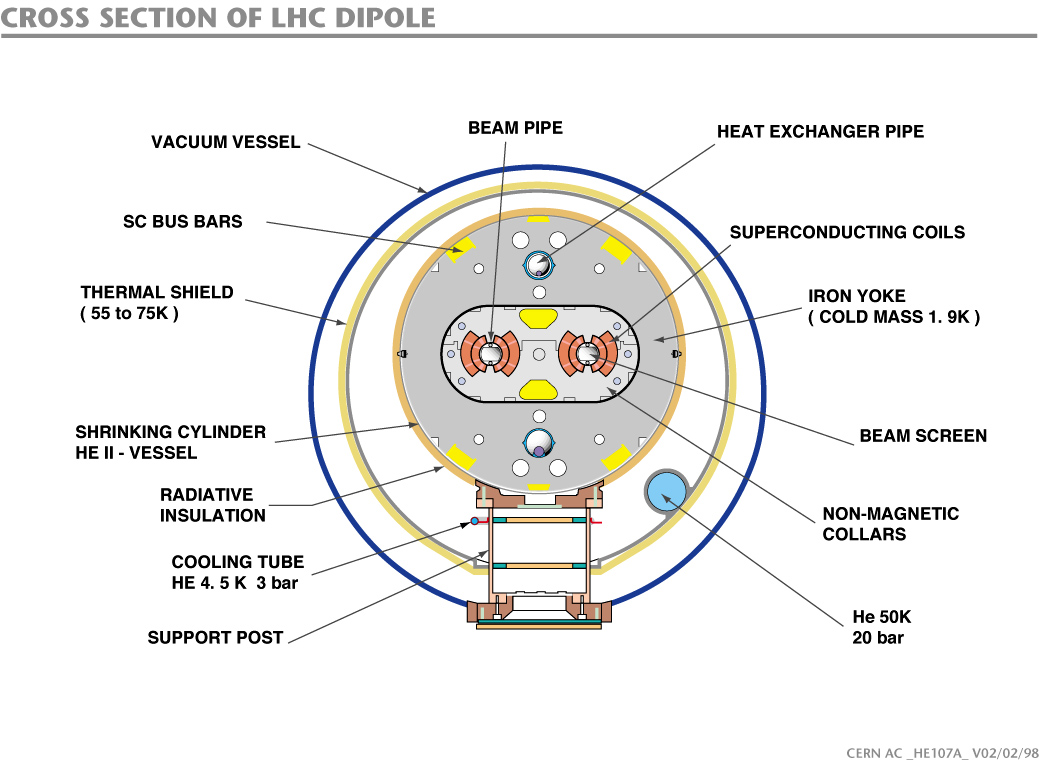
\includegraphics[width=.6\textwidth]{figures/LHC-magnets.jpg}
  \caption{Section of the LHC dipole magnet structure.}
  \label{fig:LHC_dipole}
\end{figure}

\noindent In fig.~\ref{fig:LHC_dipole}, a slice of the arc section is displayed. Around the beam pipes, two superconducting magnetic dipoles are located: they generate vertical magnetic fields in opposite directions. The superconducting coils are made of niobium-titanium, materials that are superconducting at very low temperature. At the LHC, they are kept at a temperature of 1.9 K (-$271.3^{\circ}$C) by a closed liquid helium circuit. A current of 11850 A flows through the magnets, without any energy loss due to electrical resistance, generating a magnetic field of 8.33 T. Magnets of higher order in multipole expansion (quadrupoles, sextupoles, octupoles, \textit{etc.}) are employed to optimize the proton trajectories; in particular, quadrupoles allow to focus and squeeze the beams. Along the LHC ring there are 9593 magnets; 1232 are dipoles, 392 are quadrupoles.

\begin{figure}[!htb]
  \centering
    %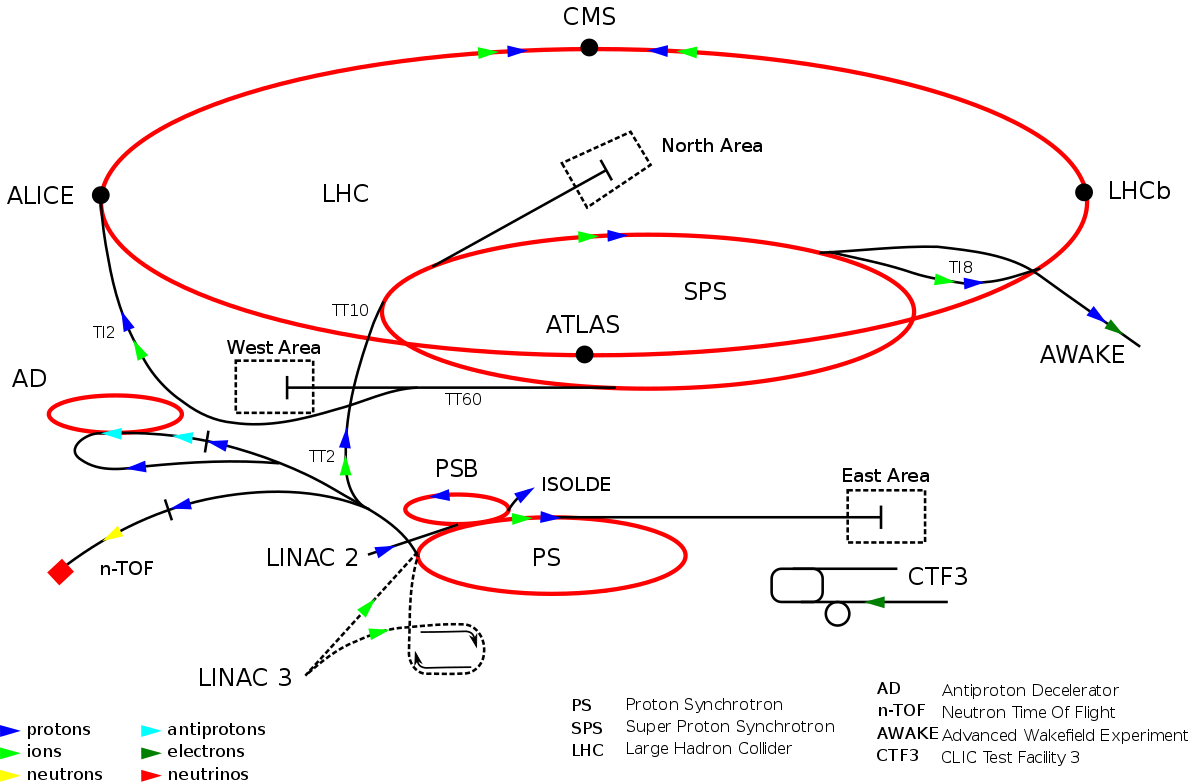
\includegraphics[width=.75\textwidth]{figures/Cern-accelerator-complex.png}\\
    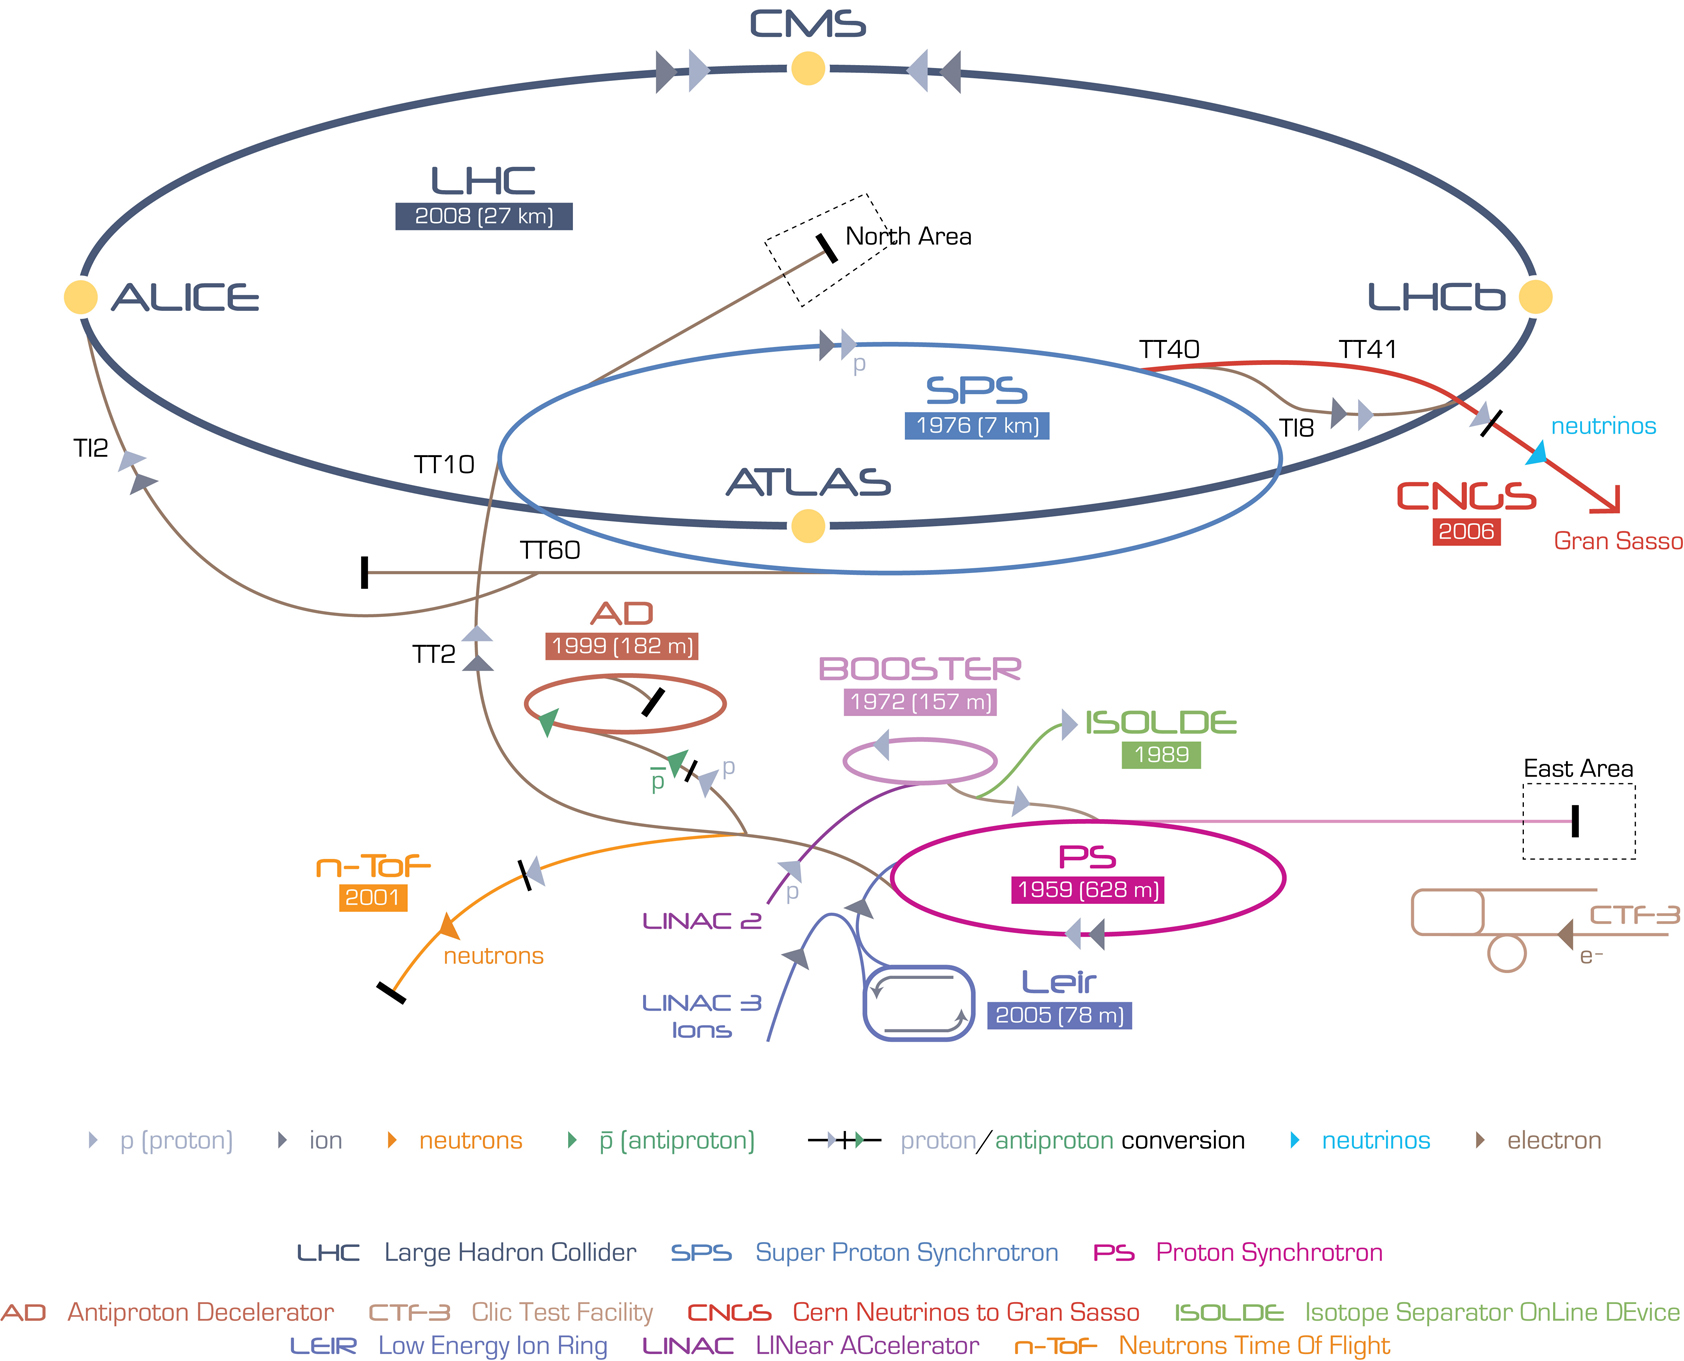
\includegraphics[width=.75\textwidth]{figures/Cern-Accelerator-Complex.jpg}
  \caption{The CERN accelerator complex.}
  \label{fig:LHC_accelerator_complex}
\end{figure}

\noindent The LHC represents the final step of the CERN accelerator complex, shown in fig.~\ref{fig:LHC_accelerator_complex}. Protons are extracted from hydrogen atoms and inserted in the linear accelerator Linac2, that brings them to an energy of 50 MeV. They circulate around a little synchrotron, the Proton Synchrotron Booster, reaching an energy of 1.4 GeV, and then in the Proton Synchrotron (PS), where their energy is increased to 25 GeV. The second to last step is the Super Proton Synchrotron, SPS, accelerating protons up to 450 GeV. They are finally injected in the Large Hadron Collider, where sixteen radiofrequency cavities (RF) accelerate protons inside each beam up to an energy of 6.5 TeV, corresponding to a center-of-mass energy of 13 TeV when colliding. The RF cavities provide an accelerating electromagnetic field up to 5 MV/m (maximum voltage of 2 MV), that oscillates with a frequency of 400 MHz. Like the magnets, the cavities are kept at low temperature (4.5 K, or -$268.7^{\circ}$C) in order to allow superconducting conditions. The maximum beam energy can be reached in 15 minutes. After several hours of collisions ($\sim 10$ hours), the quality of the beams deteriorates and they are extracted from the machine and dumped.\\

\noindent Protons circulate inside the LHC ring in bunches of $\sim10^{11}$ particles each, 80 mm long. Focusing magnets allow to reduce the bunch diameter down to 16 $\mu$m. Different bunches are separated by 25 ns (or, $\sim 7.5$ m), corresponding to a bunch collision frequency of 40 MHz and an instantaneous (peak) luminosity (defined in eq.~\ref{eq:LHC_luminosity_def}) of $1.2 \times 10^{34}\mbox{ cm}^{-2} \mbox{s}^{-1}$. Given the structure of the beams, at every bunch crossing many protons interact simultaneously: this phenomenon is called pile-up. The designed maximum number of bunches per fill is 2808.\\
%Protons with slightly different energies arriving earlier or later will be accelerated or decelerated so that they stay close to the energy of the ideal particle. In this way, the particle beam is sorted into discrete packets called "bunches". Top energy is reached in around 15 minutes, the bunches having passed the cavities around 1 million times.
%Queste frequenze elevate generano un problema noto con il nome di ``pile-up'', che consiste nel moltiplicarsi del numero di vertici primari di interazione. Ad un medesimo evento registrato prodotto dalle collisioni ogni 50 ns, infatti, corrispondono fino a 30 vertici di interazione; essi aumenteranno a 40 quando si arriver\`a a realizzare una collisione ogni 25 ns.\\

\begin{figure}[!htb]
  \centering
    \includegraphics[width=.5\textwidth]{PPD_results/int_lumi_per_day_cumulative_pp_2016.pdf}%
    \includegraphics[width=.5\textwidth]{PPD_results/int_lumi_per_day_cumulative_pp_2016_Golden_23Sep-PromEraH_Morion.png}

    \includegraphics[width=.5\textwidth]{PPD_results/int_lumi_per_day_pp_2016.pdf}%
    \includegraphics[width=.5\textwidth]{PPD_results/pileup_pp_2016.pdf}

  \caption{Luminosity in 2016 LHC data. Top-left plot: the cumulative integrated luminosity delivered by the LHC (in blue) and recorded by the CMS detector (in orange), as a function of the data-taking period. Top-right plot: data recorded by CMS and declared as optimal for the physics analyses (in light orange), corresponding to a total integrated luminosity of 35.9 $\text{fb}^{-1}$. Bottom-left plot: maximum integrated luminosity per day. Bottom-right plot: number of proton interactions per bunch crossing (pile-up).}
  \label{fig:LHC_lumi}
\end{figure}

\noindent The main parameters characterizing an hadronic collider are the center-of-mass energy, corresponding to the sum of the energies of the beams, and the instantaneous luminosity, that describes the frequency of the interactions among the bunches in the beams. If the bunches in the first beam contain $n_1$ protons, the bunches in the second beam contain $n_2$ protons, the colliding area is $\Sigma$, and the frequency of complete turns
around the ring is $f$, the instantaneous luminosity $\mathcal{L_{\text{inst}}}$ is:

\begin{equation}
\mathcal{L_{\text{inst}}} = f \frac{n_1 n_2}{\Sigma}.
\label{eq:LHC_luminosity_def}
\end{equation}

\noindent If a generic physics process $i$ has a cross-section of $\sigma_i$, the interaction rate $R_i$ is:
\begin{equation}
R_i = \frac{dN_i}{dt}= \sigma_i \mathcal{L_{\text{inst}}};
\label{eq:LHC_interaction_rate}
\end{equation}
the number of events $N_i$ recorded in the time interval $(0,\tau)$ is obtained from the integrated luminosity $\mathcal{L} = \int_0^{\tau} \mathcal{L_{\text{inst}}} dt$:
\begin{equation}
N_i = \sigma_i \int_0^{\tau} \mathcal{L_{\text{inst}}} dt.
\end{equation}

\noindent In fig.~\ref{fig:LHC_lumi}, a summary of the luminosity measurements in 2016 data is presented. The luminosity delivered by the LHC is represented in blue, the luminosity recorded by the CMS is displayed in orange. The mean number of interactions per bunch crossing (pile-up) is presented as well. The average number of interactions per collision is 27, the maximum is generally around 50 (in fig.~\ref{fig:pp_pileup}, a record of 78 pile-up collisions was detected).

\begin{figure}[!htb]
  \centering
    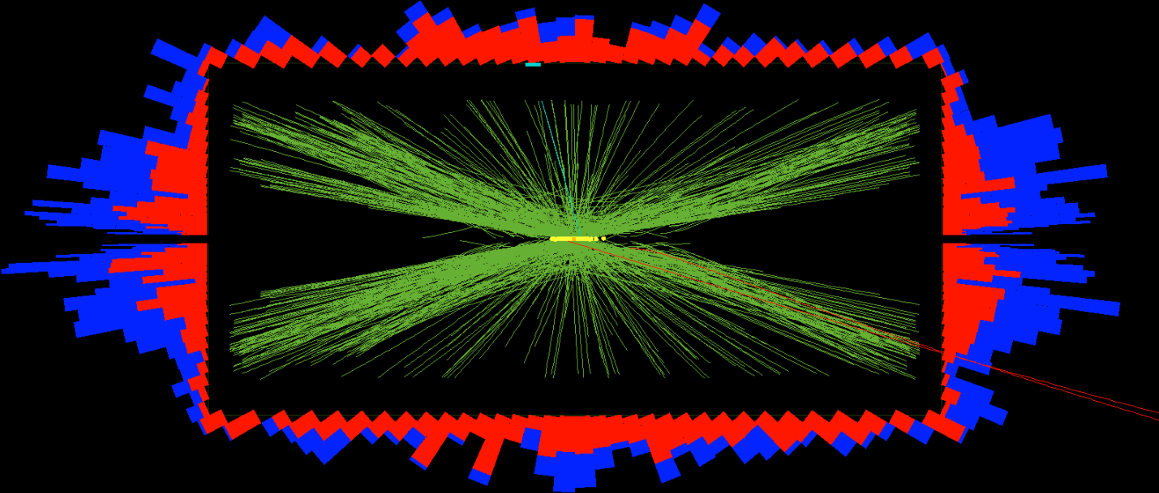
\includegraphics[width=.5\textwidth]{figures/78events_PU_b.png}
  \caption{CMS collision event, where a record of 78 interactions per single bunch crossing were taking place simultaneously.}
  \label{fig:pp_pileup}
\end{figure}

\subsection{Proton-proton interactions}
%Figura da CMS Collaboration, DAQ generic figures gallery online at http://cmsdoc.cern.ch/cms/TDR/DAQ/TDRweb/daqgenericjpg.htm
\noindent Proton-proton collisions allow to reach high energies and luminosities, but the drawback is the complexity of the events when compared to electron-positron collisions: not only because of the increasing backgrounds due to strong interaction among partons, but also because the momenta of the proton partons taking part in the interaction are unknown; not to mention the problem of disentangling the tracks of the particles coming from the interesting hard interactions from the spectator pile-up interactions.\\
The majority of the LHC events is represented by soft interactions, with low transverse momentum transfer, namely elastic and diffractive scatterings. In the so-called hard interactions, on the other hand, the transferred momentum among particles is high, allowing to produce massive resonant phenomena. These events manifest in peculiar final state signatures that can be distinguished from the soft background interactions.\\
At high momentum transfer (perturbative regime), a proton can be described as a collection of partons, each bringing a fraction $x$ of the initial beam momentum, whose distributions are described by the parton distribution functions (PDF), $f(x,Q^2)$, as a function of the Bjorken's variable $x$ and of the momentum transfer $Q^2$. At very high center-of-mass energies (13 TeV), the proton mass can be neglected; the available energy in the parton 1 -- parton 2 scattering is unknown, $\sqrt{x_1 x_2 s}$. The total cross-section of any interaction is given by:
\begin{equation}
\sigma = \int dx_1 f_1(x_1,Q^2) \int dx_2 f_2(x_2,Q^2) \sigma_{12}(x_1 p_1, x_2 p_2, Q^2),
\end{equation}
where $\sigma_{12}$ is the cross-section at parton level, and $f_1,f_2$ are the parton PDFs. In fig.~\ref{fig:LHC_pp_cross_section}, parton cross-sections of the main standard model processes are displayed, as a function of the center-of-mass energy.

\begin{figure}[!htb]
  \centering
    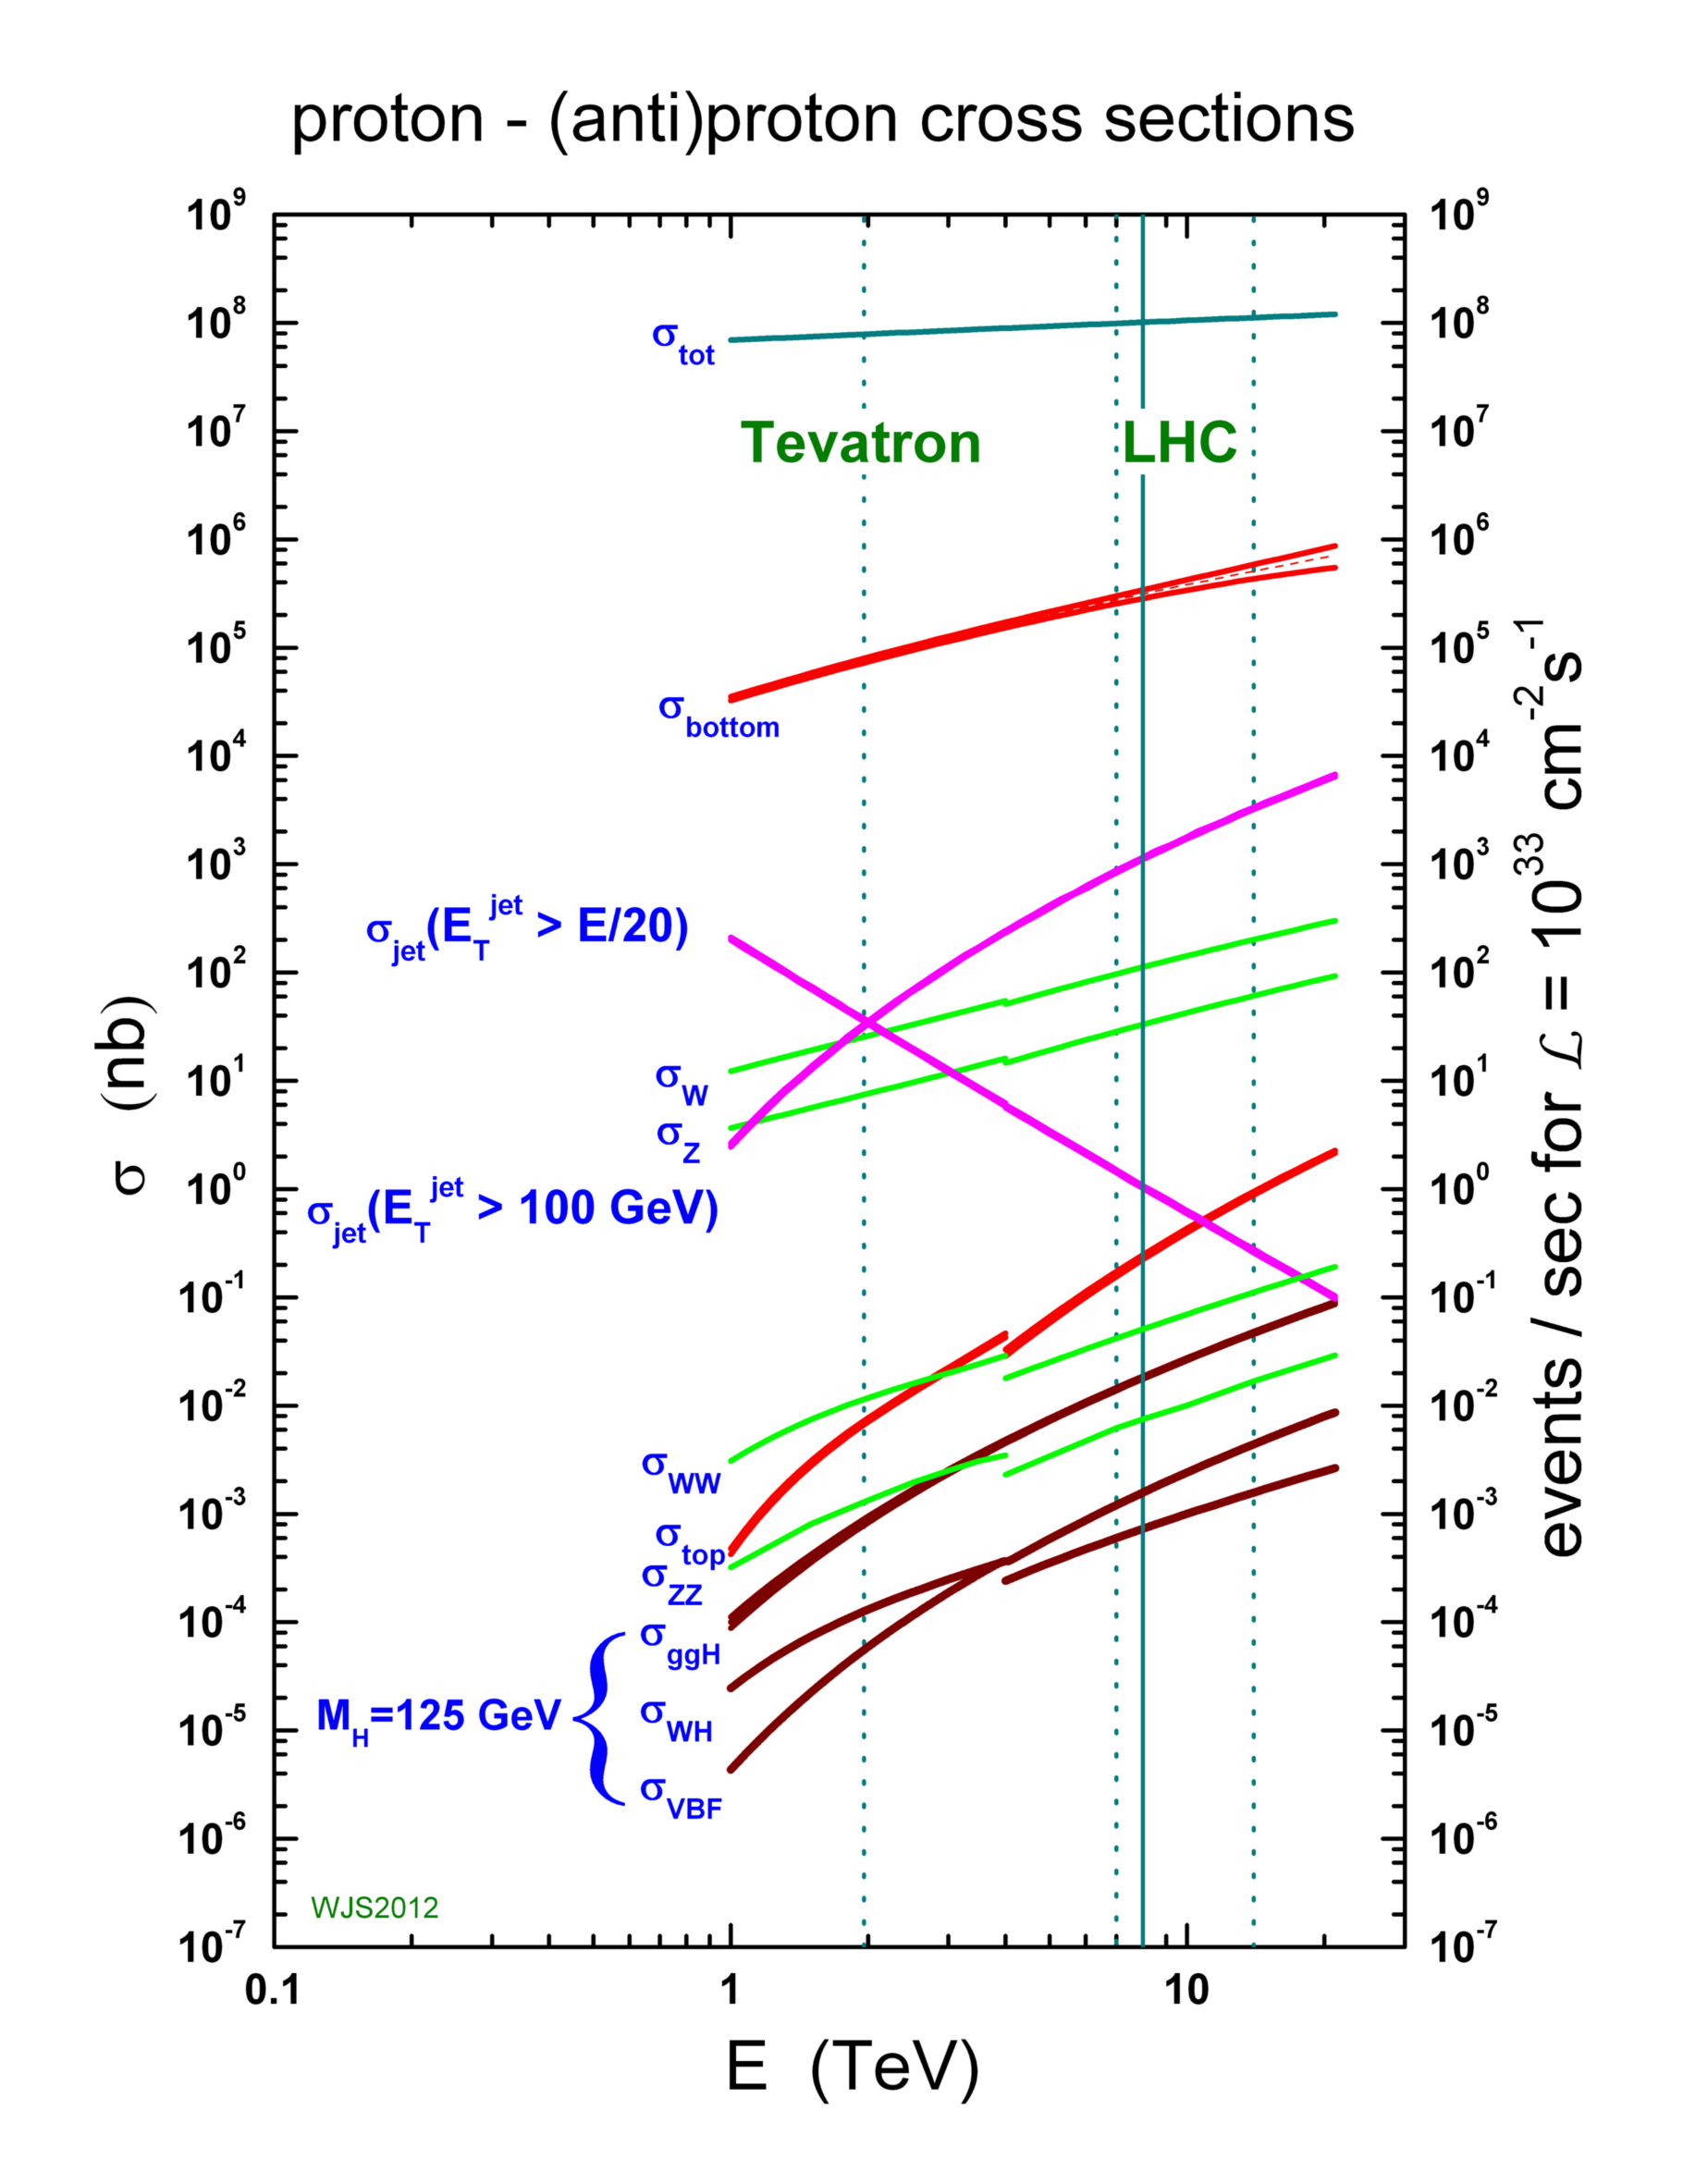
\includegraphics[width=.5\textwidth]{figures/crosssections2013.jpg}
  \caption{Cross-sections and number of expected events in proton-proton collisions, as a function of the center-of-mass energy. Rare phenomena, such as the Higgs boson production, can be observed at the LHC.}
  \label{fig:LHC_pp_cross_section}
\end{figure}

\section{The CMS detector}

The Compact Muon Solenoid (CMS) is a multi-purpose detector built in the LHC ring. It is situated in a cavern 100 m underground, near Cessy, in France. It is a cylinder 22 m long, with a diameter of 15 m, and a weight of 12500 tons. Its physics programme includes the search for the Higgs boson (discovered in 2012), precision measurements of the standard model parameters and rare decays (physics of bottom quark), and search for new physics beyond the SM (SUSY, exotic phenomena, dark matter, extra dimensions).\\
The CMS detector is structured in many layers of sub-detectors, giving different responses depending on the nature and the momentum of the particles passing through. The inner detectors have been finely segmented in order to afford the high radiation levels and particle multiplicity at the interaction point, so that the reduced occupancy of each layer allows to measure and distinguish precisely the primary vertices of the hard interactions from the pile-up events. A very accurate time resolution is necessary to synchronize all the subsystems together.\\
%La maggior parte dei processi fisici che si vogliono esplorare hanno basse sezioni d'urto, mentre, come \`e ben noto, i prodotti delle collisioni tra protoni sono dominati da elevati fondi QCD: CMS \`e progettato in modo da avere un'elevata capacit\`a di discriminazione degli eventi rari, sfruttando in particolare i canali comprendenti elettroni e muoni, e una grande precisione di misura dei vertici secondari, necessaria per distinguere i $\tau$ e gli adroni contenenti quark pesanti. L'elevata luminosit\`a nominale di LHC, come accennato, comporta il problema del pile-up: questi effetti possono essere ridotti utilizzando rivelatori ad elevata granularit\`a. L'occupazione si abbassa segmentando l'apparato in molti sottogruppi di rivelatori, al costo di dover ottenere un'ottima sincronizzazione tra di essi. L'alta frequenza di interazione, inoltre, necessita un'alta risoluzione temporale. Infine, gli elevati livelli di radiazione attorno al vertice richiedono apparati robusti e resistenti.

\begin{figure}[!htb]
  \centering
    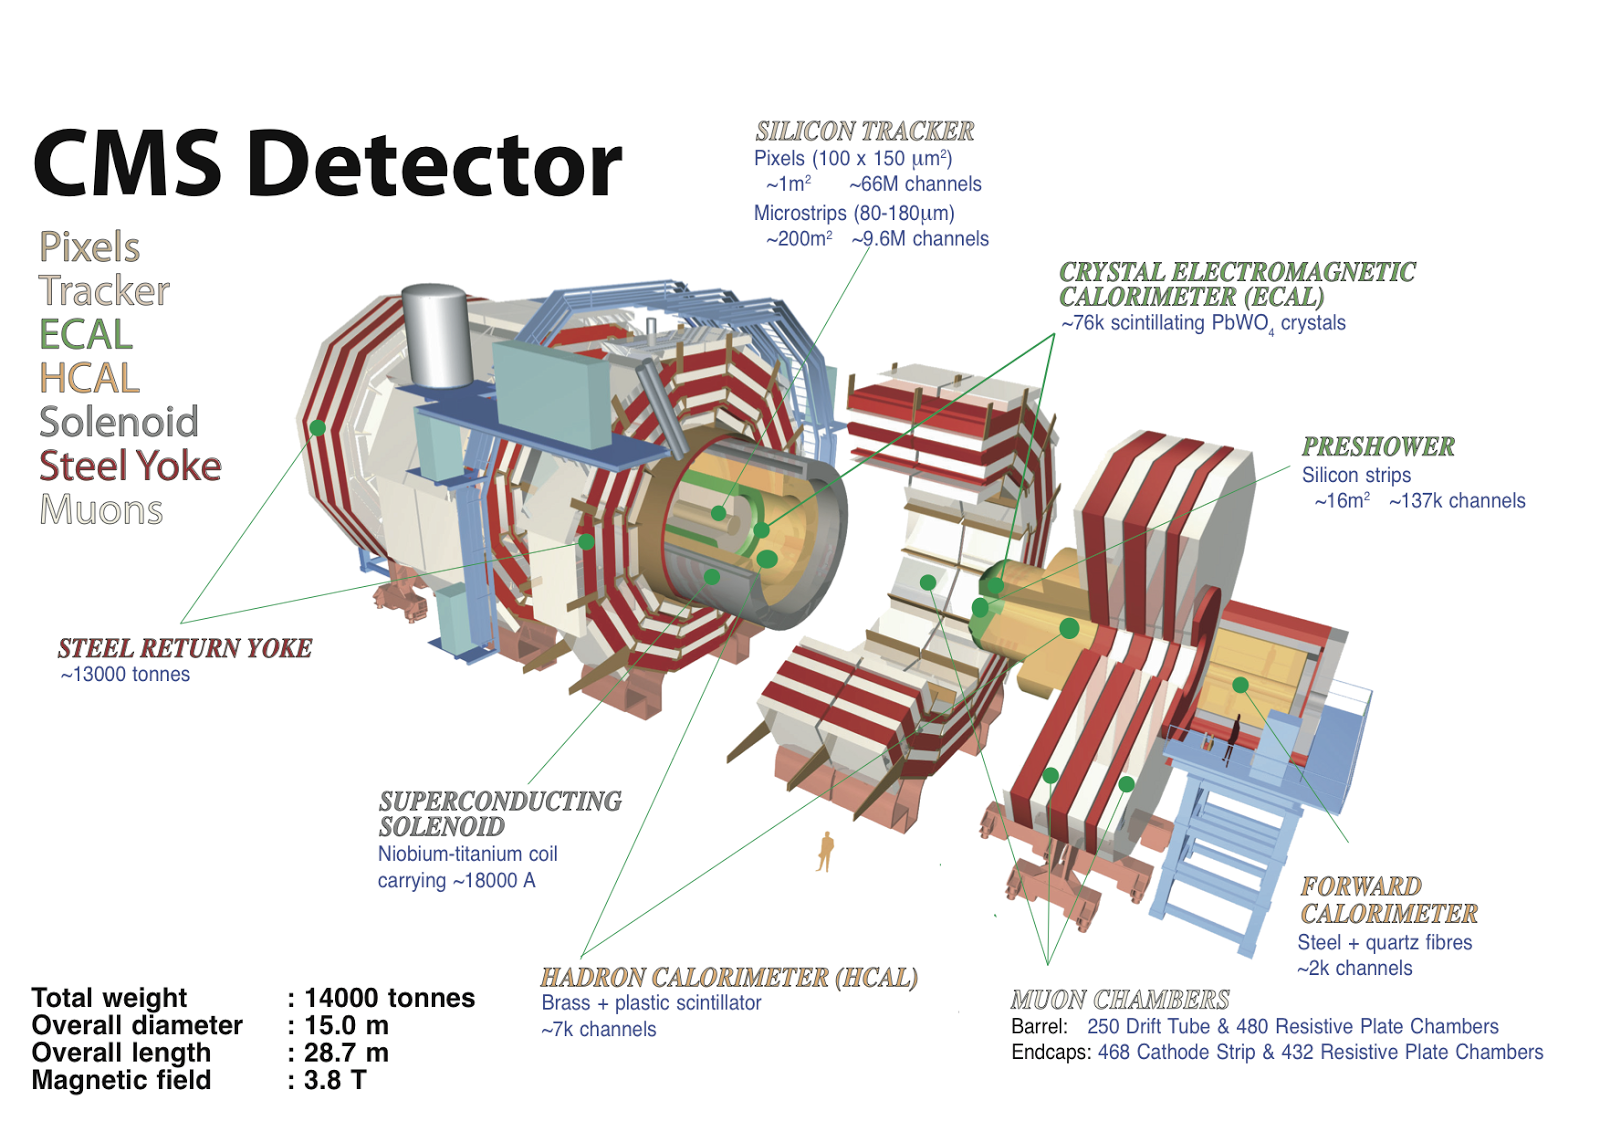
\includegraphics[width=.99\textwidth]{figures/cms_3d.png}
  \caption{The CMS experiment.}
  \label{fig:CMS_1}
\end{figure}

\noindent Fig.~\ref{fig:CMS_1} shows a sketch of the CMS detector. It is longitudinally segmented in the barrel region and two endcaps. In the forward region (over the endcaps), where the beam radiation is very intense, additional calorimeters have been placed. In fig.~\ref{fig:CMS_particles}, the mean path of a specific particle through the sub-detectors is represented, depending on its flavour.\\
A detailed description of the CMS detector can be found in~\cite{Chatrchyan:2008zzk}.

\begin{figure}[!htb]
  \centering
    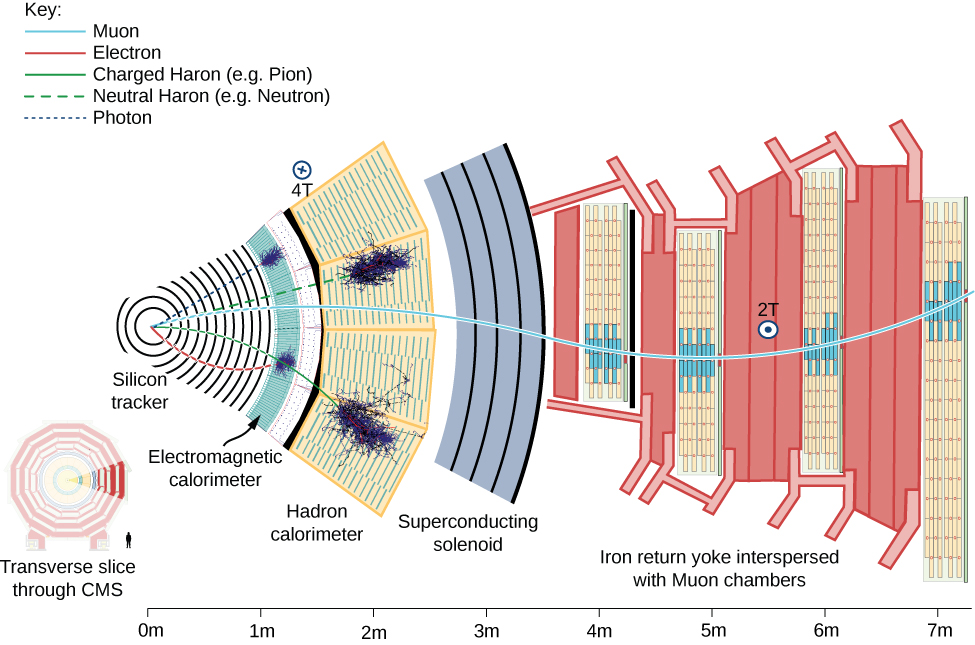
\includegraphics[width=.99\textwidth]{figures/CMS_particles.jpg}
  \caption{Mean path of a particle through the CMS detector. A muon, in light blue, passes through with a bended trajectory, depending on its momentum and charge, triggering signals in all the sub-systems. An electron, in red, leaves a track in the silicon tracker and is absorbed by the electromagnetic calorimeter. A neutral or charged hadron, in green, stops inside the hadronic calorimeter. A photon, dotted blue line, showers in the electromagnetic calorimeter, without leaving any track in the silicon detector.}
  \label{fig:CMS_particles}
\end{figure}

\subsection{The coordinate system}
\label{ssec:coord_syst}
The CMS coordinate system is depicted in fig.~\ref{fig:CMS_CoordSys}. $x$ and $y$ are the coordinates in the transverse plane, $z$ is the longitudinal coordinate. The $x$ axis points at the center of the LHC ring, the $y$ axis points upward, the $z$ axis is along the beam direction. The azimuthal angle $\varphi$ lies in the transverse plane, and it is measured starting from the $x$ axis; the radial coordinate is $r$. The polar angle $\theta$ lies in the plane $(r,z)$. The transverse component of the 3-momentum, $\vec{p}_T$, is orthogonal to the beam axis and lies in the plane $(x,y)$. The transverse energy is defined as the magnitude of $\vec{p}_T$: $E_T = E \sin{\theta}$.\\
Two other commonly used variables are the rapidity, \rap, and pseudorapidity, $\eta$, defined as functions of the particle energy $E$, the longitudinal component of the momentum $p_z$ and the 3-momentum modulus:
\begin{equation}
\begin{split}
 & \rap = \frac{1}{2} \log{\frac{E + p_z}{E - p_z}}\\
 & \eta = \frac{1}{2} \log{\frac{|\vec{p}| + p_z}{|\vec{p}| - p_z}} = -\log{\tan{\frac{\theta}{2}}}.
\end{split}
\end{equation}
When the considered particle is produced in the forward region, hence at $\theta = 0$, it means that $\eta~\rightarrow~\infty$. When the particle is produced in the transverse plane, hence $\theta = \pi /2$, $\eta = 0$. At high energies, when the masses can be neglected, rapidity and pseudorapidity coincide; these variables are largely used at colliders because they are invariant under Lorentz boosts along the beam direction.

\begin{figure}[!htb]
  \centering
    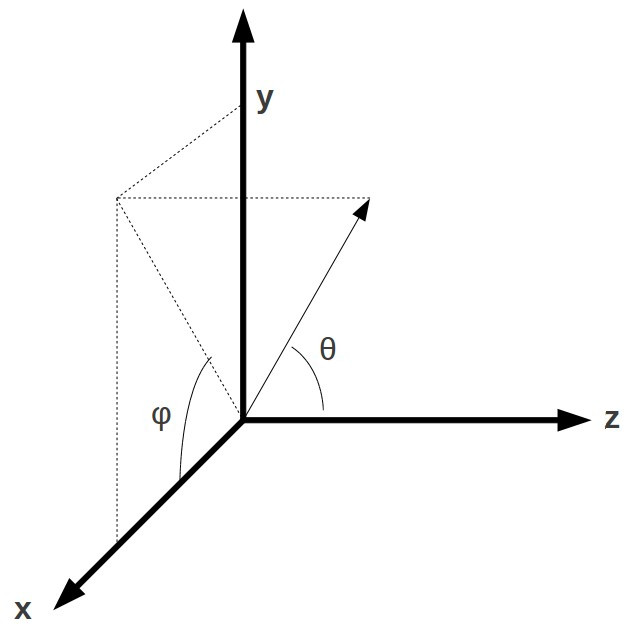
\includegraphics[width=.25\textwidth]{figures/CMS_CoordSys.jpg}
  \caption{The CMS coordinate system.}
  \label{fig:CMS_CoordSys}
\end{figure}

\subsection{The magnet}
The CMS superconducting magnet is an hollow cylinder (13 m long, 6 m of diameter, shown in fig.~\ref{fig:CMS_solenoid}). An electrical current of 19 kA flows through the niobium and titanium fibers that constitute the solenoid, providing a maximum magnetic field of 3.8 T and storing a maximum energy of 2.6 GJ. Superconducting conditions are mantained by a liquid helium cooling system, keeping the solenoid temperature at 4.5 K. In order to avoid stray fields, the magnetic field lines are closed by the return yoke, composed by 10 ktons of magnetized iron blocks, located in the outer part of CMS and alternated to the muon chambers. The homogeneus magnetic field inside the detector bends the trajectories of the charged particles, allowing the measurement of their momenta $p$, given the relation with the magnetic field strength $B$ and the radial coordinate $r$ of the trajectory:
\begin{equation}
p [\text{GeV}] = 0.3 \times B [\text{T}] \times r [\text{m}]. 
\end{equation}

\begin{figure}[!htb]
  \centering
    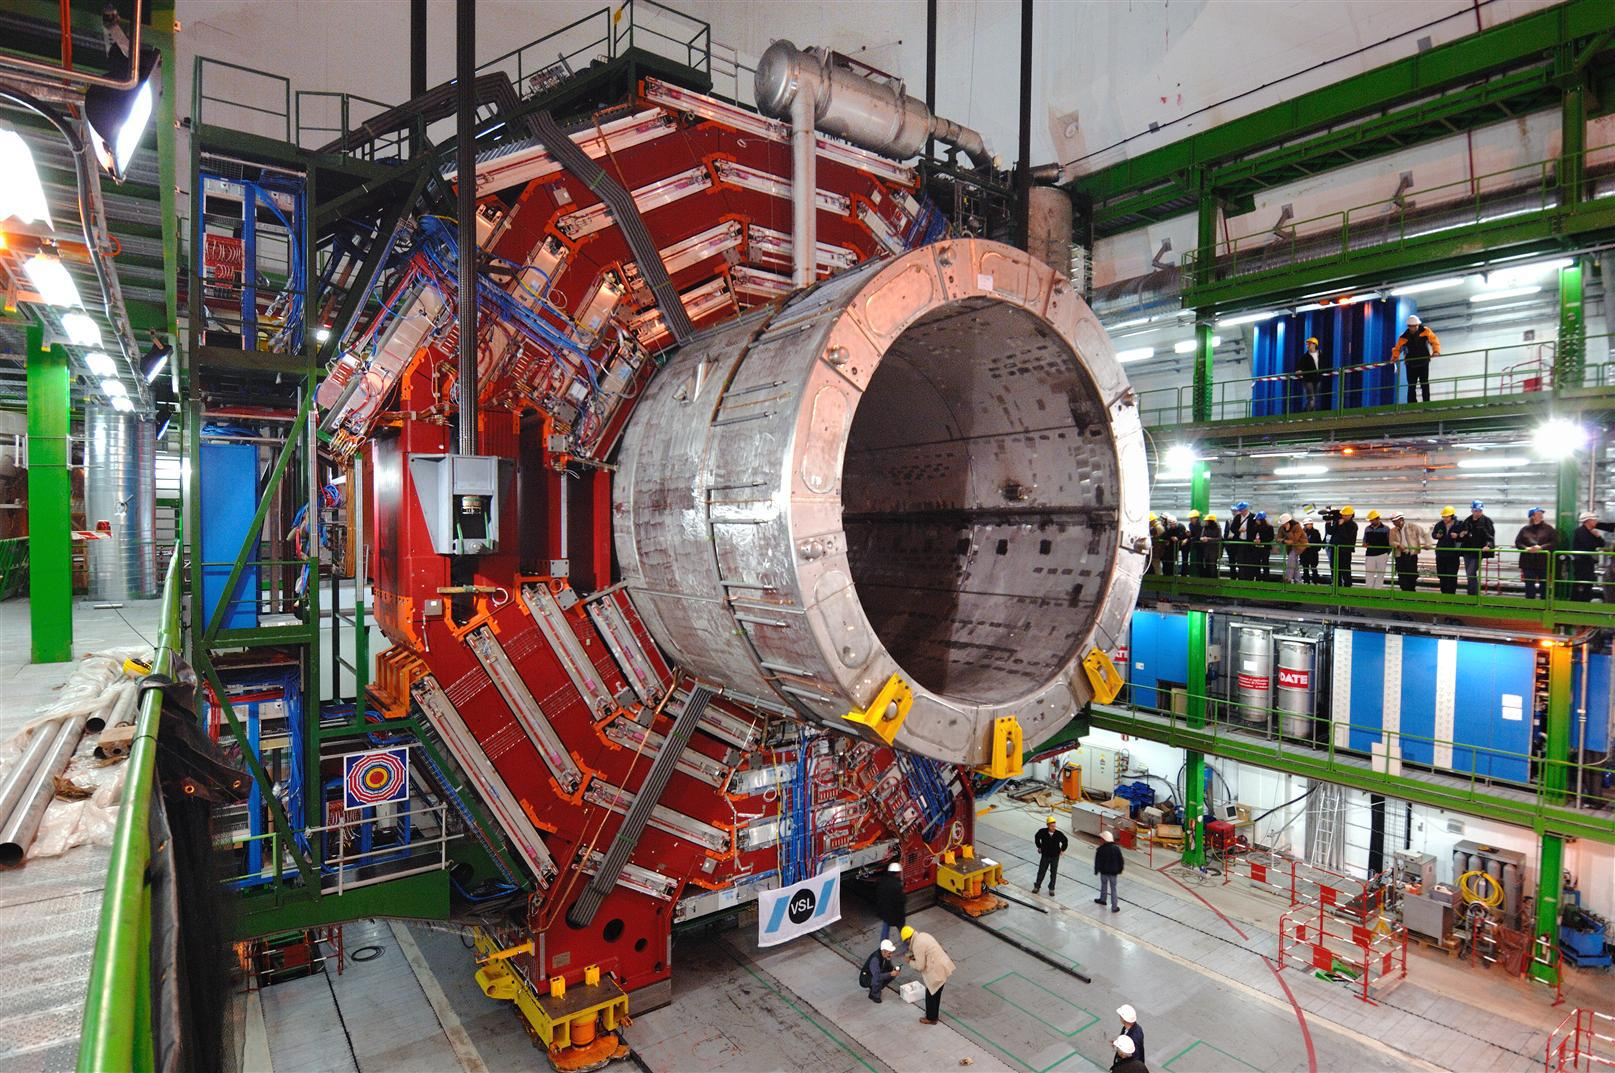
\includegraphics[width=.5\textwidth]{figures/CMS_solenoid.jpeg}
  \caption{Installation of the superconducting solenoid in the CMS cavern.}
  \label{fig:CMS_solenoid}
\end{figure}

\subsection{The tracking system}
\begin{figure}[!htb]
  \centering
    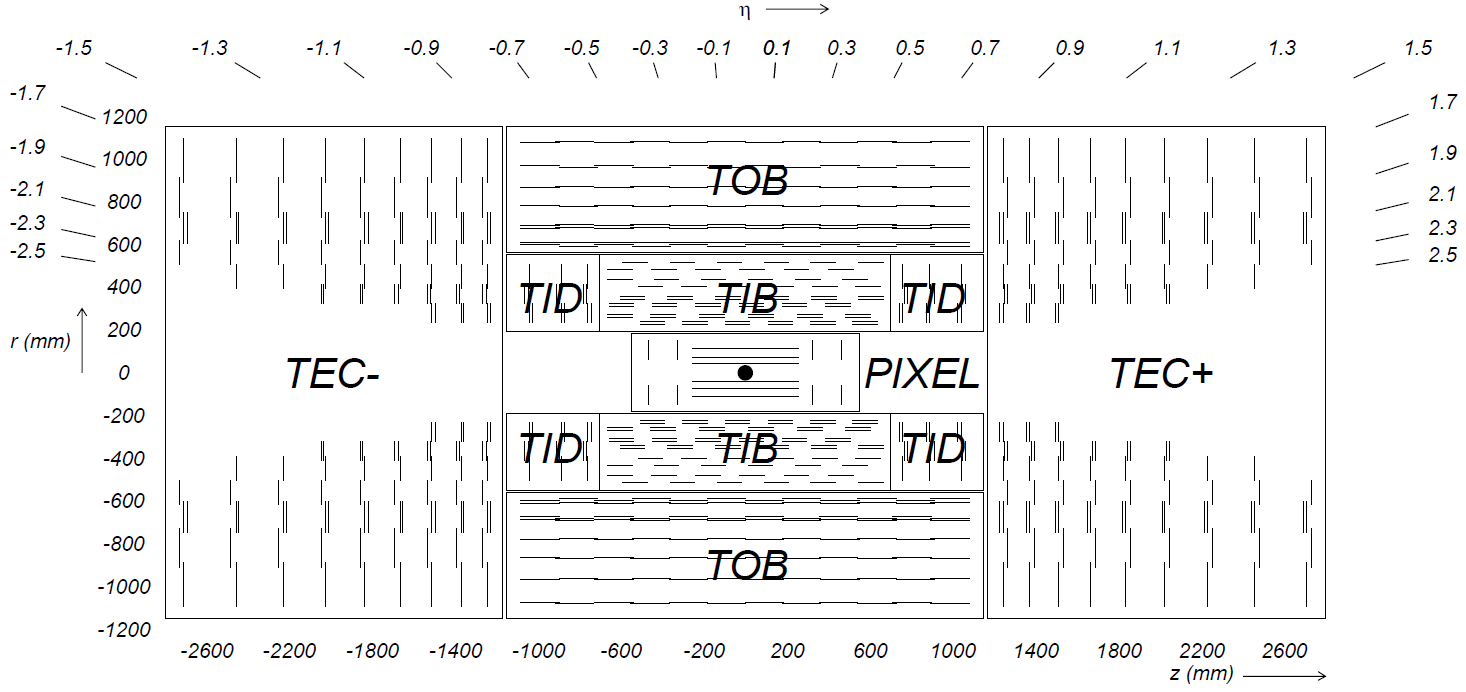
\includegraphics[width=.9\textwidth]{figures/cmstracker.png}
  \caption{The CMS tracking system: the inner pixel detector, close to the interaction point, and the outer strip detector.}
  \label{fig:CMS_tracker}
\end{figure}

The CMS tracking system~\cite{Karimäki:368412,Chatrchyan:2014fea} is composed by a cylinder of silicon detectors (2.5 m of diameter and 5.8 m of length). Their design guarantees a precise reconstruction of the tracks left by charged particles and of the interaction vertices, a fundamental tool to identify heavy quarks (charm, beauty) and leptons (taus).
Tracker detectors cover a pseudorapidity region of $|\eta|<2.5$ and have an active area of $210\text{ m}^2$. The two sub-detectors of the tracking system are the pixel detector, installed close to the interaction point, and the strip detector, covering a radius of 0.2 -- 1.2 m. The high granularity of the pixels and strips allows to keep the occupancy at acceptable levels, given the high multiplicity of the tracks ($\sim$1 MHz/$\text{mm}^2$). The silicon detectors and the electronic cables are cooled down to a temperature of $\sim 10^{\circ}$ C. The structure of the tracking system is shown in fig.~\ref{fig:CMS_tracker}.

\subsubsection{The pixel detector}
The pixel detector is composed by 66 millions of silicon cells, whose dimensions are $100 \times 150 \text{ }{\mu{m}}^2$, 285 $\mu$m of thickness, placed in 1440 modules. Silicon cells are set in three layers in the barrel region and in two disks at each endcap. Barrel modules are disposed parallel to the magnetic filed, whilst at the endcap they are tilted by about $20^{\circ}$. 
%Il pixel detector \`e costituito da tre strati di rivelatori nel barrel e da due dischi agli endcaps. I moduli nel barrel sono disposti parallelamente al campo magnetico, mentre agli endcaps sono inclinati di circa $20^{\circ}$: le coppie elettrone-lacuna prodotte nel semiconduttore sono allora soggette ad una forza di Lorentz e il loro moto di deriva non avviene pi\`u lungo le linee del campo elettrico, bens\`i esse si sparpagliano lungo diversi pixel. Calcolando il centro della distribuzione di carica raccolta, \`e possibile determinare la posizione della particella carica che ha attraversato il rivelatore con una risoluzione di 15 $\mu$m, sia nel piano $\mathrm{r}\Phi$, sia lungo $\mathrm{z}$.\\
Pixels allow a spatial resolution of 10 $\mu$m in the transverse plane, and of $\sim$20 $\mu$m along the longitudinal coordinate. Their reduced size guarantees an occupancy of $10^{-4}$ per pixel at each bunch crossing, in high luminosity regime.

\subsubsection{The strip detector}
The strip system is divided in the four-layered tracker inner barrel (TIB), covering a region $20 < r < 55$ cm with respect to the interaction point, the six-layered tracker outer barrel (TOB), located at $55 < r < 110$ cm, the three tracker inner disks (TID) and the nine tracker endcaps (TEC) at each cylinder base. Given the lower radiation level at higher radii (and hence a lower occupancy, around few percent), strips are bigger than pixels. Silicon strips in TIB and TID are 320 $\mu$m thick, 10 cm long, and with a pitch ranging from 80 to 120 $\mu$m; strips in TOB and TEC are 25 cm long, with a different thickness (320 $\mu$m for TID, 500 $\mu$m for TEC) and pitch (97-184 $\mu$m). There are 15148 strip modules, and 9.3 million readout channels. The strip spatial resolution is about 20 -- 50 $\mu$m in the transverse plane and about 200 -- 500 $\mu$m along the longitudinal coordinate.
%Nel capitolo 4 descriver\`o le tecniche di ricostruzione delle tracce nei rivelatori al silicio, in particolare dei muoni.\\
%L'efficienza di ricostruzione delle tracce dei muoni \`e stata misurata essere attorno al 99\%, essa cala drasticamente per $|\eta|>2.1$ a causa della ridotta copertura geometrica del pixel detector. Le efficienze di rivelazione degli adroni sono tipicamente pi\`u basse perch\'e interagiscono con il materiale. La risoluzione in $p_T$, sempre per i muoni, \`e attorno all'1-2\% per $|\eta|>1.6$ e per momenti elevati; a momenti pi\`u bassi dominano effetti di scattering multiplo e dipendono dalla quantit\`a di materiale attraversato.\\

\subsection{The electromagnetic calorimeter}
The CMS electromagnetic calorimeter (ECAL, shown in fig.~\ref{fig:CMS_ecal})~\cite{ECAL-TDR} is a homogeneous detector composed by lead tungstate ($\text{PbWO}_4$) scintillating crystals, designed to measure the energy deposits of photons and electrons through their electromagnetic showers. $\text{PbWO}_4$ is transparent and dense (8.3 gr/$\text{cm}^3$); it has a fast time response (the 85\% of the scintillating light is emitted at every bunch crossing), high scintillating efficiency and radiation resistance; it has a radiation length of $X_0~=~0.89$~cm and a Moli\`ere radius of 2.19~cm. The ECAL is divided in the barrel region ($\eta < 1.479$, at a radius of 1.3 m) and the endcaps ($1.479 < \eta < 3$).  The 61200 crystals employed in the barrel region, whose size is $(22 \times 22) \text{ mm}^2 \times 23 \text{ cm}$, have a radiation length of $25.8 X_0$; the 7324 crystals in the endcaps, of size $ 28.6 \times 28.6 \text{ mm}^2 \times 22 \text{ cm}$, have a radiation length of $24.7 X_0$. Before the endcaps, on each side, a pre-shower detector is installed: it is composed by two disks of lead absorber and two layers of silicon strips, of radiation lengths up to $3X_0$. The pre-shower calorimeter has been designed to distinguish the photons coming from the $\pi^0$ decay, from the photons produced in the rare Higgs decay $H \rightarrow \gamma \gamma$. The readout and amplification of the scintillating light, performed by avalanche photodiodes in the barrel and by vacuum phototriodes in the endcaps, requires a stable temperature of $18^{\circ}$ C, mantained by a water cooling system.

\begin{figure}[!htb]
  \centering
    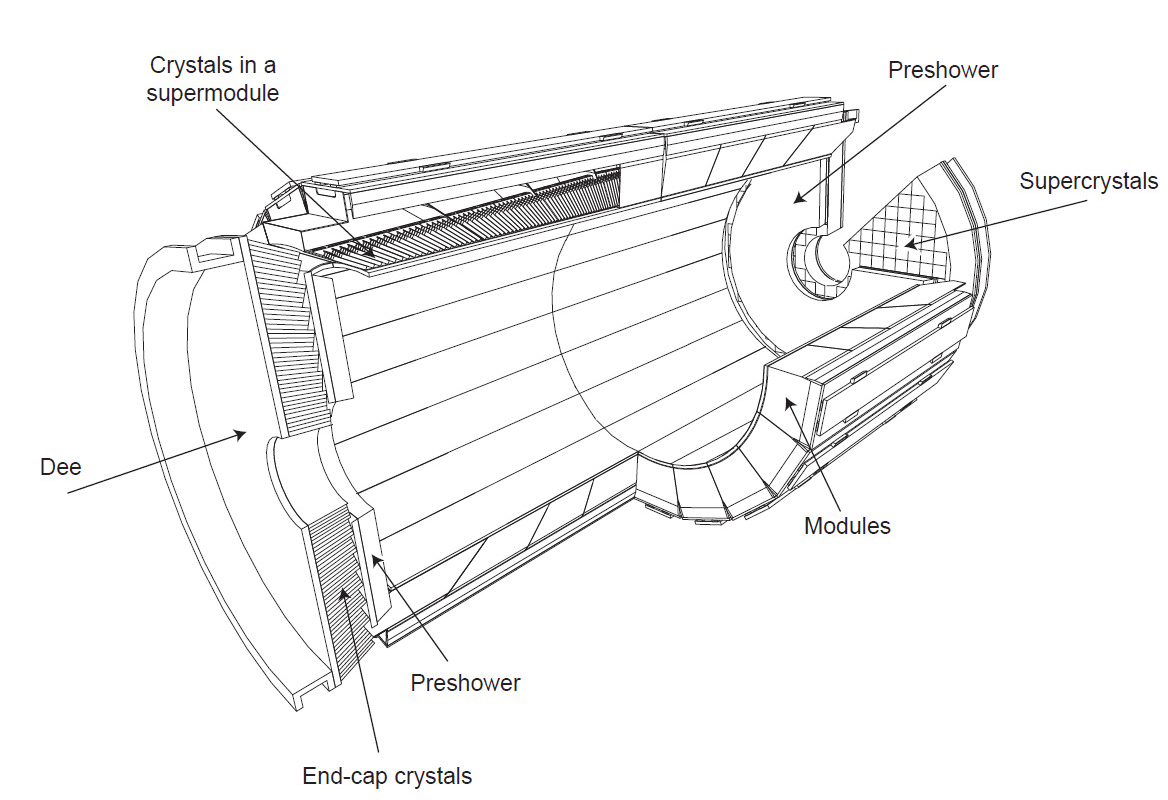
\includegraphics[width=.7\textwidth]{figures/cmsecal.png}
  \caption{The CMS electromagnetic calorimeter.}
  \label{fig:CMS_ecal}
\end{figure}

%\begin{figure}%{l}{0.5\textwidth}
%\centering
%%\includegraphics[scale=0.3]{risoluzione_ECAL.png}
%\caption{Risoluzione in energia di ECAL in funzione dell'energia del fascio di elettroni utilizzato per le misure. Sono mostrati anche i valori per i parametri di fit[16].}
%\label{fig:risoluzione_ECAL}
%\end{figure}
\noindent The energy resolution of the calorimeter is parametrized as:
\begin{equation}
{\left( \frac{\sigma}{E} \right)}^2 = {\left( \frac{S}{\sqrt{E}} \right)}^2 + {\left( \frac{N}{E} \right)}^2 + C^2,
\end{equation}
where $S=0.018 \text{ GeV}^{\frac{1}{2}}$ is the stochastic term, $N=0.04$ GeV is related to noise contribution, and $C=0.005$ is a constant term depending on the calibration.
%In figura \ref{fig:risoluzione_ECAL} sono mostrati i risultati ottenuti da misure di prova con un fascio di elettroni: le stime ottenute sono $S=0.028 \mbox{ GeV}^{\frac{1}{2}}$, $N=0.12 GeV$, $C=0.003$.


\subsection{The hadronic calorimeter}
The hadronic calorimeter (HCAL, displayed in fig.~\ref{fig:CMS_hcal})~\cite{HCAL-TDR} is a sampling calorimeter, composed of brass and plastic scintillator layers. It has been designed to guarantee a good hermeticity, allowing to perform a precise measurement of the missing transverse energy. It is located within the electromagnetic calorimeter and the solenoid, covering a region of $|\eta|<1.3$ in the barrel, and $1.3<|\eta|<3$ in the endcaps. Brass is non-magnetic and has short interaction length (16.4 cm): the 60 mm thick absorber layers used in the barrel reach 5.6 interaction lengths at $\eta=0$ and 10.8 interaction lengths at $\eta = 1.3$; the 80 mm thick layers in the endcaps reach 11 interaction lengths. An additional calorimetric layer has been installed out of the solenoid, in order to reach 11.8 interaction lengths in the barrel region. The scintillation light, typically in the blue-violet region of the electromagnetic spectrum, is collected by wavelength-shifter fibers, translated and amplified by multi-channel hybrid photodiodes, proportionally to the magnitude of the energy deposits. An additional hadronic calorimeter (HF) has been placed in the forward region, $3 < |\eta| < 5.2$, at 11.2 m from the interaction point. It has beeen studied to afford the high levels of radiation: it is composed by 55 mm thick absorber layers of stainless-steel, and quartz fibers, able to detect the Cherenkov scintillating light of the charged particles of the hadronic showering. A longitudinally segmentation allow to distinguish hadronic particles from electromagnetic components.
The energy resolution of the hadronic calorimeter is:
\begin{equation}
\left( \frac{\sigma}{E} \right) \approx \frac{a}{\sqrt{E}} \oplus b\%,
\end{equation}
where $a=65\%$ in the barrel region, $85\%$ in the endcaps, $100\%$ in the forward region, and $b=5\%$.

\begin{figure}[!htb]
  \centering
    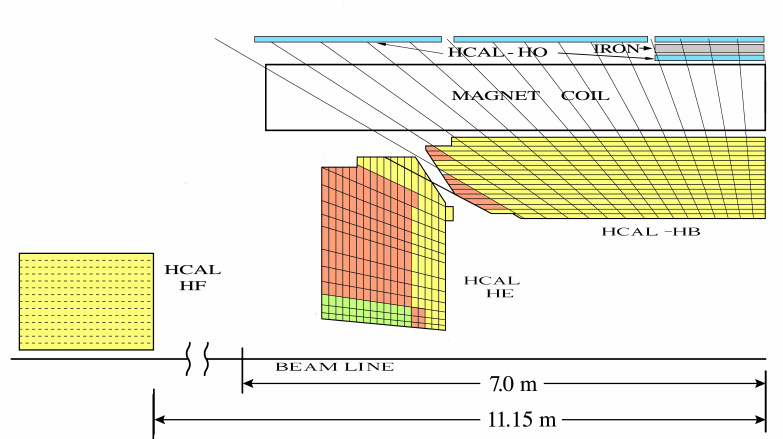
\includegraphics[width=.7\textwidth]{figures/cmshcal.png}
  \caption{The CMS hadronic calorimeter.}
  \label{fig:CMS_hcal}
\end{figure}


\subsection{The muon system}


The outer system of the CMS experiment consists into gas detectors for identifying muons~\cite{MUON-TDR}, that are located between the iron return yokes, designed to close the magnetic field generated by the solenoid. In the barrel region, where a smaller number of muons is expected and the magnetic field is less strong, Drift Tubes (DT) detectors are installed. In the endcaps, where the flux of particles is larger, Cathod Strip Chambers (CSC) are used, and disposed in three disks. CSCs are designed to allow faster responses, higher granularity and radiation resistance. Resistive Plate Chambers (RPC) are installed both in the barrel and in the endcaps as additional triggering system. The geometry of the muon system is shown in fig.~\ref{fig:CMS_muon}; it consists of 250 DTs, 530 CSCs, 610 RPCs, and it covers a region $|\eta|<2.4$.

\begin{figure}[!htb]
  \centering
    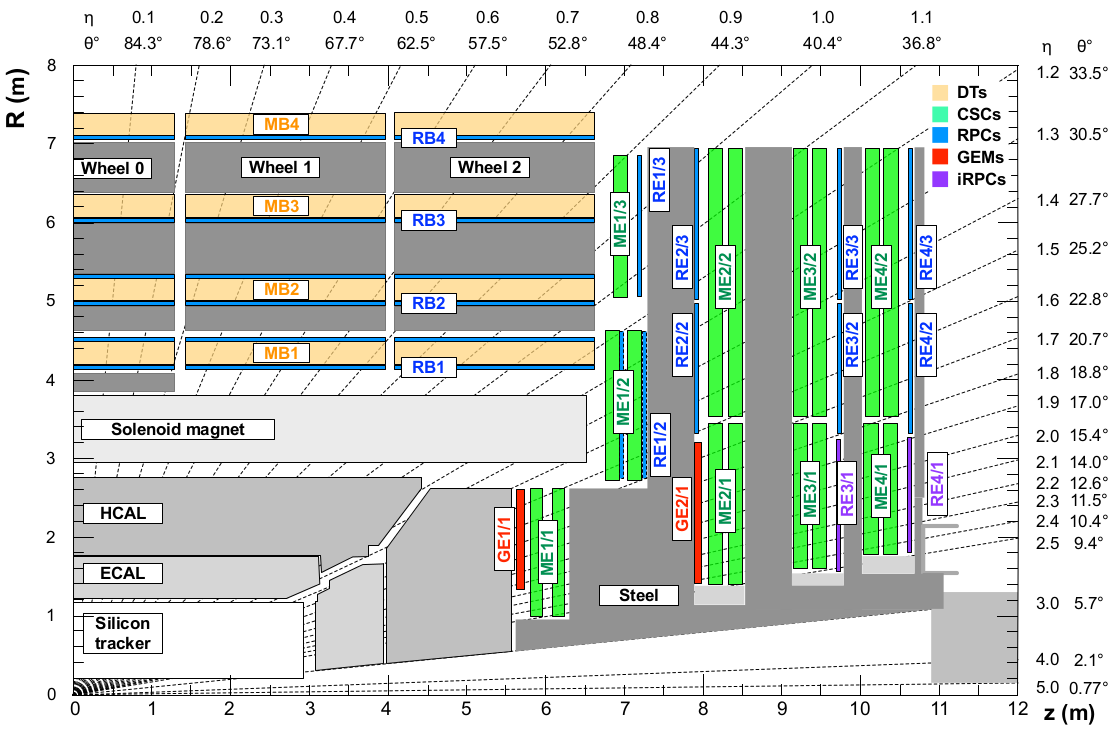
\includegraphics[width=.9\textwidth]{figures/cmsmuon.png}
  \caption{Section of CMS detector, in the plane $(r,z)$, parallel to the beamline, that emphasizes the location of the muon detectors, in particular: Drift Tubes (DT, in yellow); Cathode Strip Chambers (CSC, in green); Resistive Plate Chambers (RPC, in blue).}
  \label{fig:CMS_muon}
\end{figure}


\subsubsection{The Drift Tubes}
Drift Tube detectors cover a region of $|\eta|<1.2$ and are arranged in four stations, segmented along the beam line in five wheels. The basic element of the detector is the cell, that has a size of $42 \times 13 \text{ mm}^2$. Each cell is filled with a gas mixture (85\% argon, 15\% $\text{CO}_2$), in which the process of ionization takes places; the ionization electrons drift from the 50 $\mu$m thick steel anodic wire, located in the center of the cell, towards the aluminium cathodic strips, located at its edge. Additional electrodes on the surface of the cells allows to shape the electric field, in order to make the drift speed of the electrons uniform: the muon position is then extrapolated from the measurement of the drift time. Every station is composed by three cells superlayers. In the inner and the outer superlayers, the cells are oriented such in a way that the anodic wire is located along the $z$ axis, to measure the $\varphi$ coordinate. In the intermediate superlayer, wires are parallel to the radial coordinate, hence they can measure the $z$ position. The spatial resolution of the system is 100 $\mu$m in the $(r, \varphi)$ plane, 1 mrad in the $\varphi$ coordinate, and 150 $\mu$m in the longitudinal $z$ coordinate.

\subsubsection{The Cathode Strip Chambers}
Cathode Strip Chambers cover a region of $0.9<|\eta|<2.4$, overlapping with the DTs in the pseudorapidity range $0.9 < |\eta| < 1.2$. The anodic wires inside each CSC are installed in six planes, with the aim of measuring the radial coordinate; the wire planes are perpendicularly crossed by cathodic strips, disposed along the radial direction to measure the $\varphi$ coordinate. Ionization electrons produced by muons passing through the gas mixture in the chambers migrate from the anodes, inducing a charge distribution on the cathodes, from which the azimuthal coordinate can be reconstructed. The spatial resolution %in the $r$ coordinate is 200 $\mu$m, and it 
is 75 -- 150 $\mu$m in the $(r, \varphi)$ plane. CSCs are arranged in four disks and in three concentric rings.

\subsubsection{The Resistive Plate Chambers}
Resistive Plate Chambers are located both in the barrel (disposed in six layers) and in the endcap region (three layers), up to a pseudorapidity of $|\eta|<1.6$. These gas detectors are charged at very high voltages, in order to work in the avalanche ionization mode. The plastic resitive plates are equipped with readout strips. The spatial resolution of the detector is low (1-2 cm), but the fast timing response (2-3 ns) and good time resolution (1 ns) allow to employ RPCs as an additional triggering system and to profit of a precise measurement of the bunch-crossing time.

%\subsection{Other CMS sub-detectors}
%Tracciatori e camere per i muoni coprono una regione di $|\eta|<2.5$, gli apparati calorimetrici arrivano fino ad $|\eta|<5.2$. Ci sono altri due rivelatori che permettono misure nella regione $5 \leq |\eta| \leq 11$, TOTEM e CASTOR. TOTEM sfrutta dei rivelatori a gas per le misure di scattering elastico protone protone in funzione del loro momento. CASTOR \`e un calorimetro elettromagnetico ed adronico che raccoglie luce Cherenkov, serve per misure di QCD in collisioni p-p, p-ione, ione-ione.

\subsection{The trigger system and data acquisition}
The CMS trigger system~\cite{TRIG-TDR} has been designed considering the high instantaneous luminosity, such that it can provide a fast response and it allows to reduce the nominal event rate of 40 MHz in proton proton collision. The complexity of the CMS detector and the very high number of readout channels result into a huge amount of data per event, approaching the order of few MB per bunch crossing, hence 40 TB per second. The processes of handling and recording data are currently limited by the employed technology to a frequency of $\sim$100 Hz. Applying online selections to skim the events that are going to be written on tape, without rejecting interesting signals of hard processes and rare phenomena, is therefore a crucial and challenging point for every data analysis. Events are filtered by trigger selections at different levels: the Level-1 (L1) trigger is an hardware device, that allows to reduce the event rate from 40 MHz to the order of 100 kHz; the High Level Trigger (HLT) is a set of software algorithms that skims the event rate down to few hundred Hz. Once the trigger decisions are taken, the final events are handled by the Data Acquisition System (DAQ), that collects the informations coming from the sub-detectors and sends them to the storage unities.

\subsubsection{The Level-1 trigger}
The L1 trigger is an hardware device composed by customized electronics, and it accesses the informations coming from the calorimeters and the muon system, while the tracker is not considered given the excessively large bandwidth needed by its readout channels. The L1 trigger performs a first raw local reconstruction of each object, called ``trigger primitive''. The L1 trigger is composed by three subsystems: the calorimeter trigger, the muon trigger (divided in three independent sub-subsystems for each muon sub-detector, DTs, RPCs and CSCs), and the global trigger, that combines the informations of the former subsystems. The best quality trigger primitives reconstructed by the calorimeters and muon detectors (namely, roughly reconstructed electrons, photons, muons, jets, jets coming from the hadronic decays of tau leptons, and missing transverse energy) are handled by the global trigger, which takes the decision of discarding or keeping the event every 3.2 $\mu$s. The simplest trigger selections require the presence of a single object, whose energy or transverse momentum is higher than a certain threshold; more complicated triggers involve multiple objects or geometrical selections, that can be performed in parallel up to 128 simultaneous requirements.

\subsubsection{The High Level Trigger}
The HLT skims the L1 output rate down to few hundreds Hz by applying a set of algorithms, implemented in the same software used for the offline analyses, consisting in an event reconstruction performed by exploiting the whole informations coming from all sub-detectors. The computing time is still a crucial factor, hence selections applied to HLT physics objects are generally less accurate than those of the offline analyses; furthermore, HLT can discard the event even before its full reconstruction (\textit{i.e.} by looking only at certain region of the detectors). Events filtered by the HLT decisions are assigned to precise trigger paths and recorded in different categories of datasets.

\subsubsection{Data acquisition, computing and storage}
The DAQ system deals with the storage, transfer and handling of the data collected by CMS; it also supports and stores the data simulations and calibrations of the sub-detectors. The CMS computational resources are located in worldwide distributed data nodes, called Tiers. The CMS software (CMSSW) is based on an object oriented architecture (mainly C++). The basic unity of every data, both real and simulated ones, is the Event, that could contain very rough informations (RAW data format) or higher level refined objects (AOD, Analysis Object Data) where all the calibrations and corrections needed to properly deal with the final physics objects are already in place. Data are handled by C++ or python modules, and the outputs are written in ROOT~\cite{Brun:1997pa} files.

\subsection{Particle Flow event reconstruction}
The particle flow (PF) algorithm~\cite{Sirunyan:2270046} aims at identifying and reconstructing each particle produced by the proton-proton collisions, combining the informations coming from all the CMS sub-detectors. It is particularly suitable to improve the reconstruction of jets, missing transverse momentum (used to identify neutrinos) and hadronically decaying tau leptons.\\
The association of the informations is performed at different stages. The reconstruction of the charged particles in the silicon detector is executed with an iterative algorithm, and the reconstructed object is called a tracker track. Then, a clustering algorithm is performed to collect and combine the energy deposits in the calorimeters, in such a way to distinguish neutral from charged particles, reconstruct their directions, and improve the energy measurement of the very energetic charged particles, whose tracks are less bended by the magnet and hence less precisely determined. The last informations are provided by the hits collected in the muon system. The three sets of reconstructions are then combined with a link algorithm, that aims at associating tracker tracks to calorimeter clusters and muon hits with geometrical criteria. A track in the silicon detector is linked to a calorimeter cluster if the extrapolated position lies in the cluster itself. Similarly, clusters in different calorimeters are linked when the position calculated in the more granular calorimeter (\textit{i.e.} ECAL) lies in the envelope of the clusters in the less granular calorimeter (\textit{i.e.} HCAL). The decision of linking a tracker track to a muon track is based on the $\chi^2$ of a global fit between the two tracks.\\
The particle flow algorithm then interprets the collected and linked informations as particles. Muons are identified by the combination of a track in the silicon detectors and a track in the muon chambers. Photons are determined directly by ECAL clusters. Electrons energies and positions are measured by ECAL clusters, linked to a corresponding tracker track, and considering all the energy clusters produced by the bremsstrahlung photons radiated while interacting with the detector material. The hadrons are identified by the tracks (if charged) linked to the corresponding ECAL and HCAL clusters. The hadron energy resolution, 10\% at 100 GeV combining ECAL and HCAL, is such that neutral hadrons can be distinguished as an energy calorimetric excess when overlapped by a charged hadron occupying the same calorimetric towers. Finally, the missing transverse momentum is defined as the negative sum of the transverse momenta of all the particles identified by the PF algorithm.\\

\subsection{Physics objects}
\label{ssec:physicsobjects}

\subsubsection{Track reconstruction}
The reconstruction of the trajectories of the charged particles passing through the CMS detector is performed by multiple iterations of the Combined Track Finder algorithm, that is based on a Kalman filter approach~\cite{Fruhwirth:1987fm}; given the high multiplicity of particles produced at each bunch crossing and the multiple scatterings in the detector materials, tracking represents a challenging task. The CTF algorithm builds a track starting from the so-called seeds, namely triplets of hits collected in the pixel detector inner layers, or couples of hits if the track originates from the interaction point. The initial guess of the track given by the seeds is then extrapolated to the outer layers: if other hits are found to be compatible with the trajectory hypotesis ($\chi^2$-based hypotesis test), they are added to the track. Once the outer layers are reached, another reconstruction is performed backward, in order to clean the track from spurious hits and enhance the tracking efficiency. The final collected hits are re-fitted with Kalman filter and more precise algorithms, in order to improve the quality of the measurement. If two tracks share more than a half of their hits, the worst quality track is rejected. The track reconstruction efficiency for particles with $p_T >0.9$ GeV is 94\% in the barrel and 85\% in the endcap region~\cite{Chatrchyan:2014fea}.\\


\subsubsection{Vertices reconstruction}
The reconstruction of the vertices at each bunch crossing is performed in steps. Primary vertices are originating from the proton proton collisions, whilst secondary vertices are due to long-lived particles (heavy quarks and $\tau$ leptons). The starting point of the procedure is clustering the reconstructed tracks originating from the primary vertex; the decision is taken by the deterministic annealing algorithm~\cite{bib:detanneal}, taking as input the longitudinal impact parameter. The algorithm allows to distinguish vertices separated down to 1 mm. The second step is run by the adaptive vertex fitter~\cite{Fruhwirth:2007hz}, that measures the position of the vertex for the chosen set of tracks. The algorithm is based on an iterative re-weighted Kalman filter, that down-weights the wrongly associated tracks not compatible with the considered vertex. The primary vertex is selected as the vertex where the sum of the $p_T^2$ of the associated tracks is the largest. The spatial resolution on the vertex position is 10-40 $\mu$m in the $(r, \varphi)$ plane, and 15-50 $\mu$m in the longitudinal coordinate.

\subsubsection{Electrons and photons reconstruction}
Electrons are reconstructed~\cite{Chatrchyan:2013dga} combining a track with the energy deposits clustered in the ECAL, due to the showering of the electron through the detector and the emission of bremsstrahlung photons. The combination can proceed both from the silicon detector in the outgoing direction and in the opposite way: the tracker seeding as starting point is suitable for low energy electrons, whose trajectories are less bended and hence more accurately measured by the tracker system; the grouping of ECAL clusters (called superclusters) followed by a consecutive track extrapolation, performed by taking into account the electron interaction with the detector material, is more efficient in case of high energetic electrons, due to the higher resolution of the ECAL scintillating crystals. A Gaussian-sum filter algorithm (GSF)~\cite{Adam:2005bya} allows to properly take into account the effects of the bremsstrahlung radiation, that is distributed not as a single Gaussian (standard Kalman filters) but rather as a sum of Gaussian functions.\\
The identification of an electron relies on three groups of variables: observables built by combining measurements performed in the silicon detectors and in the calorimeter; purely calorimetric observables; purely tracking informations. Different selections are used for electron candidates found in the barrel or in the endcaps, and they can vary from loose criteria (high detection efficiency but less purity, namely more contamination from object mis-identified as electrons) to tight criteria. Data and Monte Carlo simulations reproducing $Z$, $\Upsilon$ and $J/\Psi$ decays in $e^+ e^-$ are used to study the optimal working points, each one targetting at a different purity.\\
The electron energy is determined correcting the raw energy measurement of the ECAL superclusters by taking into account the effects of the losses due to radiation or gaps between the calorimeter modules, and the pile-up contribution. The electron momentum resolution has been measured in $Z \rightarrow e^+ e^-$ decays in Run 1 LHC data, and it varies from 1.7\% to 4.5\% depending on the pseudorapidity range~\cite{Khachatryan:2015hwa}. %With respect to traditional supercluster corrections, this technique improves the electron resolution by about 10\%.
The electron isolation variable is defined as the $p_T$ sum of the charged and neutral particles lying in a cone of $\Delta R = 0.3$ around the electron trajectory, divided by the transverse momentum of the electron itself:
\begin{equation}
I_{\Delta R = 0.3}^e = \frac{\sum_{\text{char. hadrons}} p_T + max\left[ 0, \sum_{\text{neut. hadrons}} p_T + \sum_{\text{photons}} p_T - 0.5 \sum_{\text{pile-up char. hadrons}} p_T\right]}{p_T^e};
\label{eq:electron_iso}
\end{equation}
the contribution of the pile-up charged particles is removed. The isolation variable is used to distinguish electrons coming from the leptonic decays of electroweak bosons (low $I_{\Delta R = 0.3}^e$) from electrons coming from the decays of heavy fermions, when they are more likely produced in association with light flavour jets and hence topologically close to calorimetric deposits due to hadrons (high $I_{\Delta R = 0.3}^e$).

\vspace*{1\baselineskip}

\noindent Photons are reconstructed with the ECAL clusters only. Given their importance in the discovery of the Higgs boson, dedicated studies have been performed both in data and in Monte Carlo simulations reproducing the $H \rightarrow \gamma \gamma$ process. Particular care has been taken in the treatment of the photon conversions into electron-positron pairs while interacting with the tracker detector. Dedicated selections allow to define different photon identification working points. Similarly to the case of the electrons, the photon isolation variable can be defined. The photon energy resolution varies from 1\% to 3\%, depending on the $\eta$ range~\cite{Khachatryan:2015iwa}.

\subsubsection{Muon reconstruction}
A muon candidate can be built exploiting the hits collected in the silicon tracker (track) and in the muon system (standalone muon)~\cite{Chatrchyan:2012xi}. Each muon sub-detector (DTs, RPCs and CSCs) performs a local reconstruction of the particle candidate; the informations from the three muon chambers are combined with a Kalman filter approach.\\
Three different strategies are adopted to define a muon candidate in the CMS detector. A standalone muon is reconstructed by using only the local reconstruction in the muon chambers. A tracker muon is built starting from a track in the silicon detector, that is extrapolated up to the muon chambers, taking into account the multiple scattering and the energy loss through the material. The tracker muon is defined if at least one segment, \textit{i.e.} a short track built with CSCs or DTs hits, is matched to the starting track. This technique is the most efficient for the reconstruction of low energetic muons. A global muon is built starting from a standalone muon, and then its trajectory is extrapolated towards the inner layer of the silicon detector and eventually matched to a track; this approach is suitable for high energetic muons ($p_T>200$ GeV).\\
Different algorithms are used to assign a momentum to the muon candidate, in order to mitigate the effects of bremsstrahlung, that becomes significant when the muon approaches energies of the order of 1 TeV. The radiated photons generate spurious hits in the chambers and larger occupancy, significantly deteriorating the momentum measurement.\\
Starting from 2016 LHC Run, the muon reconstruction takes into account the Alignment Position Errors, namely the uncertainties due to the position of the muon chambers with respect to the silicon detectors. The final resolution on the muon momentum measurement depends on the $p_T$ and $\eta$ of the candidate, and ranges from 1\% for very low momenta, up to $\sim$7\% ($|\eta|<0.9$) -- 10\% ($1.2 < |\eta| < 2.4$)~\cite{CMS-DP-2016-067}.\\
The muon isolation $I_{\Delta R = 0.4}^{\mu}$ is defined similarly to the electron isolation, but by taking into account a larger cone $\Delta R = 0.4$ around the muon direction.

\subsubsection{Jet reconstruction}
The nature of the strong interaction is such that coloured partons, namely quarks and gluons, are forced to aggregate to form a color-neutral hadron, in the process called hadronization. Therefore, partons cannot be observed as free particles in a detector, but rather as collimated jets of hadronic particles.\\
Jets are reconstructed starting by the PF candidates in the event. The charged hadron subtraction algorithm (CHS) removes candidates not associated to the primary vertex in order to suppress pile-up contributions~\cite{CMS-PAS-JME-14-001}. The remaining particles are used as input to jet clustering algorithms
to reconstruct particle flow jets. The jets are clustered using the {\sc FastJet} package~\cite{Cacciari:2011ma} with the anti-\kt jet sequential clustering algorithm~\cite{Cacciari:2008gp}. A sequential clustering algorithm is designed to be infrared and collinear safe, namely, if the final state particles undergo a soft emission or a collinear gluon splitting, the number and shapes of the jets should not change. The starting point of a sequential clustering algorithm is the definition of the distances bewtween two particles $i$ and $j$, and the distance of a given particle $i$ from the beam-spot $B$:
\begin{equation}
\begin{split}
& d_{ij} = \min \left( p_{T,i}^{2a} p_{T,j}^{2a} \right) \frac{R_{ij}^2}{R_0^2},\\
& d_{iB} = p_{T,i}^{2a}\\
\end{split}
\label{eq:dist_akt}
\end{equation}
where $p_{T(i,j)}$ are the transverse momenta of the particles, $R_{ij}^2 = \left( \rap_i - \rap_j \right)^2 + \left( \varphi_i - \varphi_j\right)^2$ is the angular distance between the particles, $a$ is an exponent depending on the clustering algorithm chosen, and $R_0$ is the clustering parameter. The algorithm then operates as follows:
\begin{itemize}
\item it computes all the possible combinations of distances $d_{ij}$ and $d_{iB}$ and it finds the minimum;
\item if the minimum is $d_{ij}$, the four-momenta of the particles $i$ and $j$ are summed up in one candidate $ij$; $i$ and $j$ are removed from the list of available particles, the distances are updated, and the algorithm proceeds to re-calculate all the possible remaining $d_{ij}$;
\item the clustering stops when the smallest quantity is $d_{iB}$: $i$ particle is defined as one jet, and it is removed from the list of particles;
\item this process is repeated until all the particles are assigned to a jet, that must be separated from another jet at least by a distance $R_{ij} > R_0$.
\end{itemize}
If the anti-\kt algorithm is applied, the exponent $a = -1$. This means that it tends to cluster high \pt particles first, given that the hard term dominates $d_{ij}$ in equation~\ref{eq:dist_akt}. Since the soft particles have lower impacts, the shape of the jet is not sensitive to the soft radiation and rather stable against the softer pile-up contributions.\\
In this analysis, clustering parameters of $R_0 = 0.8$ and $R_0 = 0.4$ will be used to define the ``fat''-jets or AK8 jets, and the ``standard''-jets or AK4 jets. In order to avoid double-counting of PF candidates, AK4 jets are considered only if the angular separation from the leading AK8 jet is larger than $R_0>0.8$.\\
Since the detector response to different particles is non-linear, particular care should be taken in the assignement of the measured momentum of the clustered jet to the corresponding true value of the original parton~\cite{bib:1748-0221-6-11-P11002}. A set of jet energy corrections (JECs) are applied sequentially and with a fixed order. Each correction constists in a rescaling of the jet four-momentum, and it takes into account different effects that are factorized.
\begin{itemize}
\item The L1 JECs remove the effect of the pile-up; they consist into an offset correction of the jet \pt. They are determined from Monte Carlo (MC) simulations of di-jet events produced by strong interaction with and without pile-up events on top, and parametrized as a function of kinematical variables (jet area, pseudorapidity and \pt) and of the average \pt density per unit area, $\rho$. Residual differences between data and the detector simulation are evaluated in data collected with a random trigger, called zero bias, applying the only requirement of the beam crossing happening. Pile-up offset corrections are displayed in fig.~\ref{fig:plot_JEC} (top left), as a function of the jet pseudorapidity.
\item The simulated response of the detector is not uniform over jet \pt and $\eta$. This effect is mitigated by the L2L3 MC-truth corrections. They are calculated in MC simulations of di-jet events, by taking into account the discrepancy between the reconstructed \pt of the jet and the true \pt at particle generator level (\textit{i.e.}, before simulating the interaction of the parton showers with the detector), as a function of jet \pt and $\eta$. L2L3 scale factors describing the simulated jet response are reported in fig.~\ref{fig:plot_JEC} (top right), as a function of the jet pseudorapidity.
\item The small data-MC discrepancies ($\sim$1\%) left after applying the previous set of JECs are corrected by the L2 and L3 residual corrections. The L2Residuals are calculated in di-jet events, as a function of \pt. The L3Residuals are calculated in $Z \rightarrow (\mu \mu, ee)$ + jet events, photon + jet events and multijet events, as a function of $\eta$ and \pt%, with the \pt-balancing method
~\cite{bib:1748-0221-6-11-P11002}. Data-MC scale factors for L2L3Residuals are displayed in fig.~\ref{fig:plot_JEC} (bottom), as a function of the jet $\eta$ and \pt.
\item An optional correction, not used in this analysis, is the L5 flavour-dependent correction, that is extracted from MC simulations.
\end{itemize}

\begin{figure}[!htb]
  \centering
    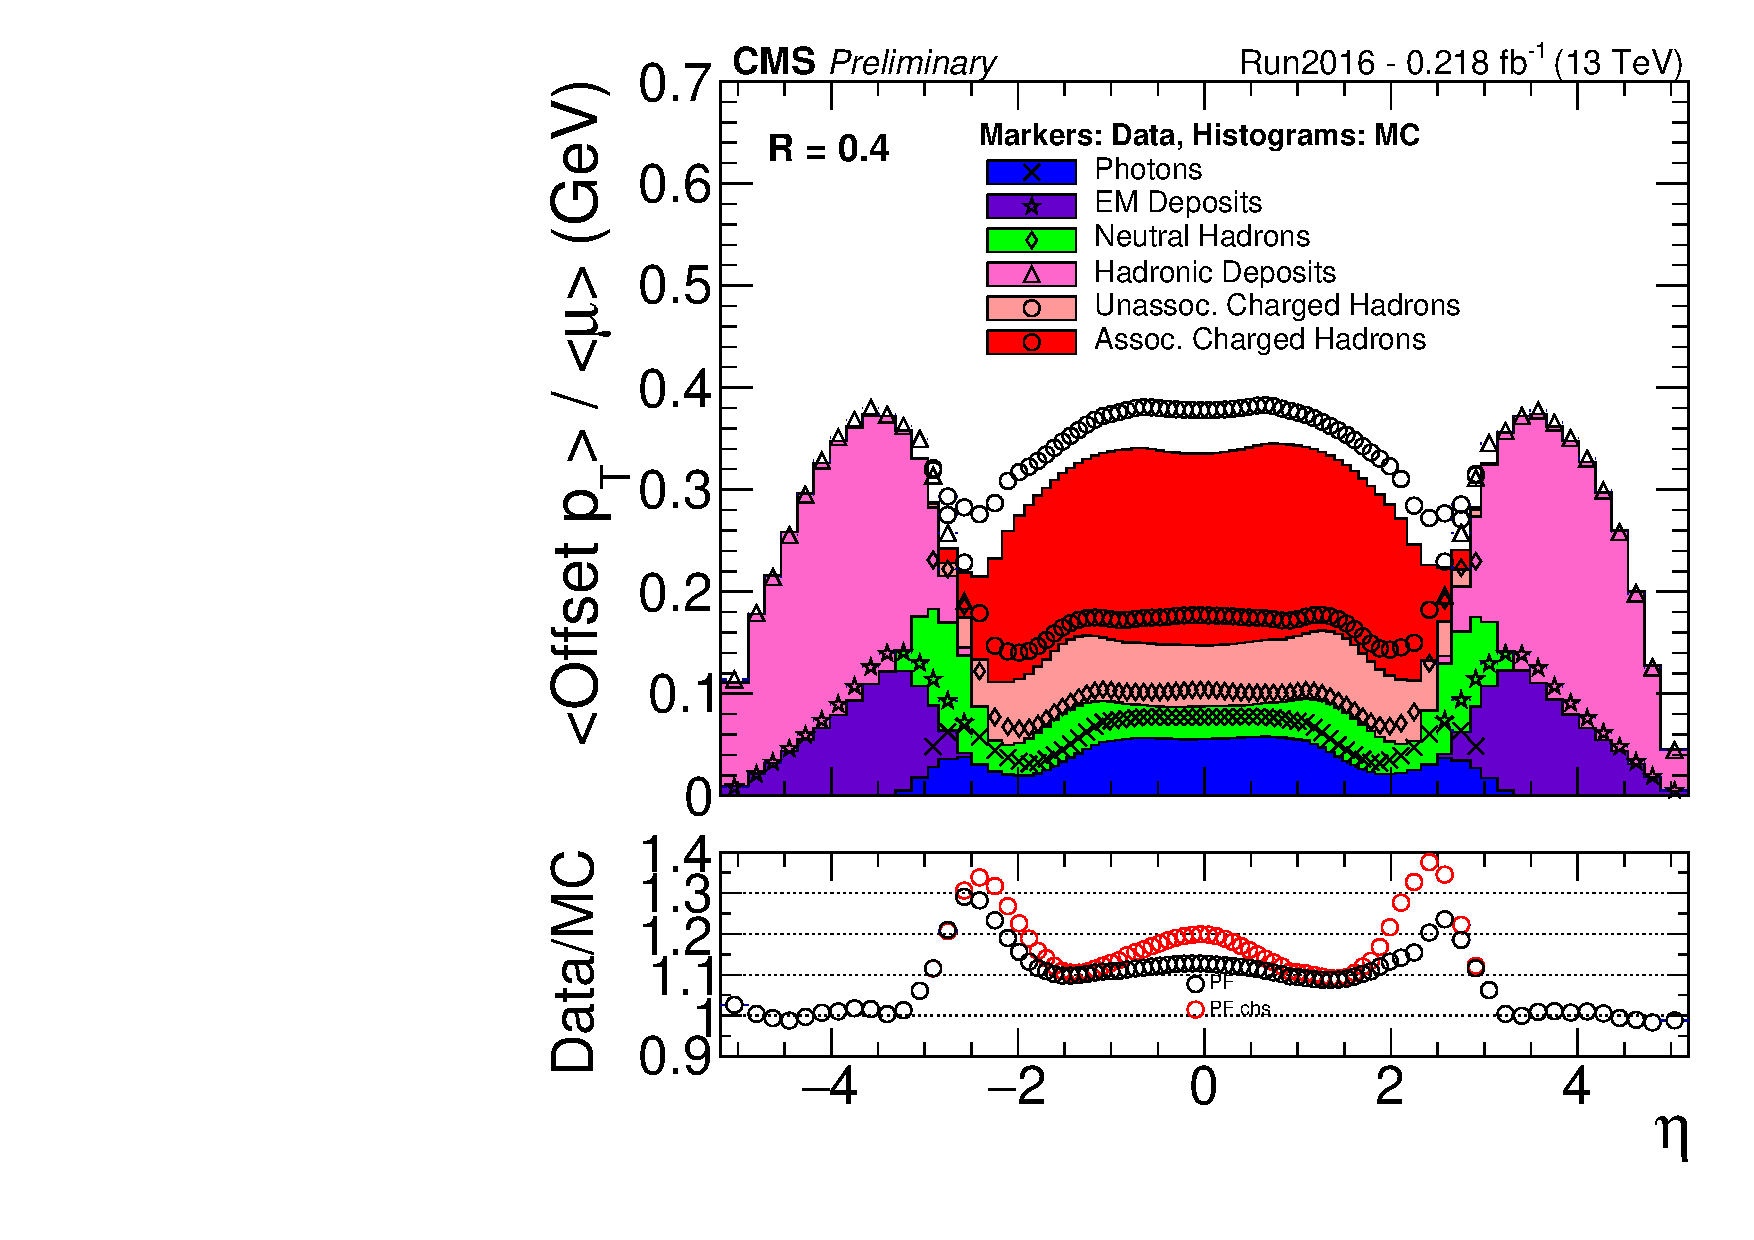
\includegraphics[width=.5\textwidth]{figures/JetPlots/stack2016.pdf}%
    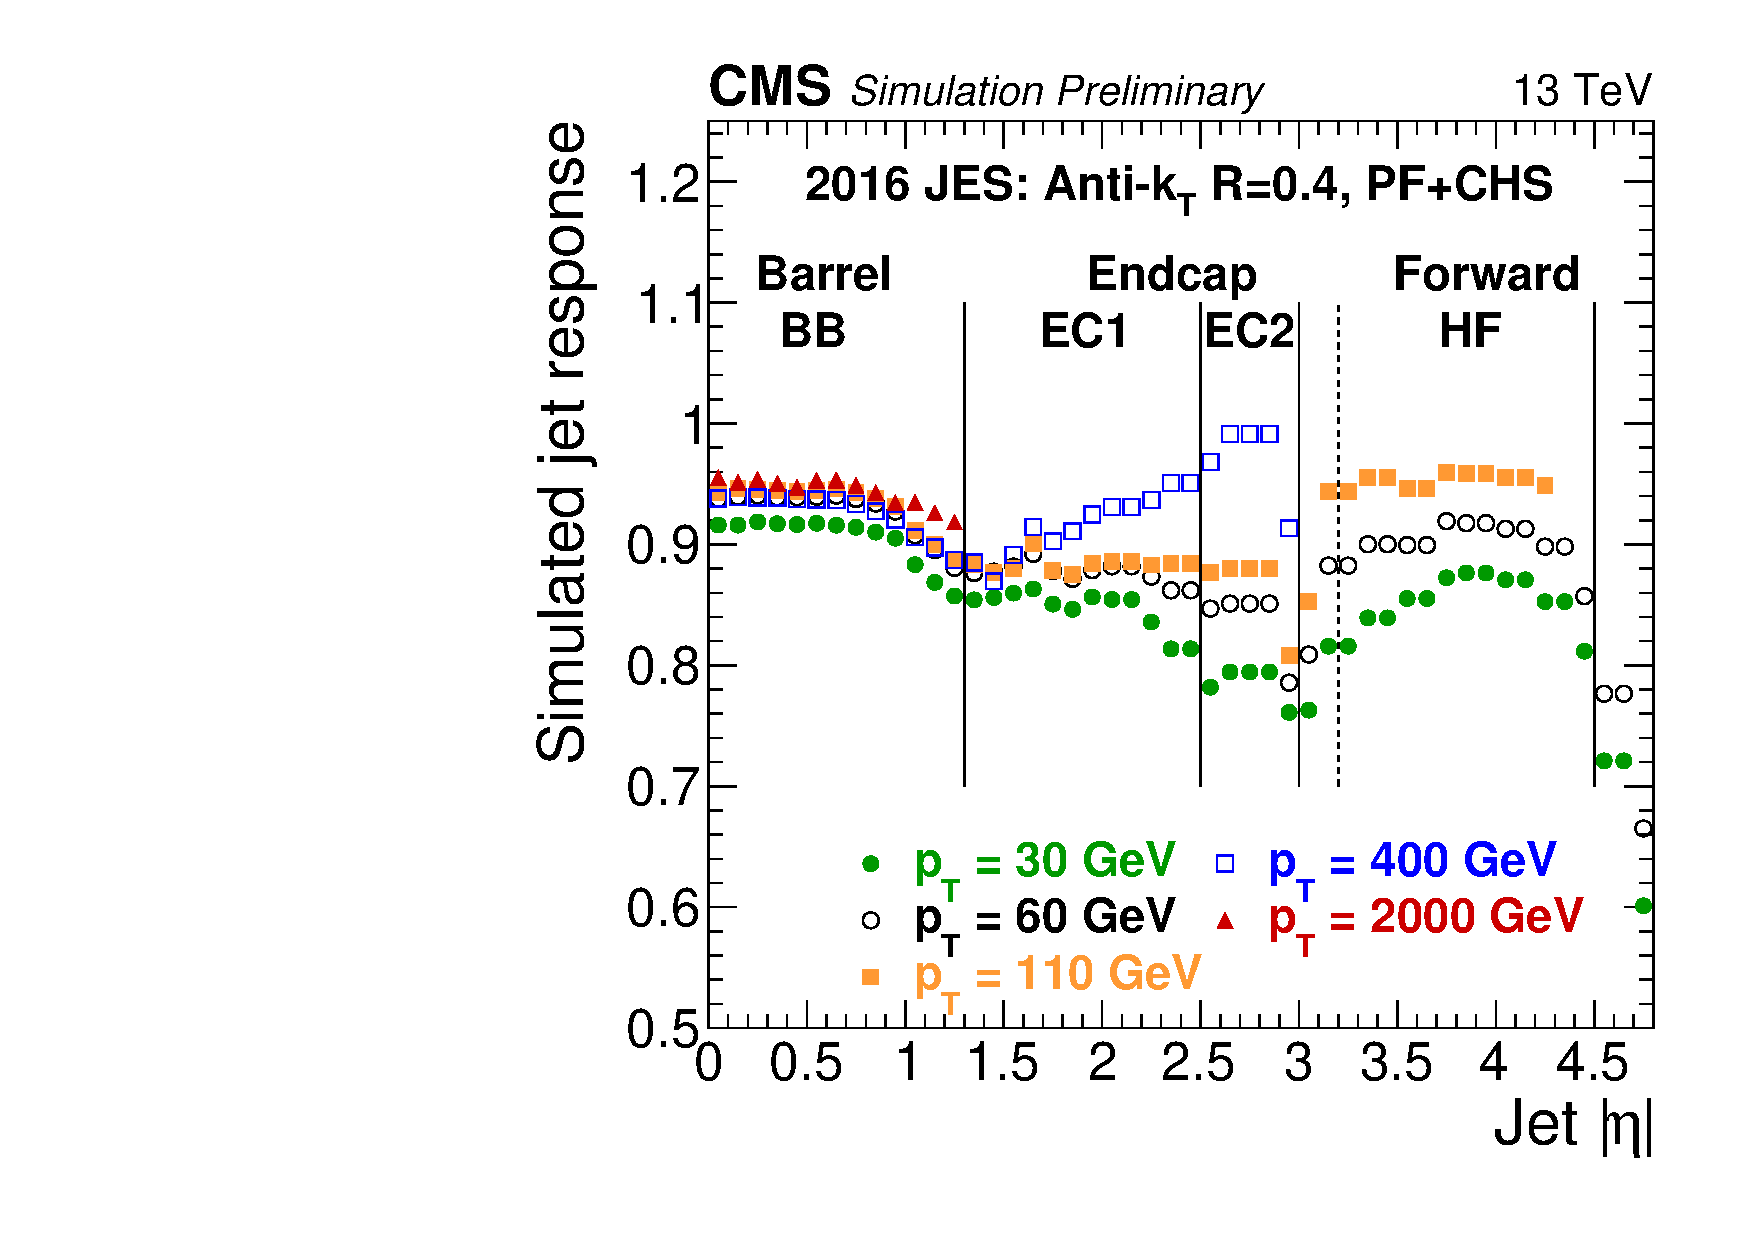
\includegraphics[width=.5\textwidth]{figures/JetPlots/CMSresponse_ak4pfchs_L1FastL2L3.pdf}
\\
    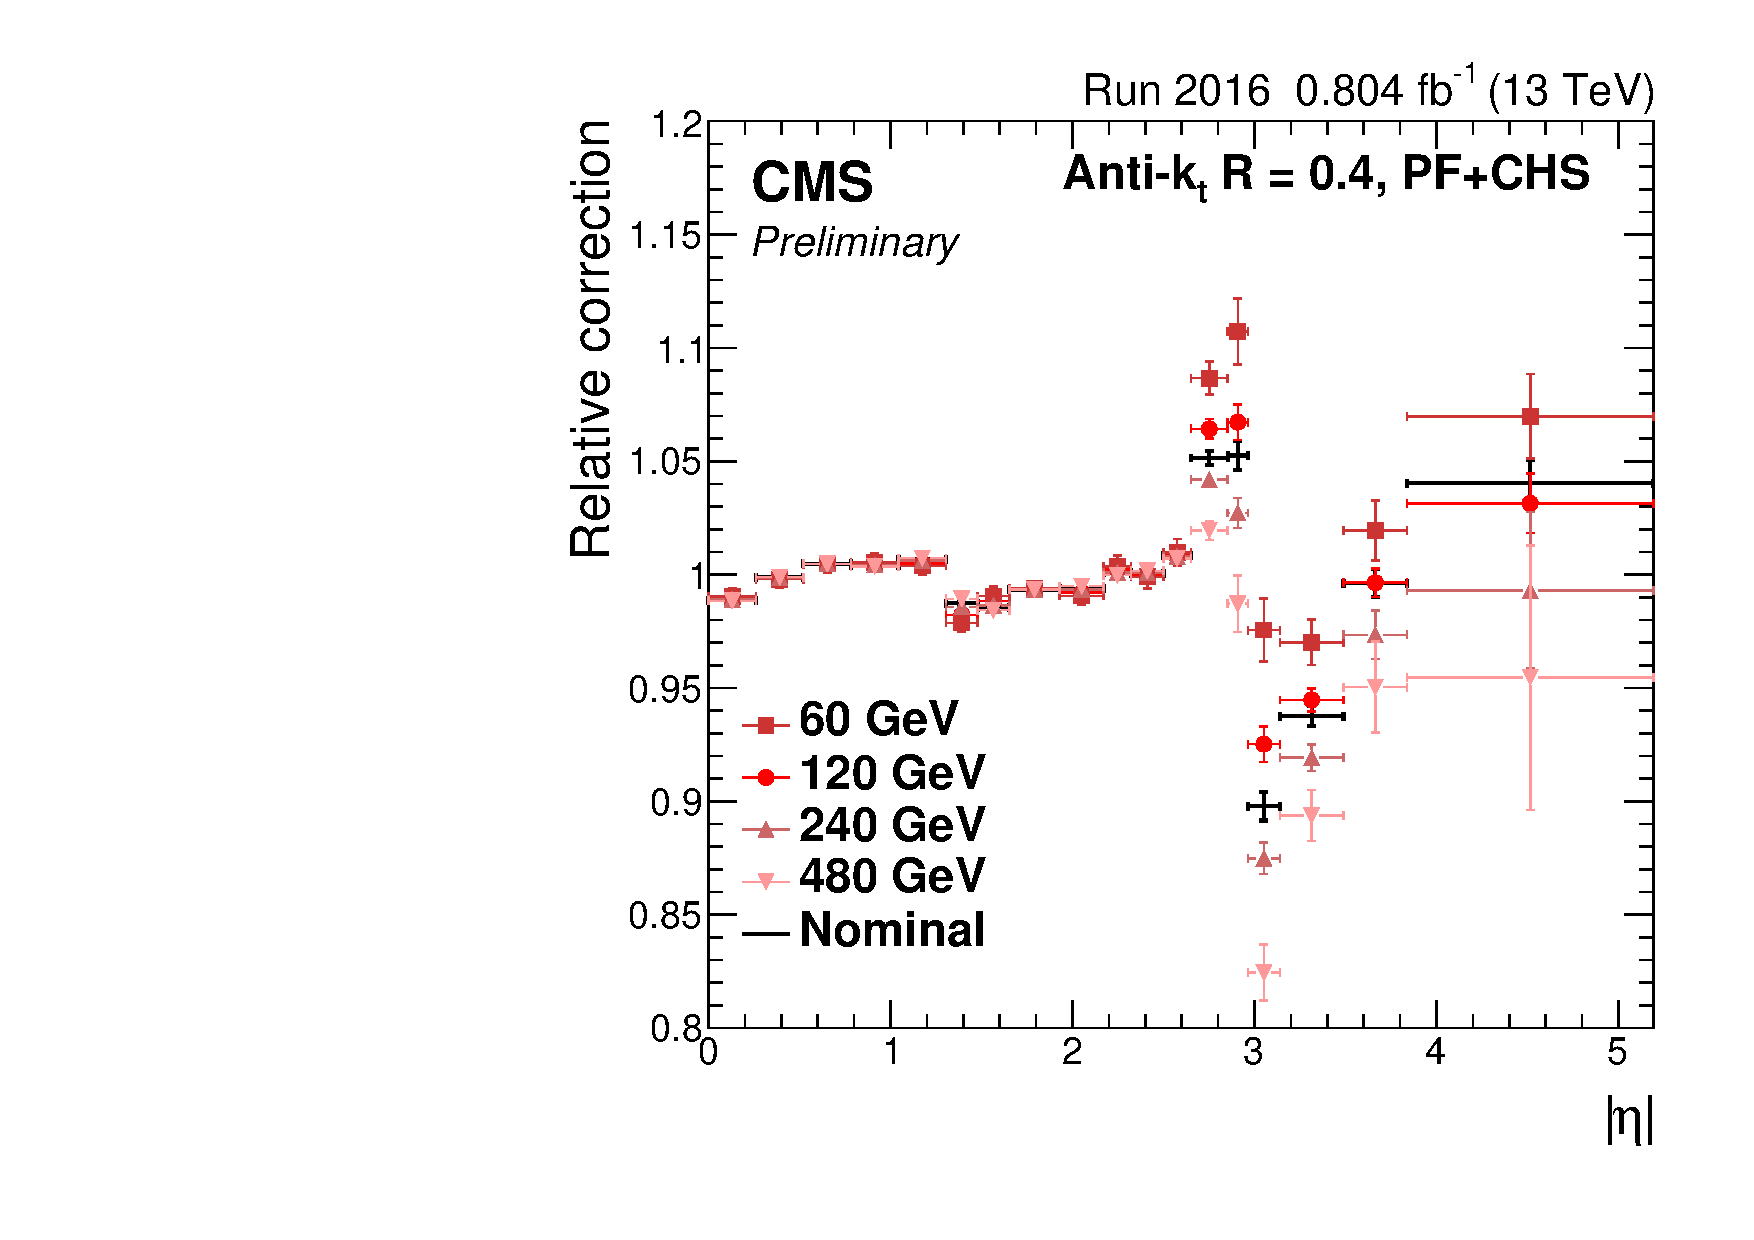
\includegraphics[width=.5\textwidth]{figures/JetPlots/L2Res_logpt_MPF_kFSRfit_AK4PFchs_pythia8_2016.pdf}%
    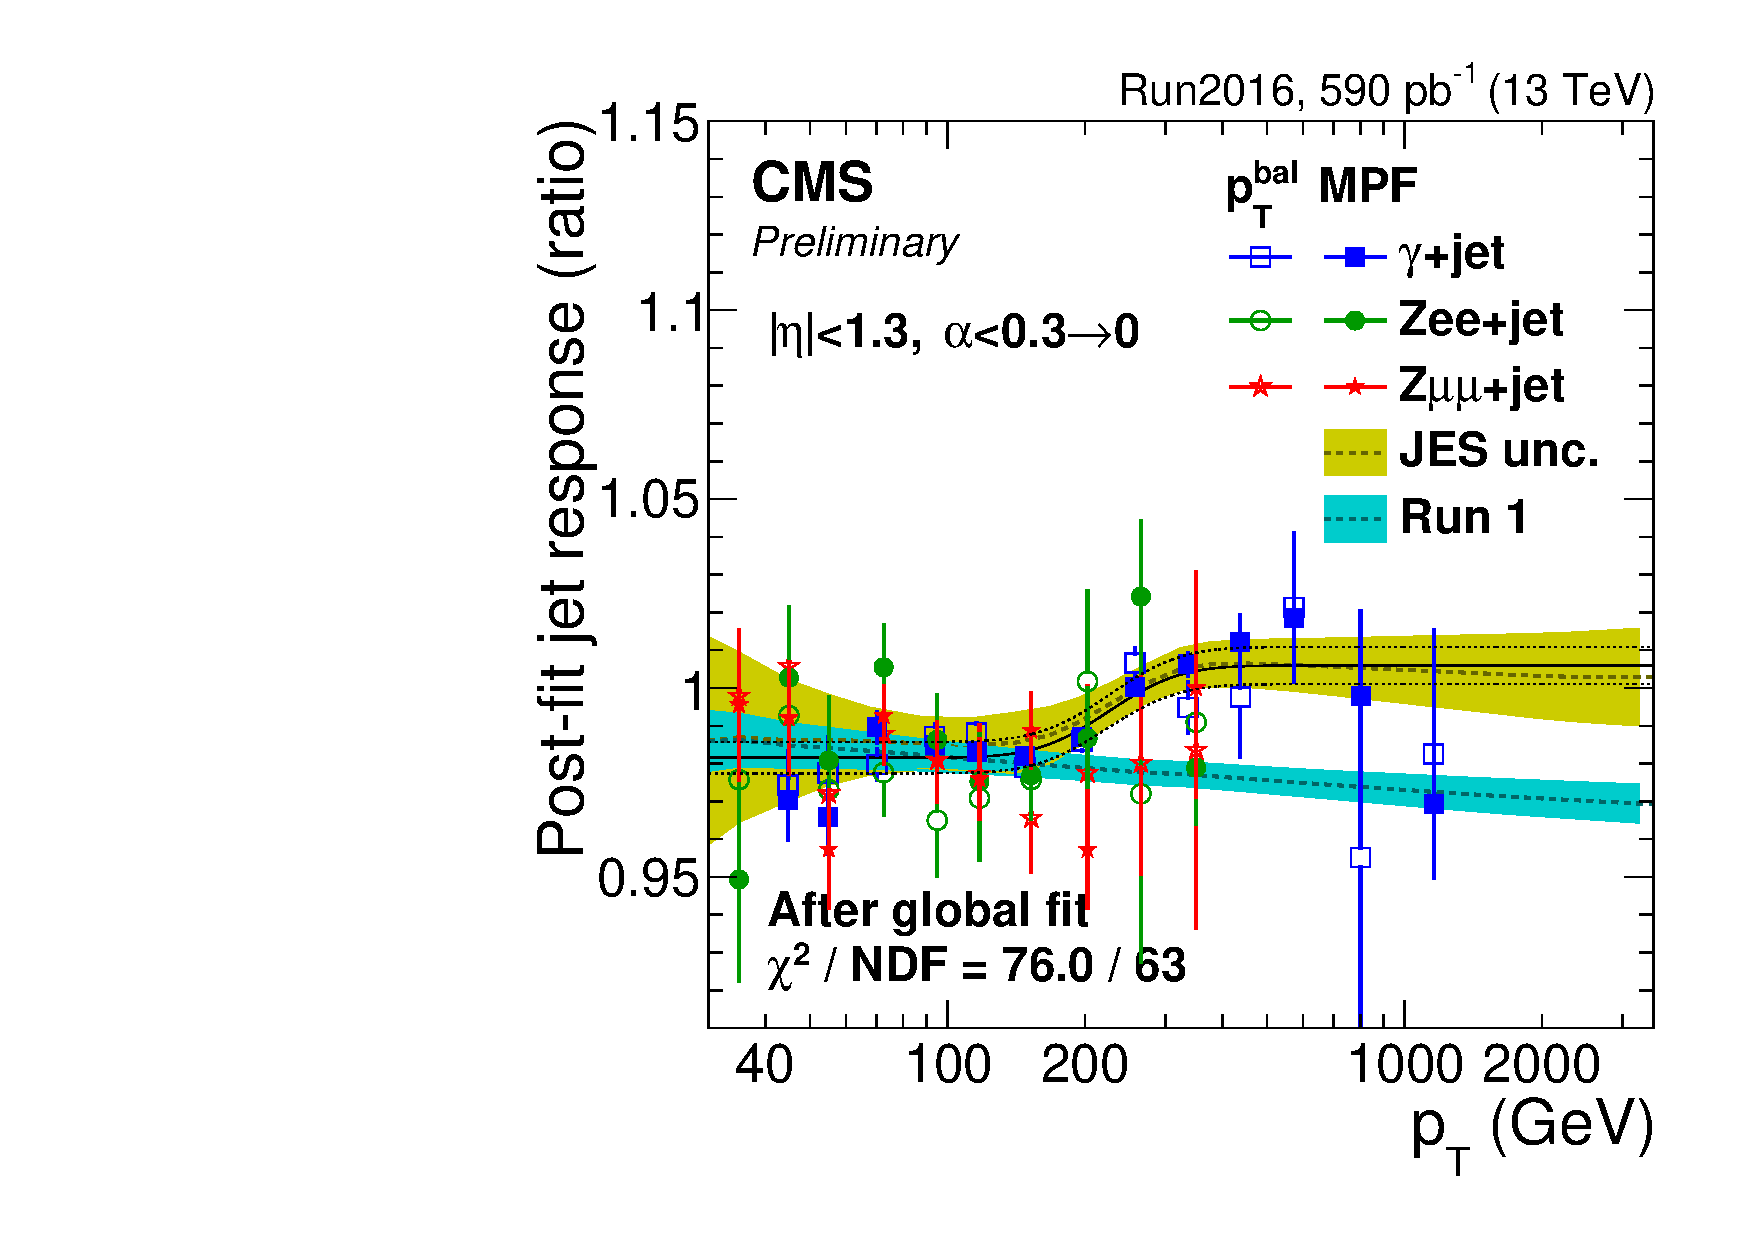
\includegraphics[width=.5\textwidth]{figures/JetPlots/globalFitL3res_shifted_2016.pdf}

  \caption{Top left: average \pt offset due to additional pile-up events, measured both in data and in MC simulations, as a function of the jet pseudorapidity. Top right: simulated jet response (L2L3 MC-truth corrections), as a function of the jet pseudorapidity. Bottom left: L2L3 residual data-MC corrections, evaluated on di-jet events, as a function of the jet $\eta$. Bottom right: L2L3 residual data-MC corrections, evaluated on di-jet and $Z/\gamma$ + jet events, as a function of the jet \pt.}
  \label{fig:plot_JEC}
\end{figure}

\begin{figure}[!htb]
  \centering
    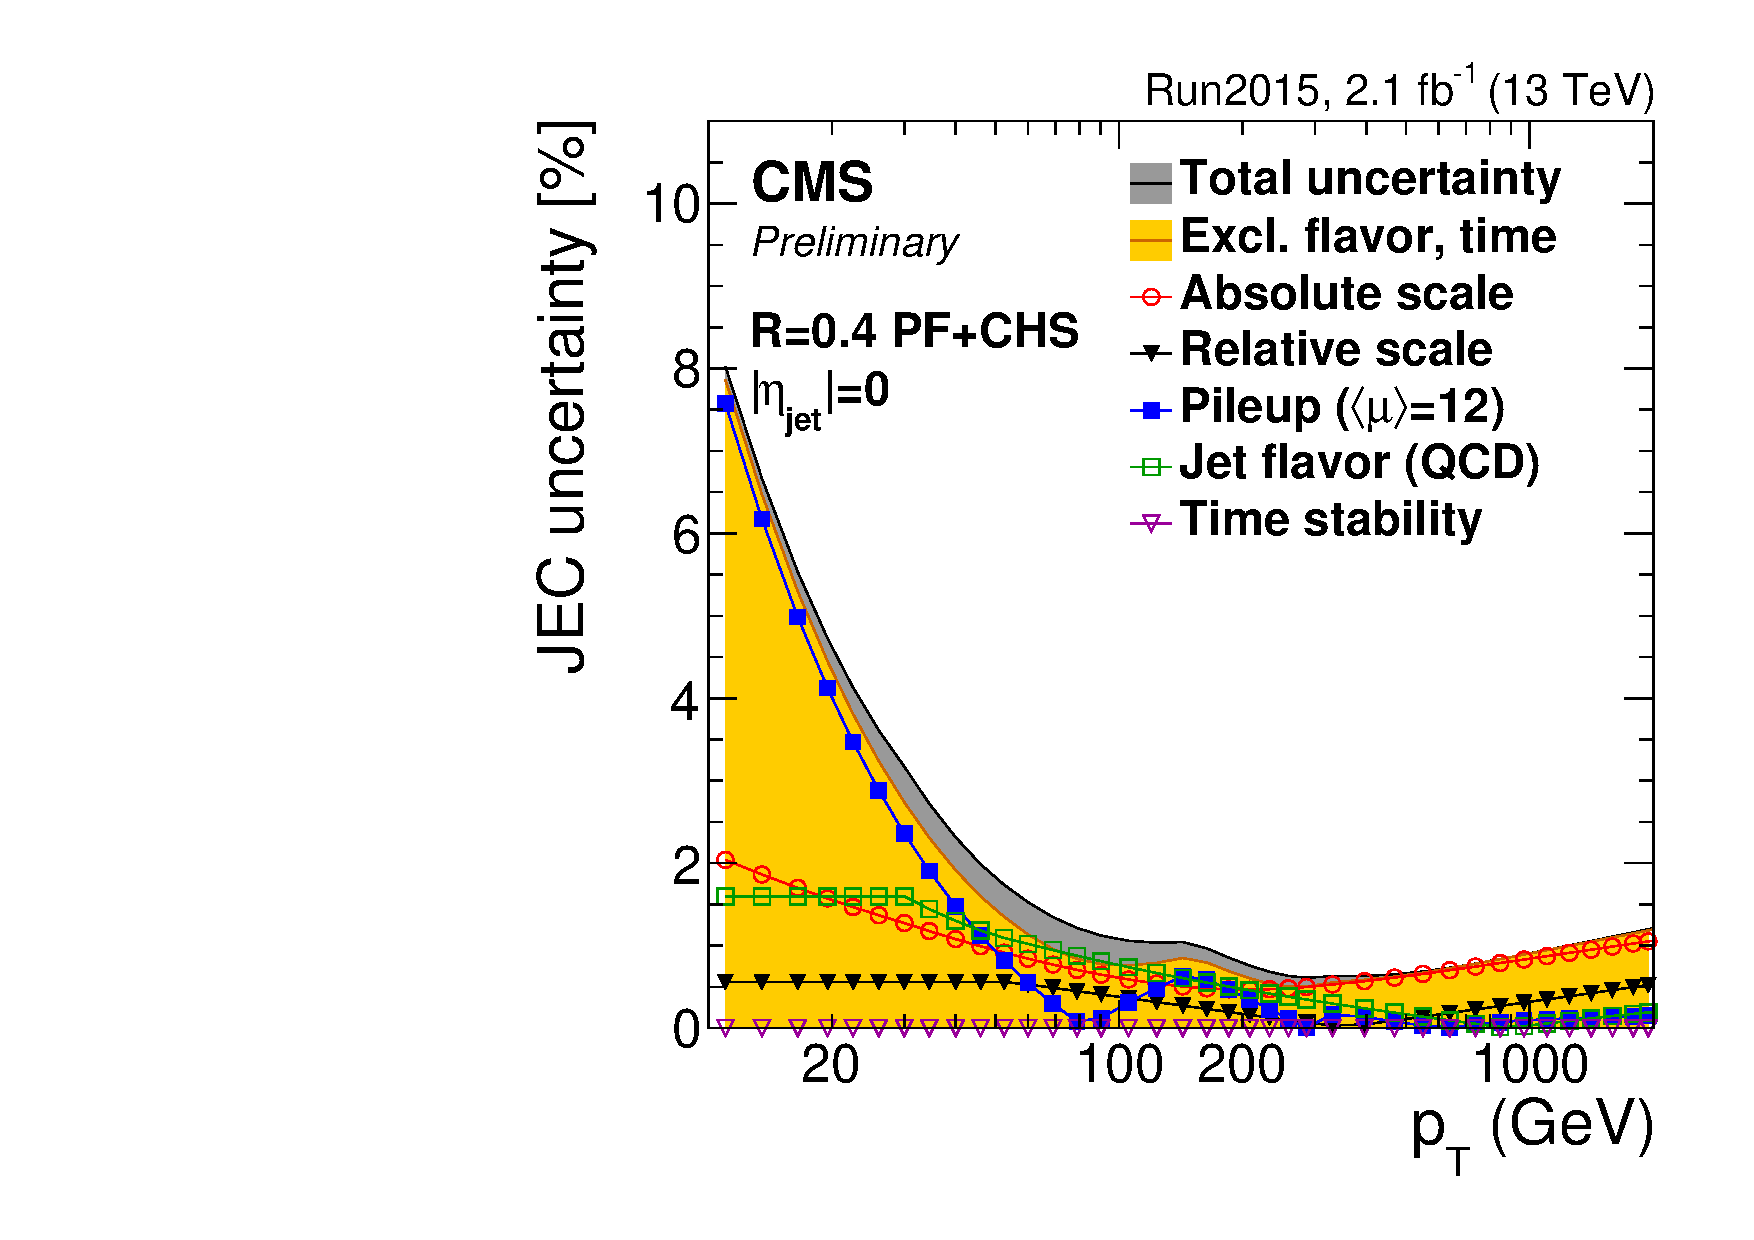
\includegraphics[width=.5\textwidth]{figures/JetPlots/JECUncert_DATA_Summary_AK4PFchs_Eta00.pdf}%
    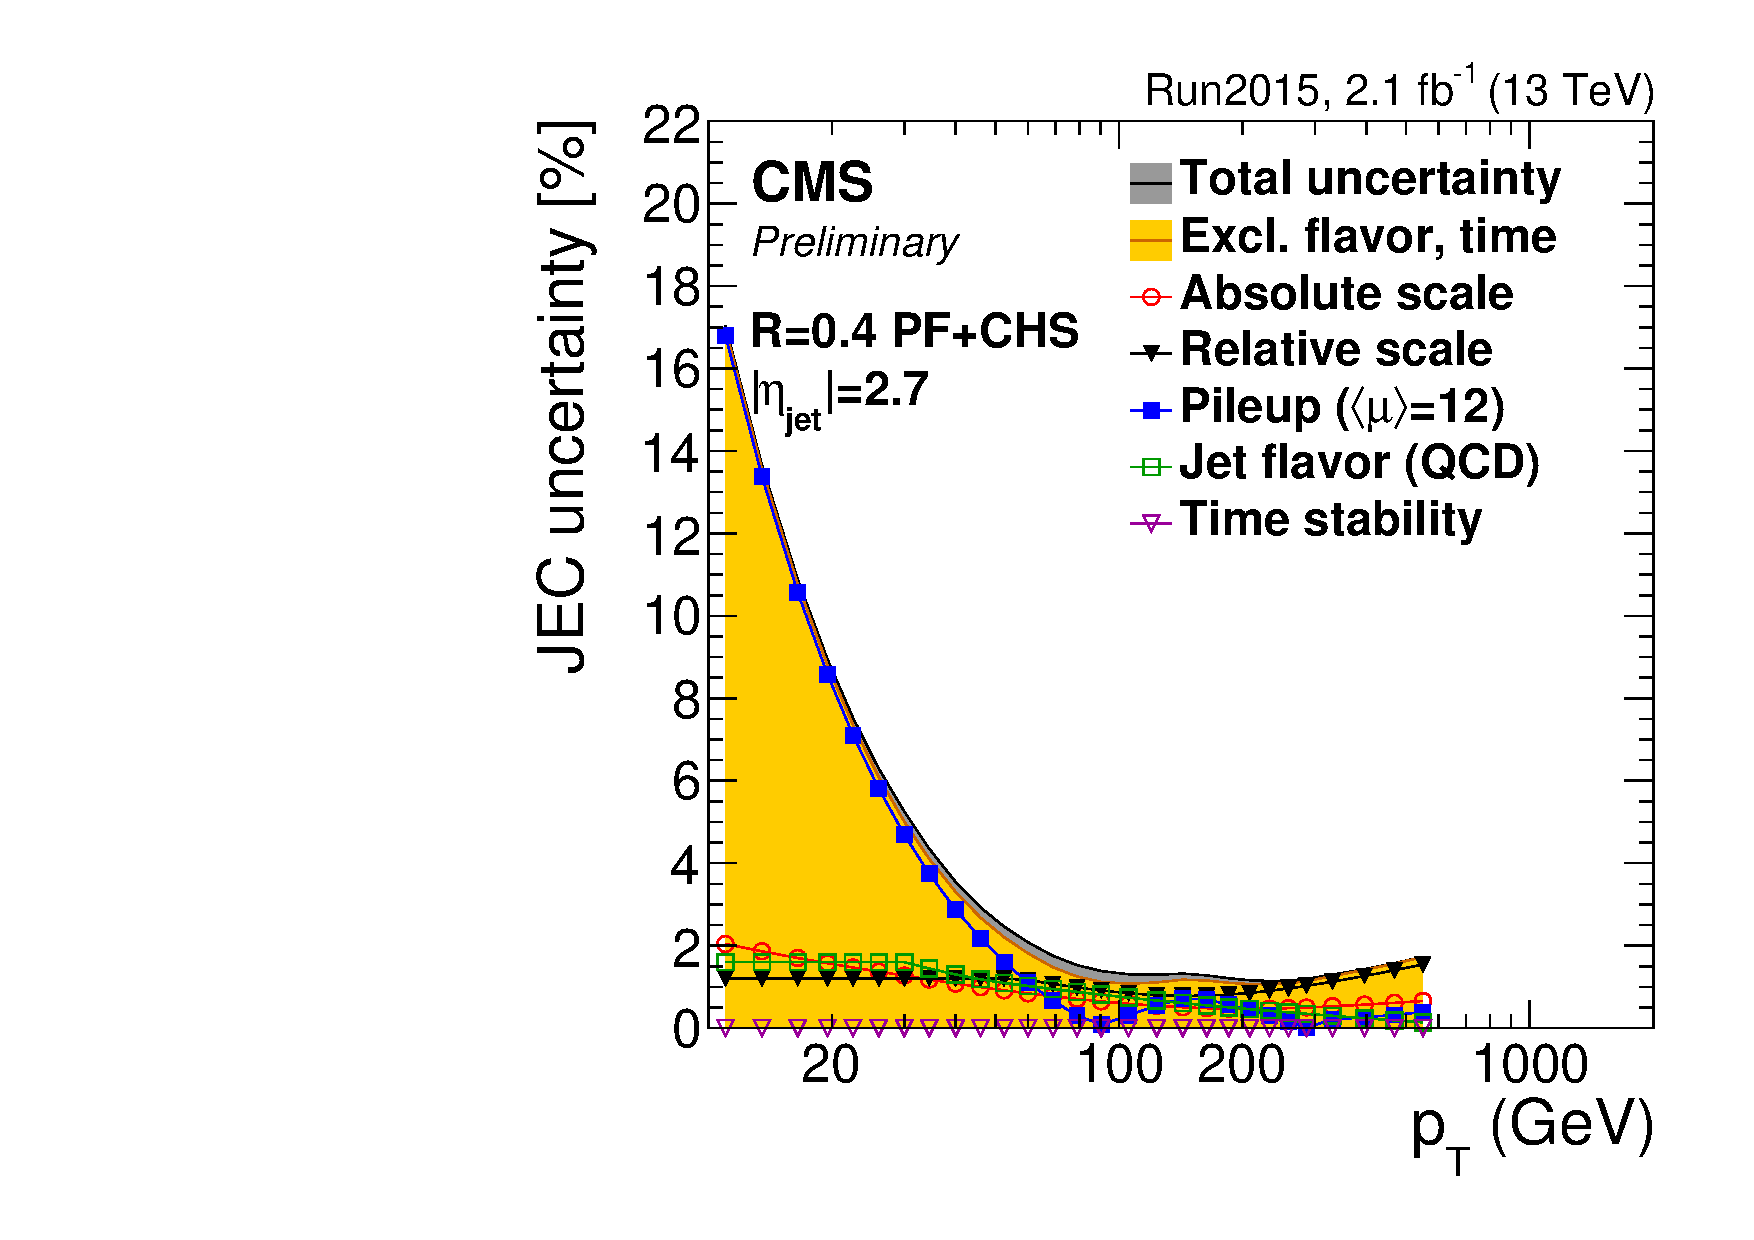
\includegraphics[width=.5\textwidth]{figures/JetPlots/JECUncert_DATA_Summary_AK4PFchs_Eta27.pdf}
\\
    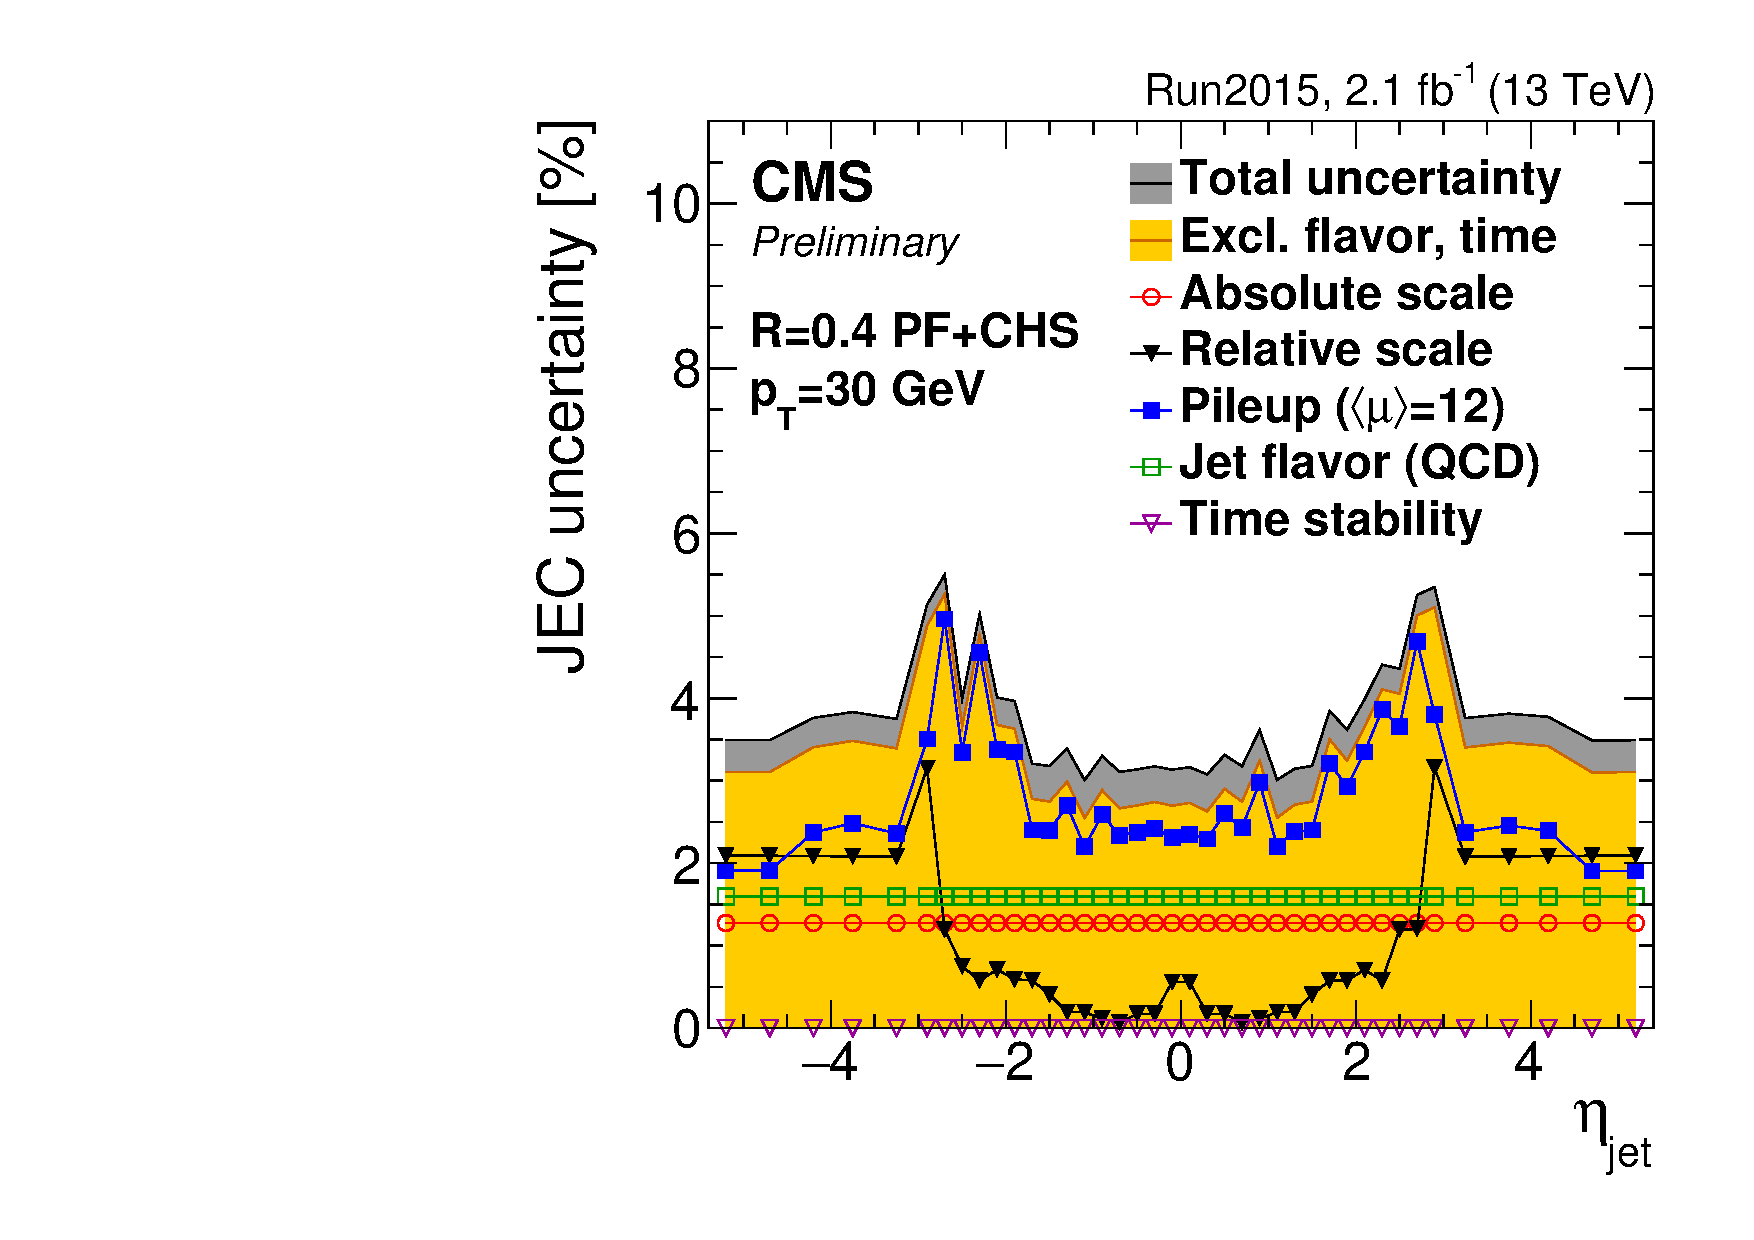
\includegraphics[width=.5\textwidth]{figures/JetPlots/JECUncert_DATA_Summary_AK4PFchs_Pt30.pdf}%
    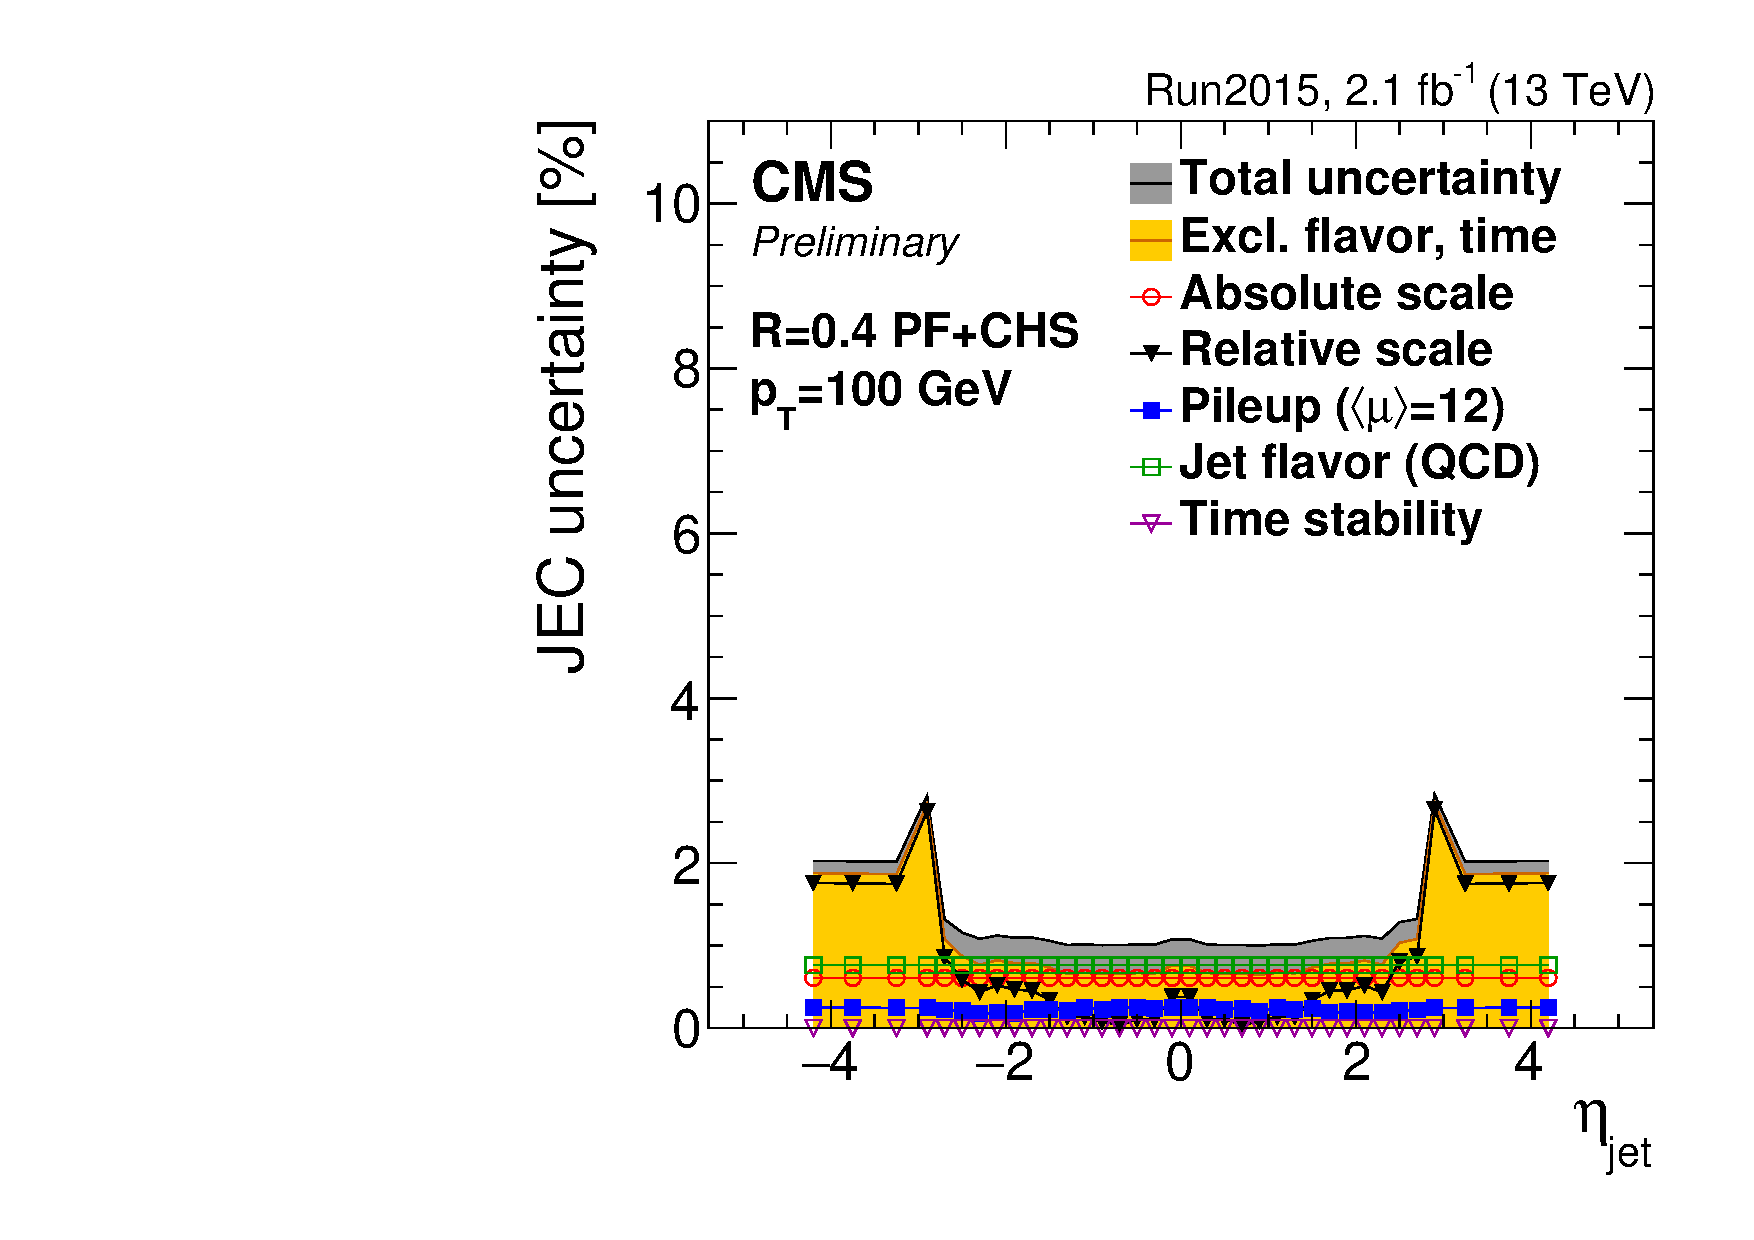
\includegraphics[width=.5\textwidth]{figures/JetPlots/JECUncert_DATA_Summary_AK4PFchs_Pt100.pdf}

  \caption{Jet energy corrections uncertainties, as a function of jet \pt (top) and $\eta$ (bottom), calculated in 2015 data. The yellow histograms report the convolution of the uncertainties applied in the analysis.}
  \label{fig:plot_JEC_unc}
\end{figure}

\noindent Each jet energy correction is determined with an uncertainty, and reported in fig.~\ref{fig:plot_JEC_unc} for 2015 data, as a function of \pt and $\eta$ of the jet. The total uncertainty for jets with \pt larger than 30 GeV (100 GeV) is smaller than 3\% (1\%) in the barrel, and up to 5\% (3\%) in the endcaps~\cite{CMS-DP-2016-020}.\\
An additional effect that must be taken in account in the analysis is the discrepancy in the jet energy resolution (JER) observed in data and in Monte Carlo samples. A smearing procedure is applied in MC simulations (described in detail in sec.~\ref{ssec:jets}), in order to restore a better agreement. Jet energy resolutions in Monte Carlo simulations are displayed in fig.~\ref{fig:plot_JER} (top), as a function of the jet \pt and the average number $\mu$ of reconstructed primary vertices, considering central (left) and forward (right) jets. The resolution is stable against the pile-up for jet \pt$>$100 GeV, and it ranges from 10\% at 100 GeV, down to 4\% at 1 TeV~\cite{CMS-DP-2016-020}. In fig.~\ref{fig:plot_JER} (bottom), data-MC smearing scale factors are reported as a function of $\eta$.
%Jets are also requested to pass loose identification criteria, in order to reject fake jets due to calorimeter noise, with more than 99\% efficiency for true jets.

\begin{figure}[!htb]
  \centering
    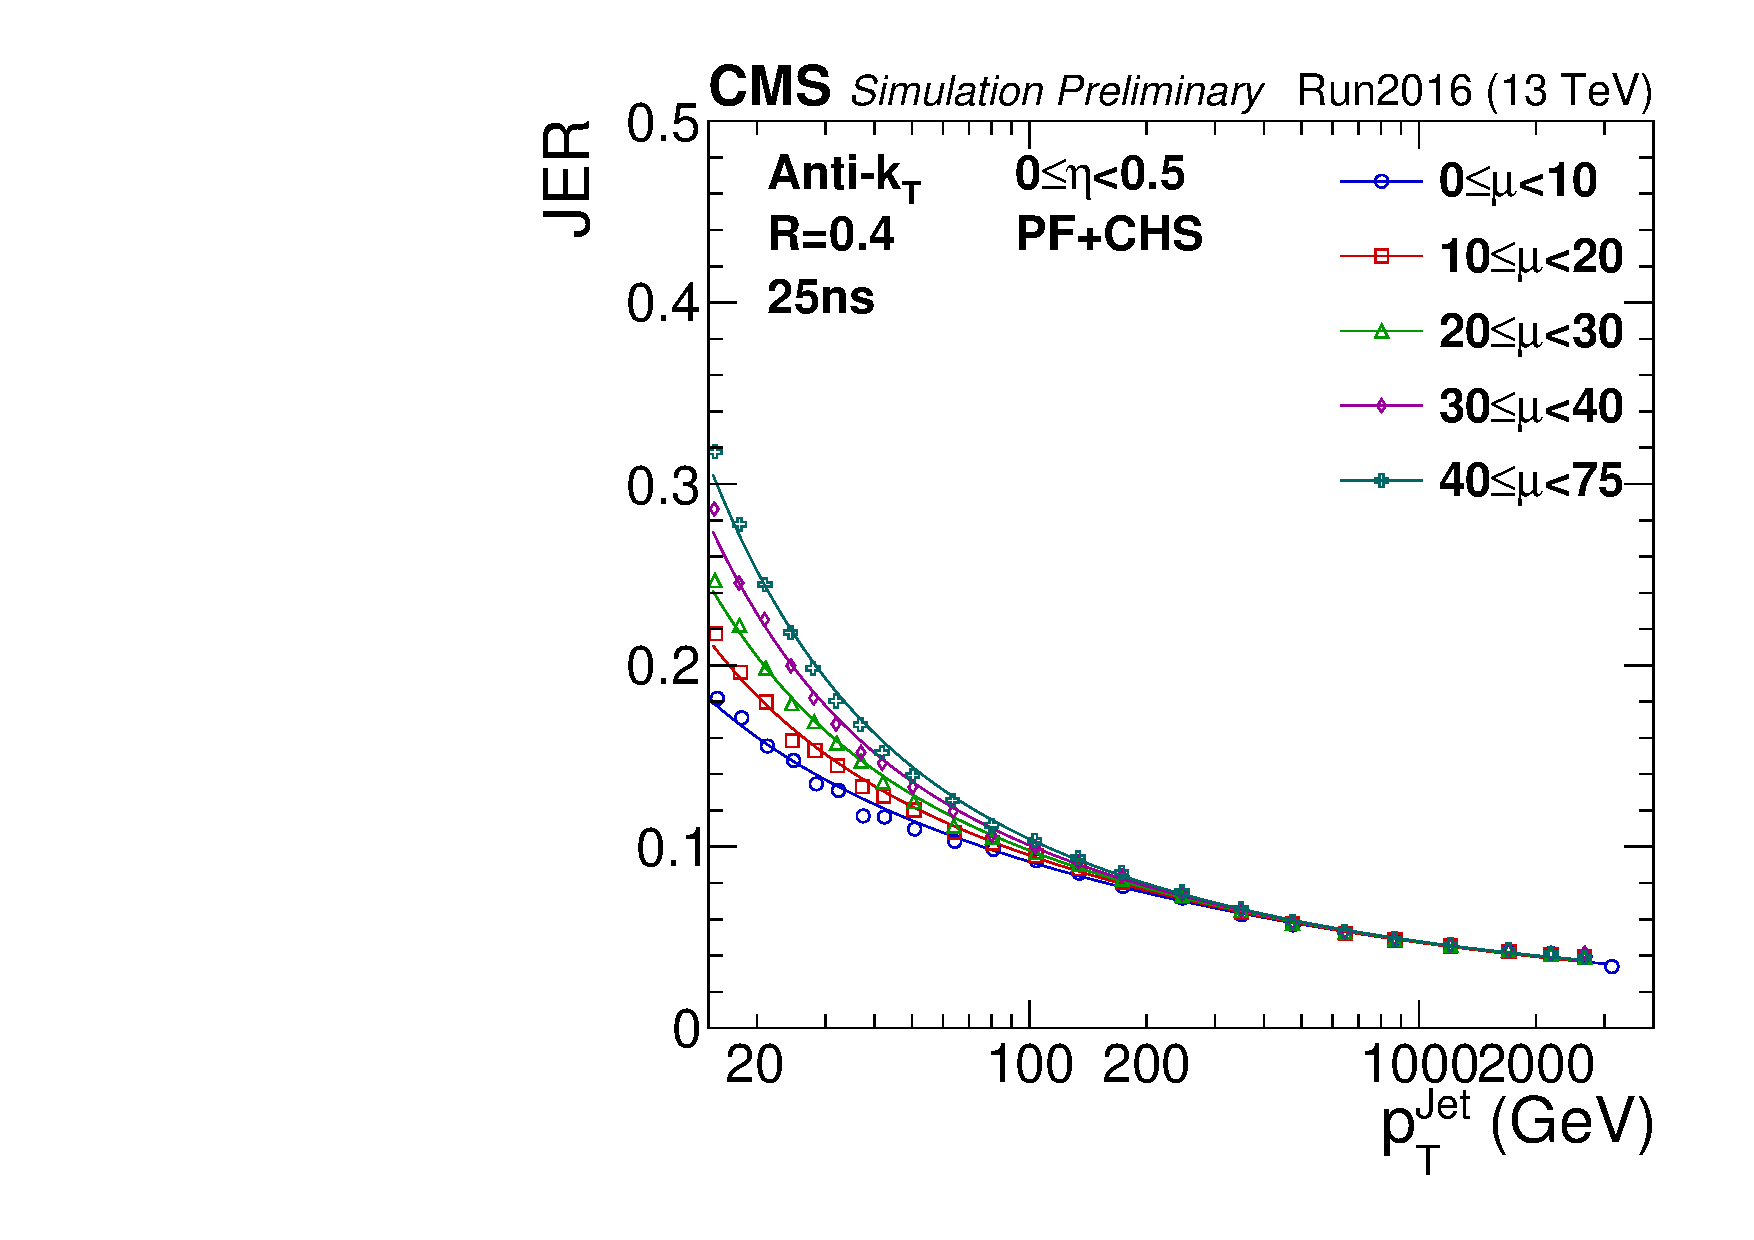
\includegraphics[width=.45\textwidth]{figures/JetPlots/RelResVsJetPt_JetEta0to0p5_Mu_80x-1.pdf}%
    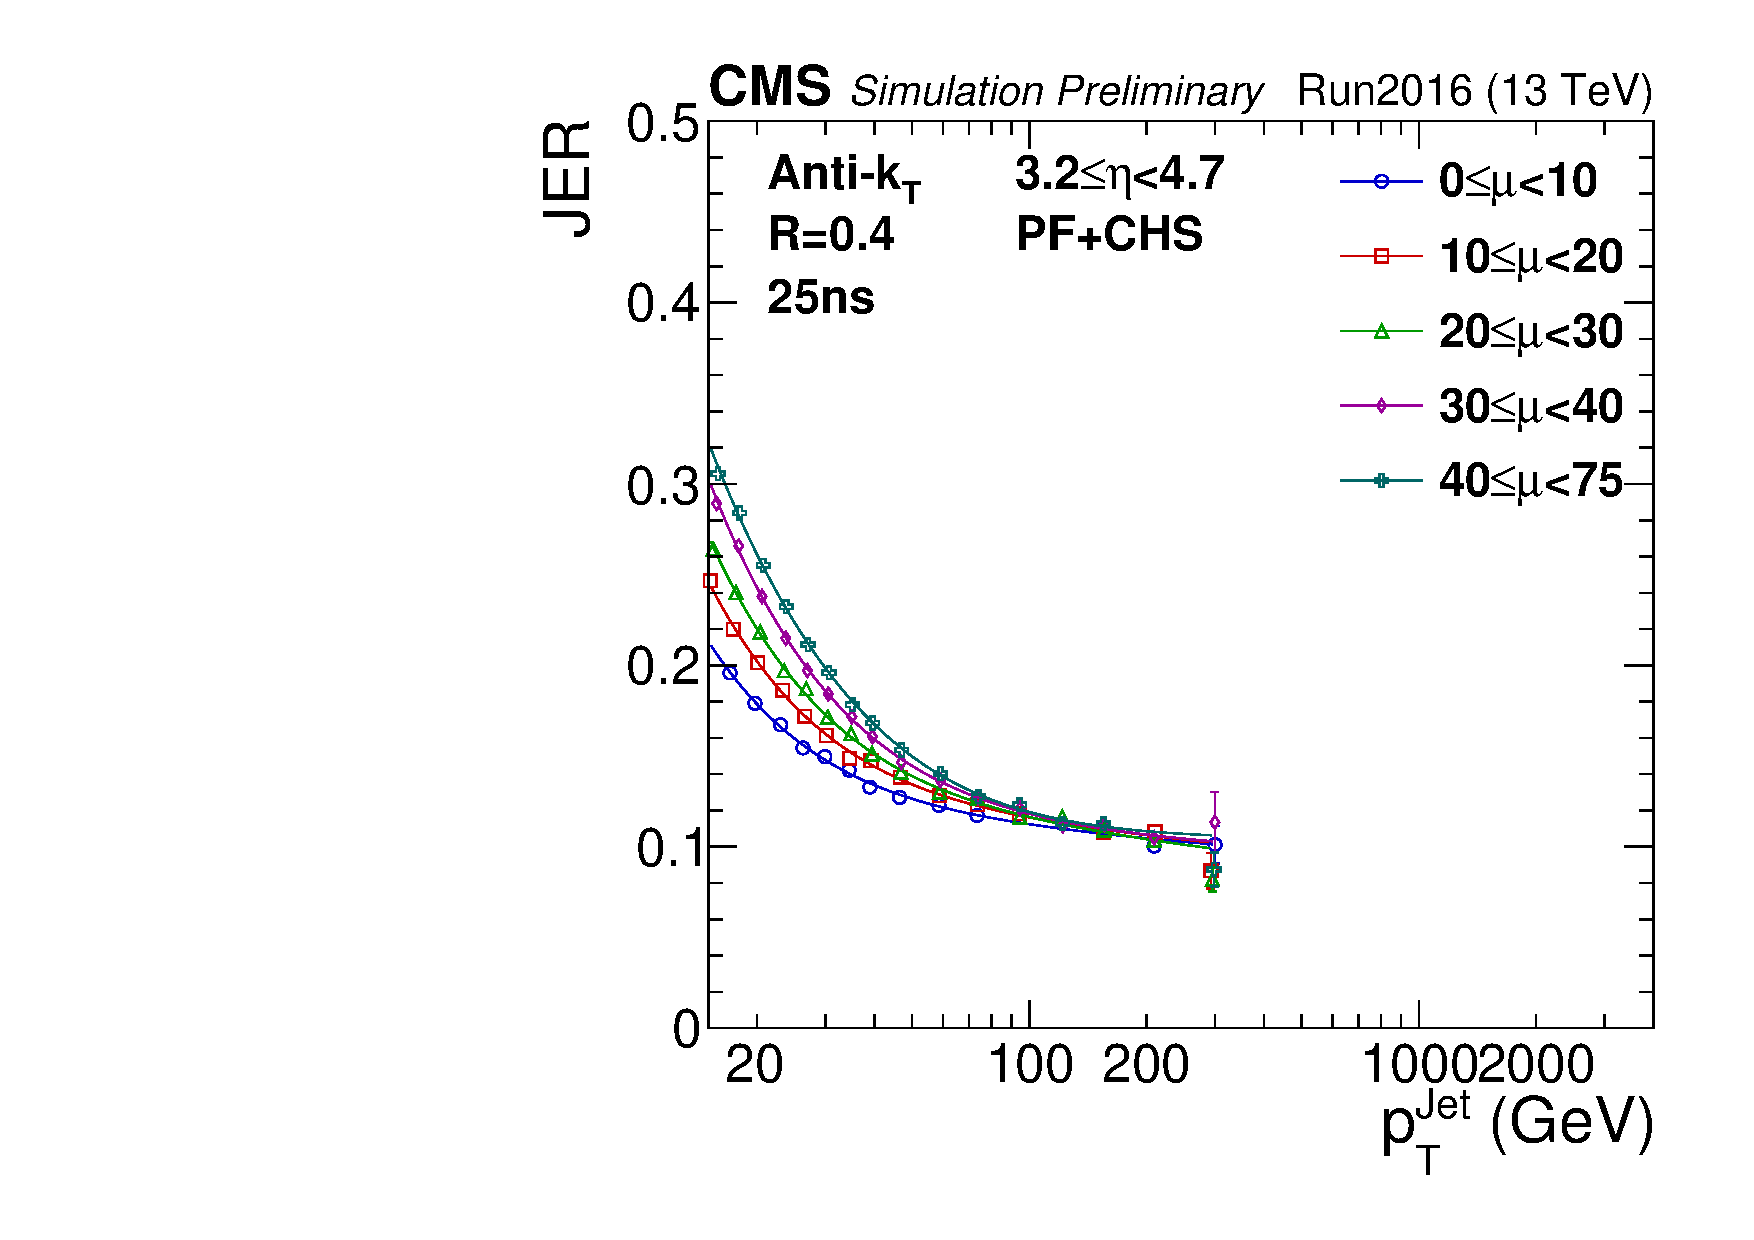
\includegraphics[width=.45\textwidth]{figures/JetPlots/RelResVsJetPt_JetEta3p2to4p7_Mu_80x-1.pdf}
\\
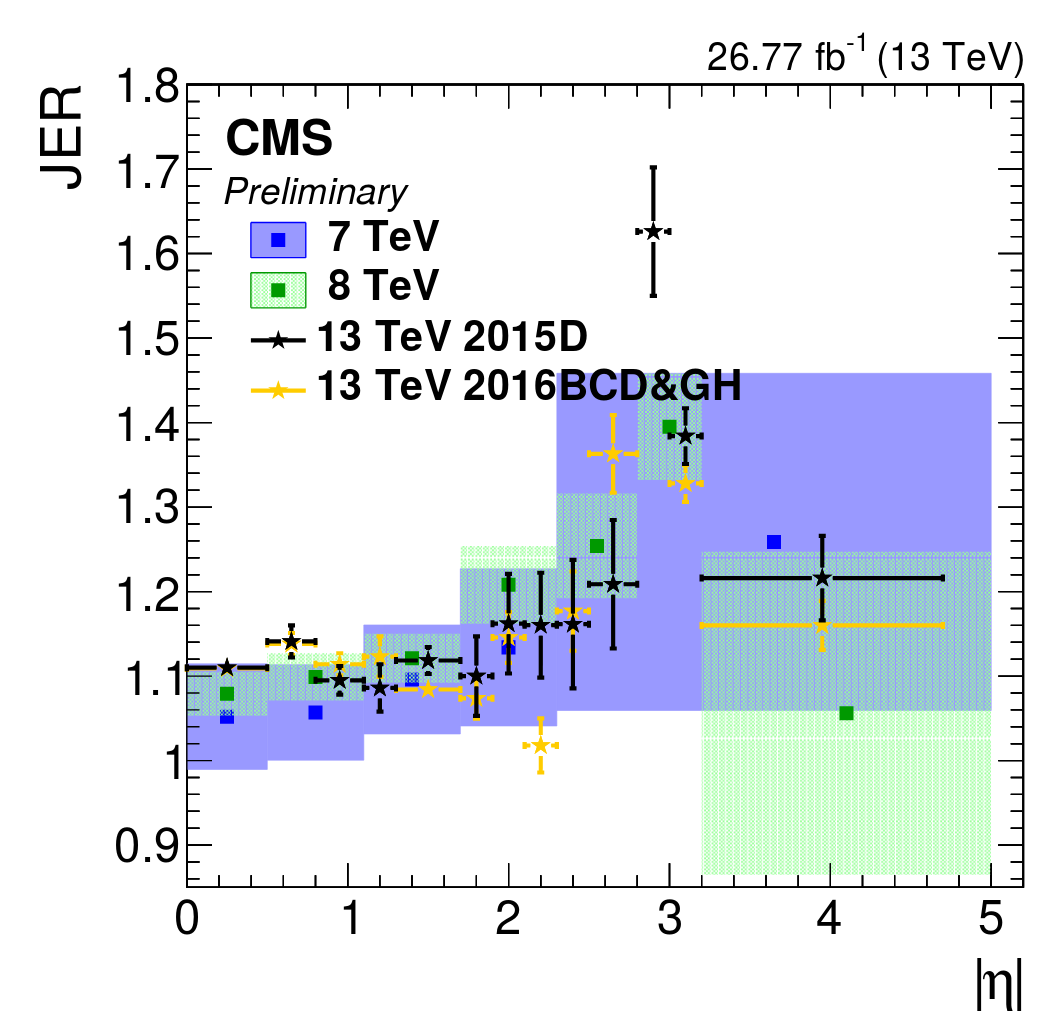
\includegraphics[width=.45\textwidth]{figures/JetPlots/JER_SF.png}
  \caption{Top: jet energy resolution in MC simulations, as a function of the jet \pt. Different curves represent a different average number of primary vertices per event ($\mu$). Bottom: data-MC scale factors, as a function of the jet $\eta$, measured in 2016 data (yellow dots).}
  \label{fig:plot_JER}
\end{figure}

%Several levels of jet energy corrections are applied to the momentum of the clustered (raw) jets in order to obtain the energy value that is closer to the true energy of the initial parton


%Charged and neutral hadrons deposit their energy in the hadron calorimeter (HCAL) made
%of brass and scintillators, installed inside the coil and surrounding the ECAL, with a similar
%pseudo-rapidity coverage. The granularity of the HCAL is 25 times coarser than that of
%the ECAL, which would not allow charged and neutral hadrons to be spatially separated in
%jets with a transverse momentum much above 100 GeV/c. The hadron energy resolution in
%the combined ECAL–HCAL system is, however, of the order of 10\% at 100 GeV. This resolution
%allows neutral hadrons to be detected as an energy excess on top of the energy deposited
%by the charged hadrons pointing to the same calorimeter cells. The charged hadrons are reconstructed
%with the superior angular and energy resolutions of the tracker. Particles with
%pseudo-rapidities between 3.0 and 5.0 are more coarsely measured with an additional forward
%calorimeter (HF), placed 11 m from the interaction point.
%[PF paper]

\subsubsection{Tau reconstruction}
\noindent Tau leptons have a very small lifetime ($\sim 3 \times 10^{-13}$ s), hence they decay before reaching the pixel detector and they can only be reconstructed through their decay products. Approximatively 60\% of the times, $\tau$ leptons decay in hadrons, hence they are reconstructed as small collimated jets in the CMS detector. The main decay modes of the hadronic tau, $\tau_h$, are one or three charged mesons (mainly $\pi^{\pm}$), also in association with a $\pi^0$ decaying in a couple of photons, and a $\tau$ neutrino. Hence, photons and charged hadrons are the main ingredients of dedicated algorithms to perform the $\tau_h$ reconstruction and identification, in order to distinguish them from quark and gluon-initiated jets. The main CMS $\tau_h$ reconstruction algorithm, Hadron Plus Strips (HPS)~\cite{Chatrchyan:2012zz}, is particle flow based. HPS builds the tau candidate from a PF jet, clustered with the anti-\kt algorithm with $R_0 = 0.5$, and it reconstructs the $\pi^0 \rightarrow \gamma \gamma$ decays within the jet cone, by taking into account the photon conversions in the silicon detector. The exploitation of the PF informations is such that the HPS algorithm shows stable performances in the reconstruction of the $\tau_h$ energy as a function of the energy itself. The $\tau_h$ candidate is required to be isolated, namely no energy deposits other than the $\tau$ decay products should be present in the tau cone. Depending on the low threshold set to consider the surrounding particles as included in the cone, different isolation working points can be defined. With the looser working point, the probability of mis-identifying a quark or gluon jet as a tau is around 1\%~\cite{Chatrchyan:2012zz}.

\subsubsection{b-jets tagging}
\indent The bottom quark plays a fundamental role in numerous standard model processes, \textit{i.e.} the physics related to the top quark (that decays into a W and a b-quark with a branching fraction of 100\%) and the Higgs boson (decaying into $b \bar{b}$ with a branching fraction $\sim$60\%). Many algorithms have been exploited by the CMS collaboration, with the aim of distinguishing a b-quark initiated jet and jets originating from light quarks or gluons~\cite{CMS-PAS-BTV-15-001}. The most remarkable feature of the b-quark is the long lifetime ($\sim$~1.5 ps), that has the experimental consequence of a displaced decay (few mm) with respect to the primary vertex. The direct leptonic decays of the b-quark (into $\mu$ and $e$) or the cascade leptonic decays involving c-quarks give an additional handle to its identification.\\
Given the high spatial resolution of the silicon detector, track reconstruction is a key point of the b-tagging procedure. Tracks inside a jet candidate must satisfy criteria related not only to their quality but also on their distance from the interaction point. The track impact parameter is the distance between the primary vertex and the coordinate of closest approach. Tracks that are too far from the interaction point are discarded, in order to suppress the pile-up contributions. The Combine Secondary Vertex (CSV) algorithm~\cite{Chatrchyan:2012jua} sorts jet candidates in categories, based on the number of reconstructed secondary vertices (one reconstructed secondary vertex, no secondary vertices but two tracks with high impact parameters, and the remaining cases). A multivariate approach allows to train the algorithm over the categories, considering as discriminating variables both tracking informations (numbers and properties of the tracks) and their relations with the secondary vertex reconstruction (impact parameters; angular, linear, 2D and 3D distances of the vertex from the tracks and the jet axis; invariant mass of the charged particles associated to the secondary vertex).\\
By tuning the selections, working points with different efficiencies have been set. The loose working point, used in this analysis, has a 90\% signal efficiency and a 40\% mis-identification rate. The b-tagging efficiency is different in data and in simulations. Multiplicative scale factors are calculated in events enriched in b-quark jets.\\
%It is known that b-tagging efficiency is not the same in data and MC. In order to take into account this shortcoming, the BTV POG provides collections of b-tagging scale factors for b-jets and mistagged light jets, measured for different physics processes, for the supported tagging algorithms and the three standard working points [42]. A weight is calculated on a per-event basis as a function of the b-tagging status and the flavour of the hadron that initiated the jet in the event [40].

\subsubsection{Missing transverse energy reconstruction}
\label{ssec:met_description}
Neutrinos can interact with the other particles only via the electroweak interactions; hence, when a neutrino is produced in the proton-proton collisions, it passes through the CMS experiment, undetected. Its only experimental signature is the momentum imbalance (\met) in the transverse plane $(r, \varphi)$. The magnitude of \met vector is also called missing transverse energy, \MET. Given its definition, it is evident that \MET is a delicate variable to deal with, since it depends on all the other objects, on their imperfect measurements, on the detector noise and the pile-up events.\\
The PF \MET is the negative sum of the transverse momenta of the PF candidates reconstructed in the event. Inefficiencies in the tracker reconstruction and non-linear responses of the calorimeters can be corrected by propagating the jet energy corrections to \met~\cite{CMS:2016ljj}:
\begin{equation}
\vec{p}_T^{\text{miss,corr}} = \vec{p}_T^{\text{miss}} - \sum_{j \in \text{jets}} \left( \vec{p}_{T,j}^{\text{corr}} - \vec{p}_{T,j}^{\text{raw}}\right),
\label{eq:met_typeI}
\end{equation}
where "corr" ("raw") is related to corrected (raw) \pt of the considered jet. This correction is known as the "Type-I" correction to \MET. Jets included in the calculation are AK4 with CHS algorithm applied to remove the pile-up contribution, they must have $p_T>15$ GeV and less than 90\% of their energy deposited in the electromagnetic calorimeter. If a muon lies in the jet cone, it is subtracted from the jet and added after the $p_T$ correction. A similar correction is performed to correct \met at trigger level; in this case, a jet \pt threshold of 35 GeV is chosen.\\
The \MET uncertainty depends on the topology of the final state. It is calculated per-event by factorizing \met in components: electrons, photons, muons, taus, jets, jets with \pt$<$10 GeV and all the remaining PF candidates that are not clustered inside jets, called unclustered energy. The momentum of every object is varied within its uncertainties (namely, the energy scale and resolution), and the effects are propagated to \met. The most significant contributions in the unclustered energy is due to neutral PF hadrons and hadrons reconstructed in the forward hadronic calorimeter. The effects related to jet energy scale and unclustered energy scale are measured on simulation, in events with a top and an anti-top quarks, and amounts to 5\% and 30\% respectively~\cite{CMS:2016ljj}.\\

\begin{figure}[!htb]
  \centering
    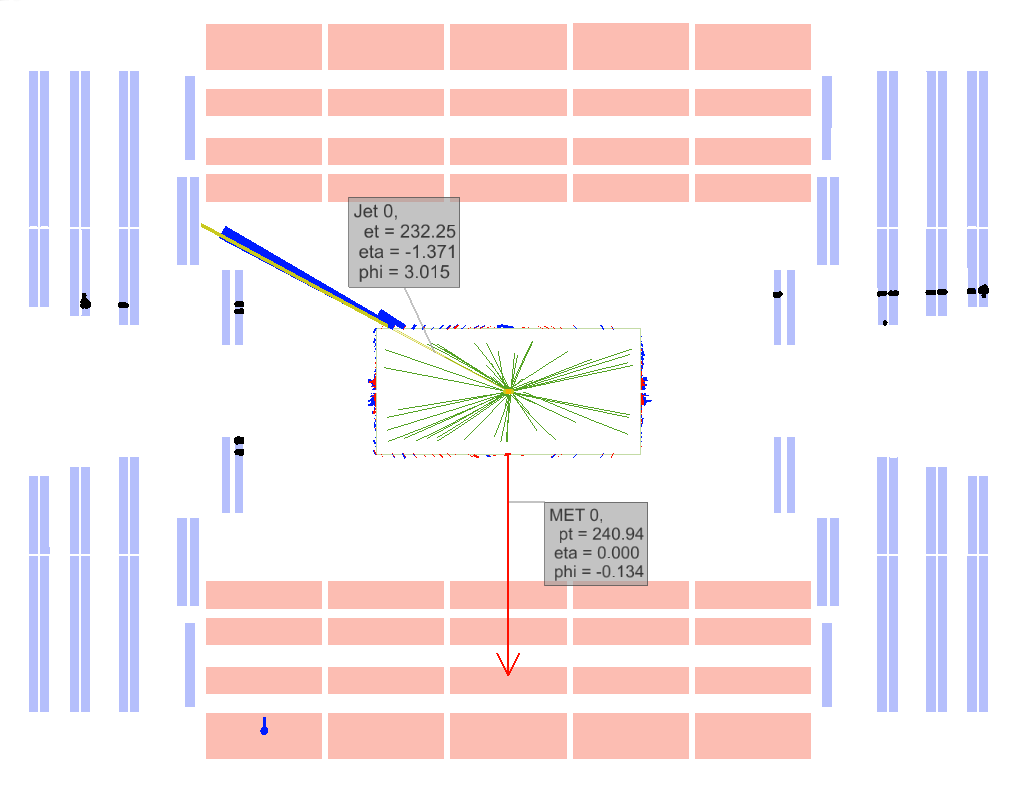
\includegraphics[width=.45\textwidth]{figures/MetPlots/BeamHalo_event_display.png}%
    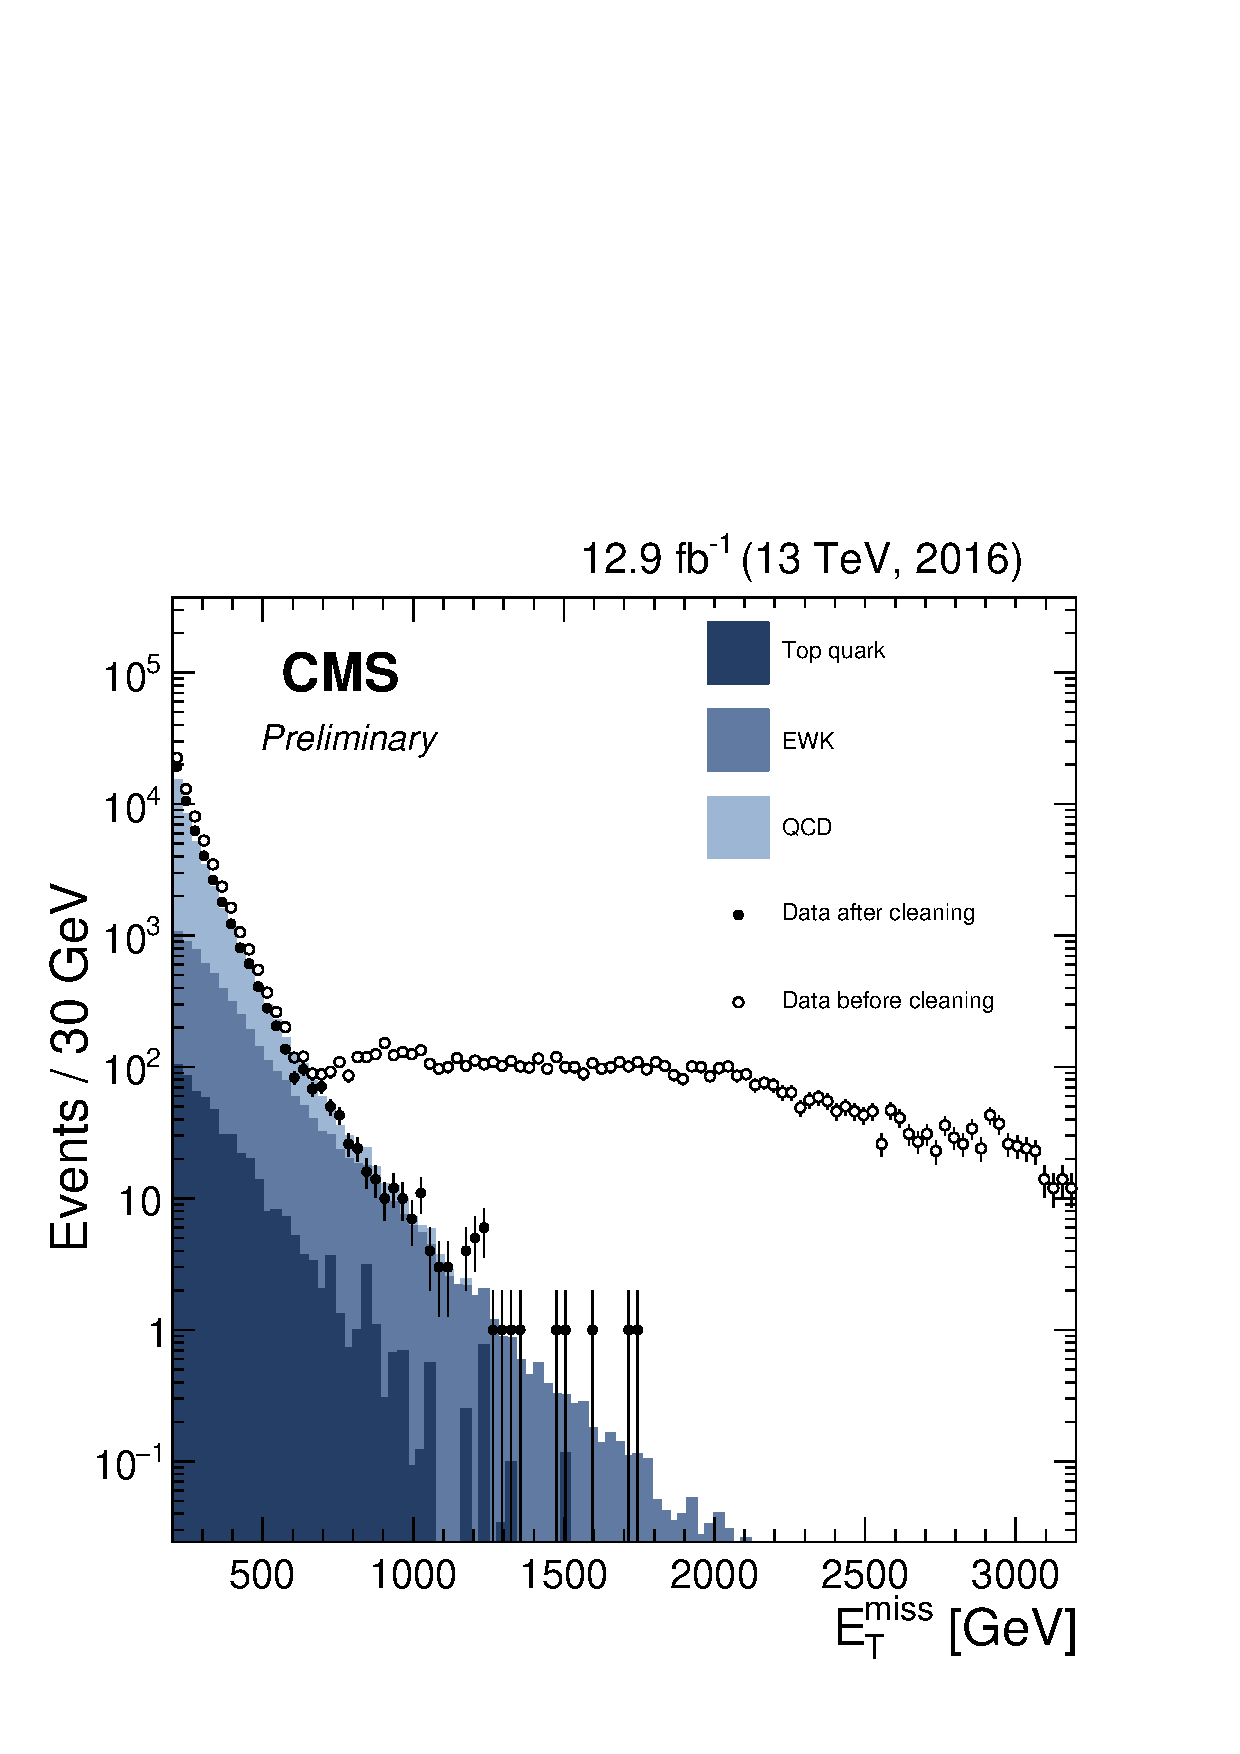
\includegraphics[width=.35\textwidth]{figures/MetPlots/Filters.pdf}

  \caption{Left: event display of beam halo particles hitting the CSC detector. Right: comparison of data and simulations (histograms) when di-jet events are selected, before (open markers) and after (filled markers) anomalous \MET cleaning algorithms have been applied on data.}
  \label{fig:met_filters}
\end{figure}

\noindent Many instrumental effects can give rise to anomalous \MET determination: they have been studied in detail during Run1~\cite{Chatrchyan:2011tn,CMS:vgm} and Run2~\cite{CMS:2016ljj}, and they are mainly caused by ECAL and HCAL. In ECAL, anomalous \met is caused by particles hitting the sensors of the photodetectors, or by beam halo particles (namely, particles produced in spurious proton interactions before reaching the interaction point in the detector) showering inside the calorimeter, or by losses due to ECAL dead cells. An event display representing beam halo muons hitting the CSC detector is shown in fig.~\ref{fig:met_filters} (top). In HCAL, spurious \met can be related to noise in the hybrid photodiodes and readout frontend. In HF, missing \pt can be related to particles lost in the light guides and photomultipliers. Additional anomalous \MET can be produced by low quality muon tracks, that are not linked to segments reconstructed in the muon chambers by the PF algorithm. These tracks are then classified as charged hadrons, taken into account in the \met calculation, and result into a large amount of fake \MET. Dedicated algorithms have been designed to identify and reject events with anomalous \MET, and they are consistently applied on data and simulations. In fig.~\ref{fig:met_filters} (right), Monte Carlo simulations (coloured histograms) are compared to data before the algorithms removing the anomalous \MET have been applied (open markers) and after the cleaning (filled markers): the spurious high-\met tail has been suppressed.

\begin{figure}[!htb]
  \centering
    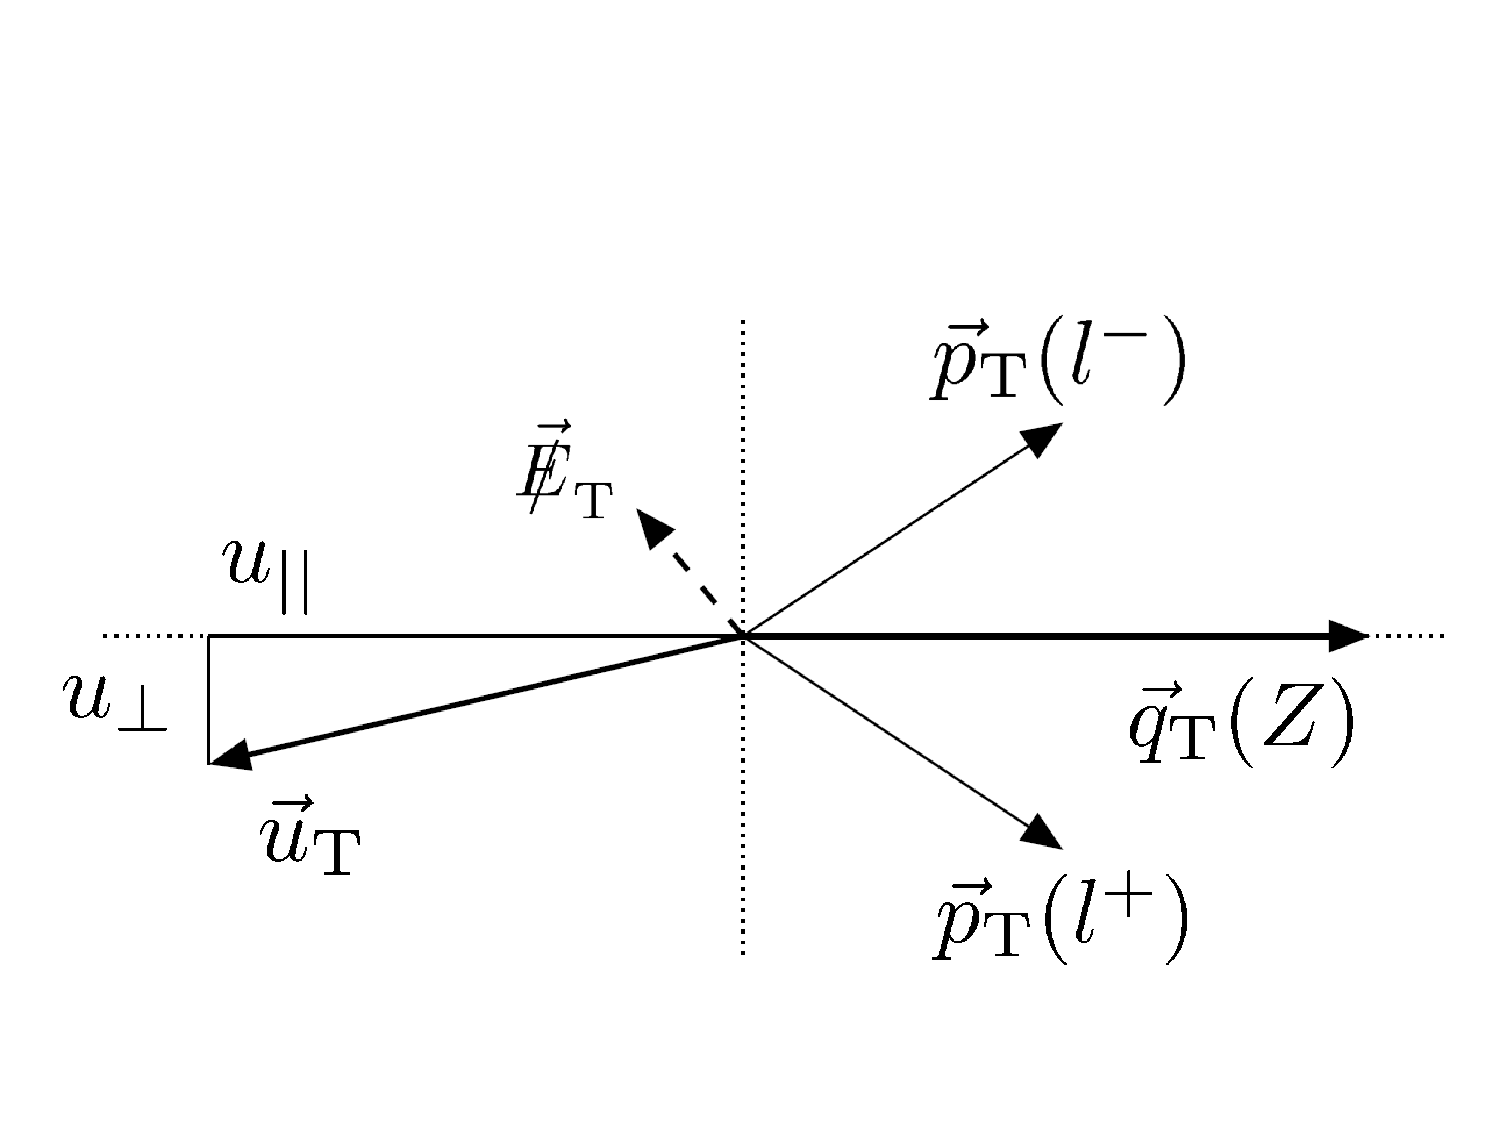
\includegraphics[width=.35\textwidth]{figures/MetPlots/u_comp_Z.png}%
    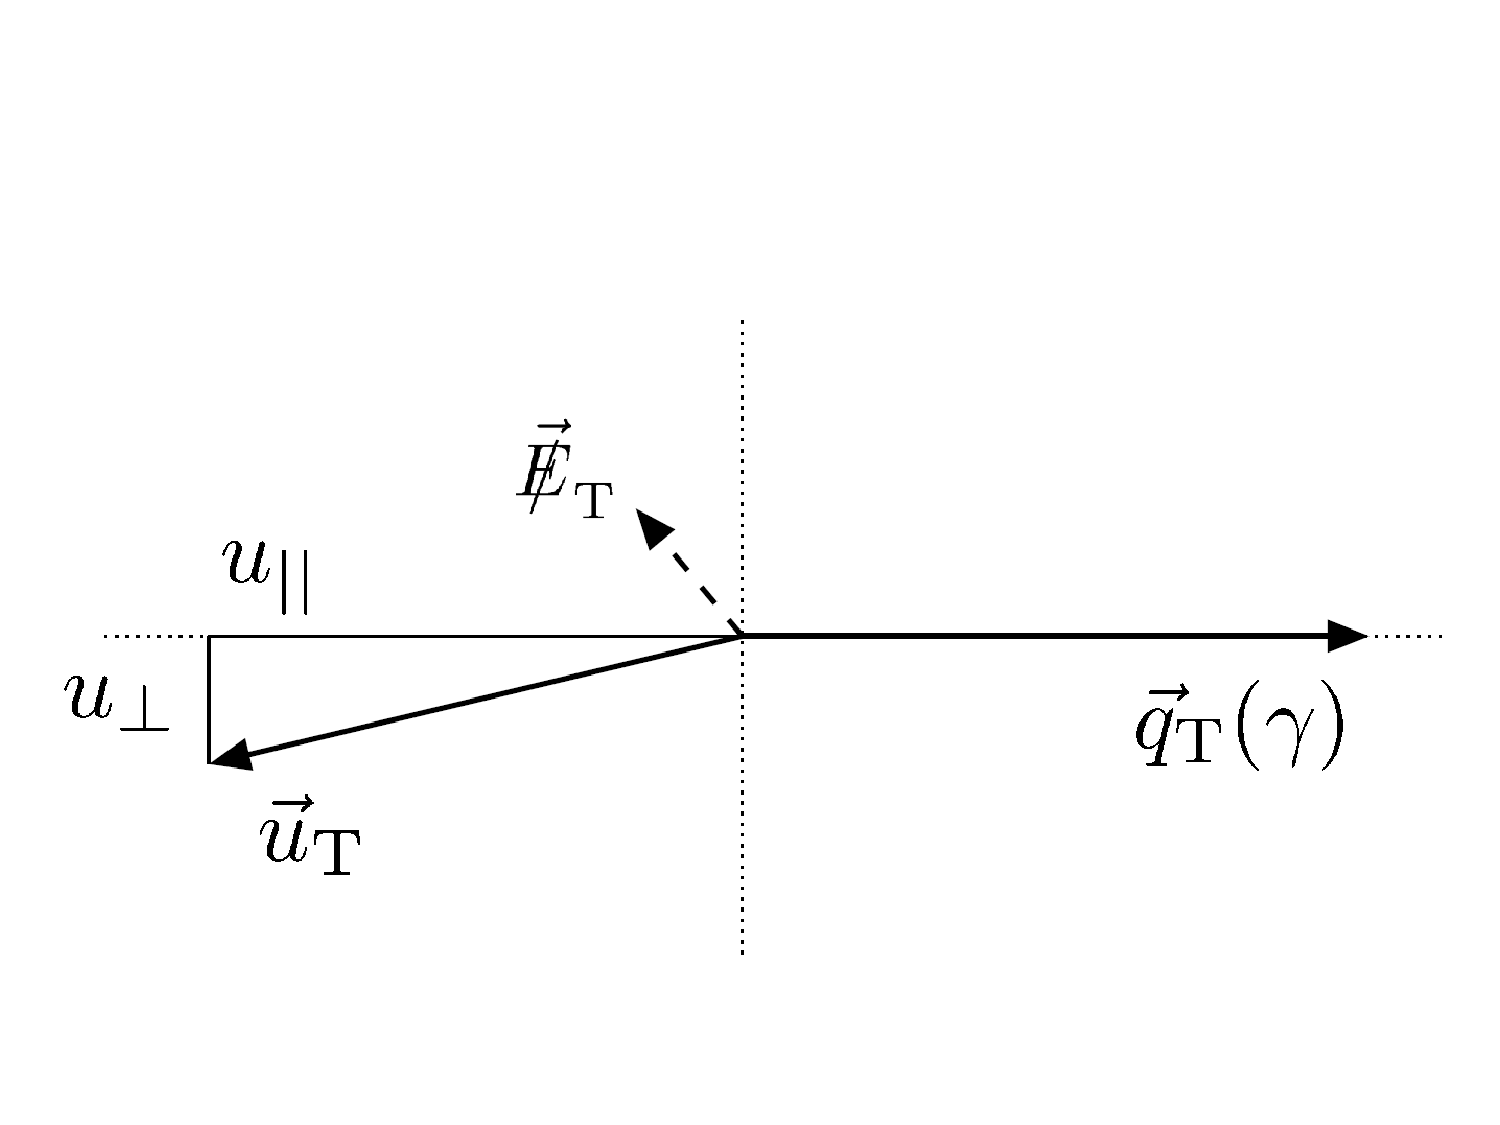
\includegraphics[width=.35\textwidth]{figures/MetPlots/u_comp_gamma.png}

  \caption{Left (Right): kinematics of $Z \rightarrow \ell \ell$ (photon) events in the $(r, \varphi)$ plane; $\vec{u}_T$ is the hadronic recoil, $\vec{q}_T$ is the transverse momentum of the considered boson.}
  \label{fig:recoil}
\end{figure}

\noindent Performance of \MET reconstruction are studied in events with a leptonic decay of a Z boson (in two muons or in two electrons) or an isolated photon. The distributions of \MET are shown in fig.~\ref{fig:recoil_distribution}, separately for the three event categories. The hadronic recoil $\vec{u}_T$ is defined in the transverse plane as the vectorial sum of all the particle transverse momenta, except the momentum $\vec{q}_T$ of the vector boson considered (Z or $\gamma$). From the momentum conservation, the following relation holds:
\begin{equation}
\vec{q}_T + \met + \vec{u}_T = 0.
\label{eq:recoil_def}
\end{equation}

\begin{figure}[!htb]
  \centering
    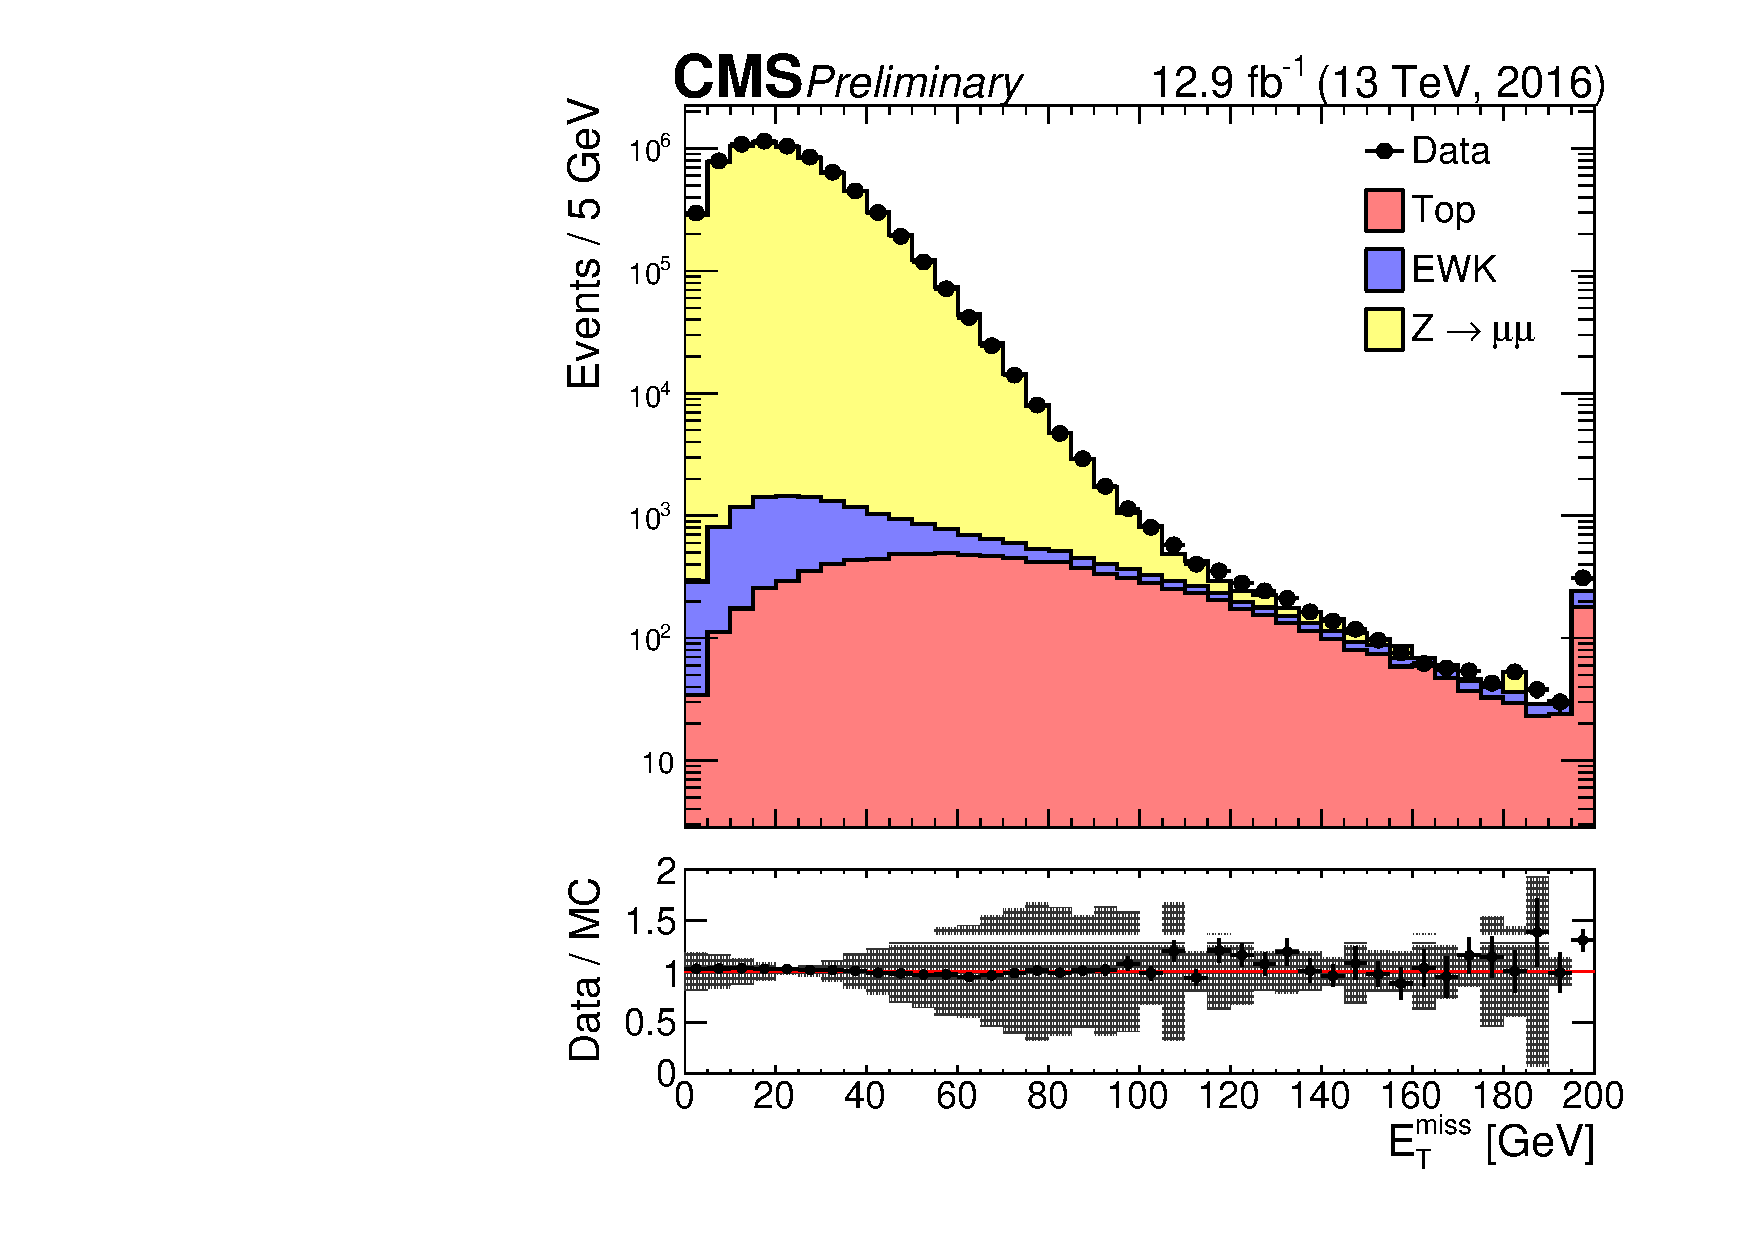
\includegraphics[width=.33\textwidth]{figures/MetPlots/distr_mu.pdf}%
    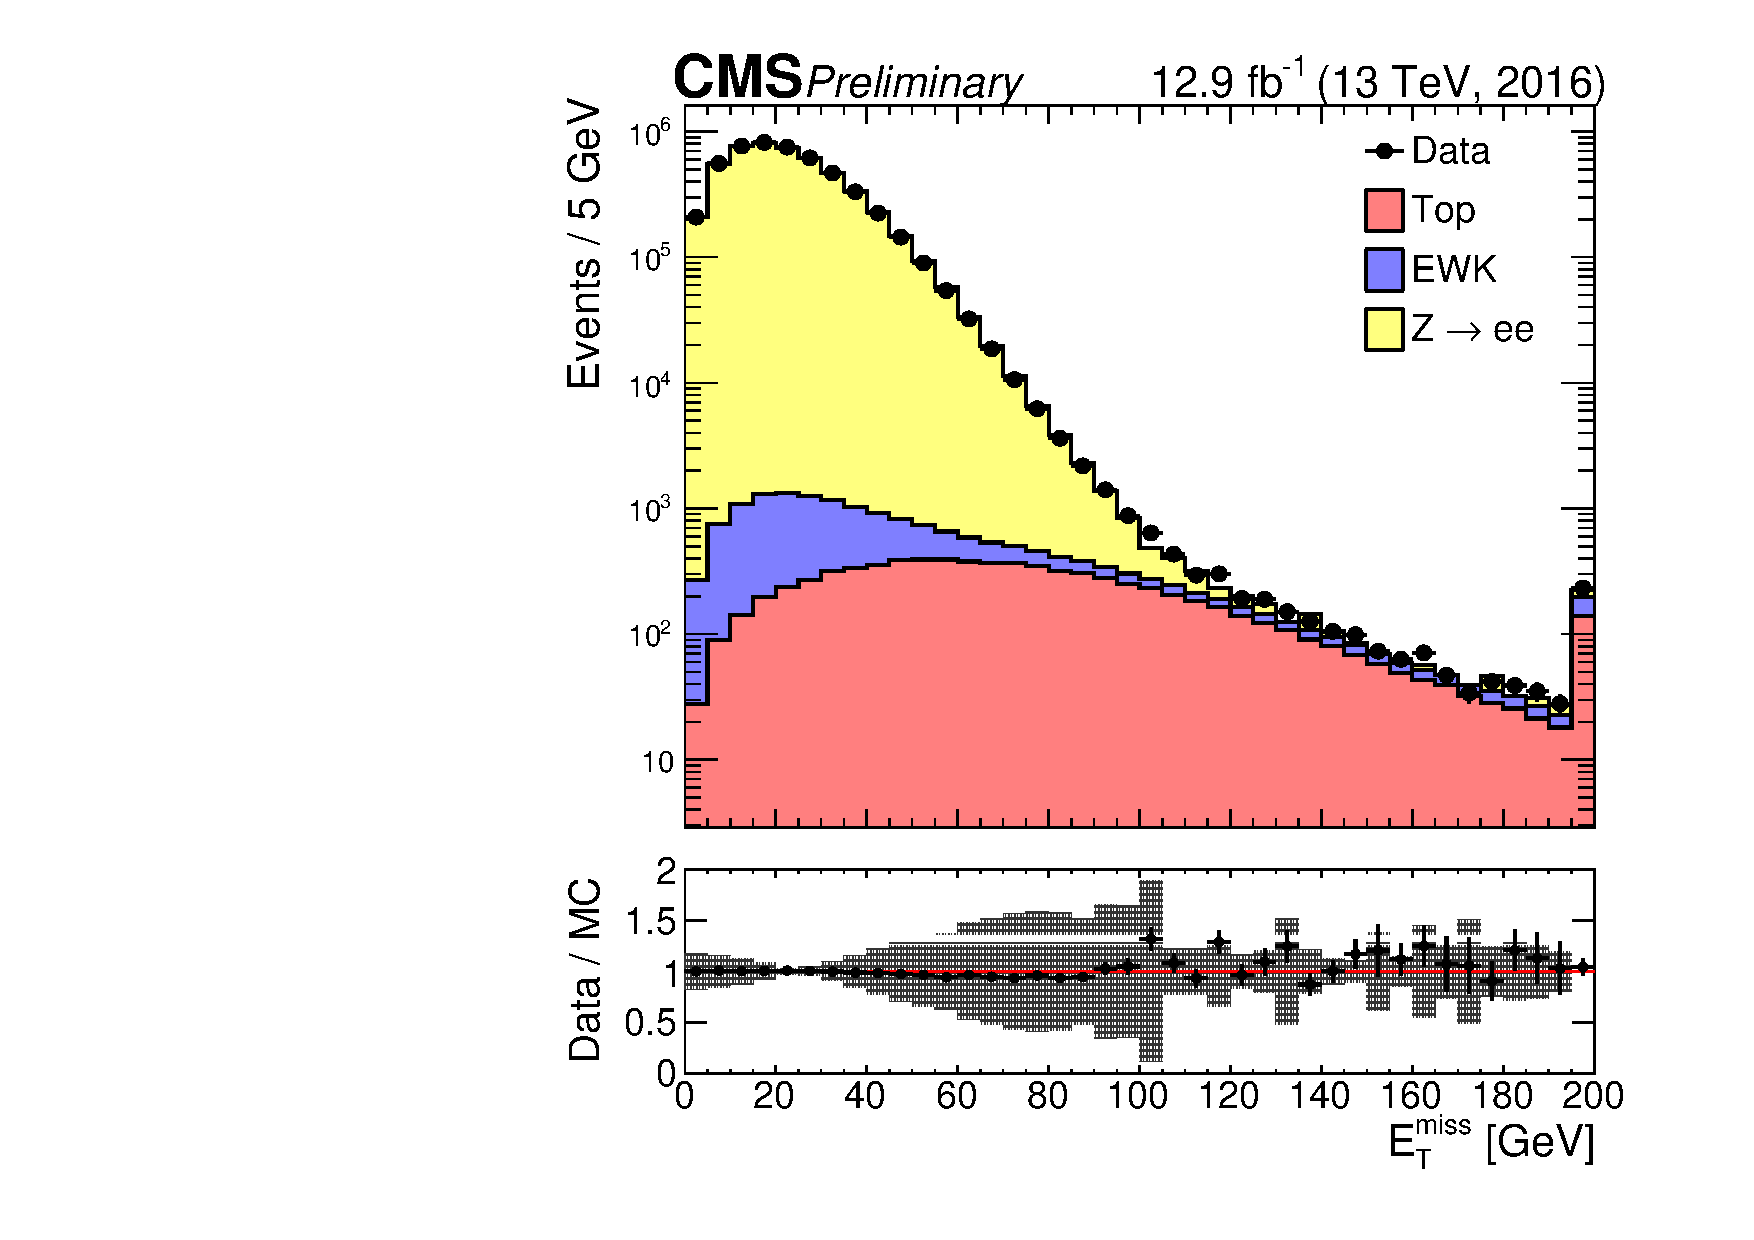
\includegraphics[width=.33\textwidth]{figures/MetPlots/distr_ele.pdf}%
    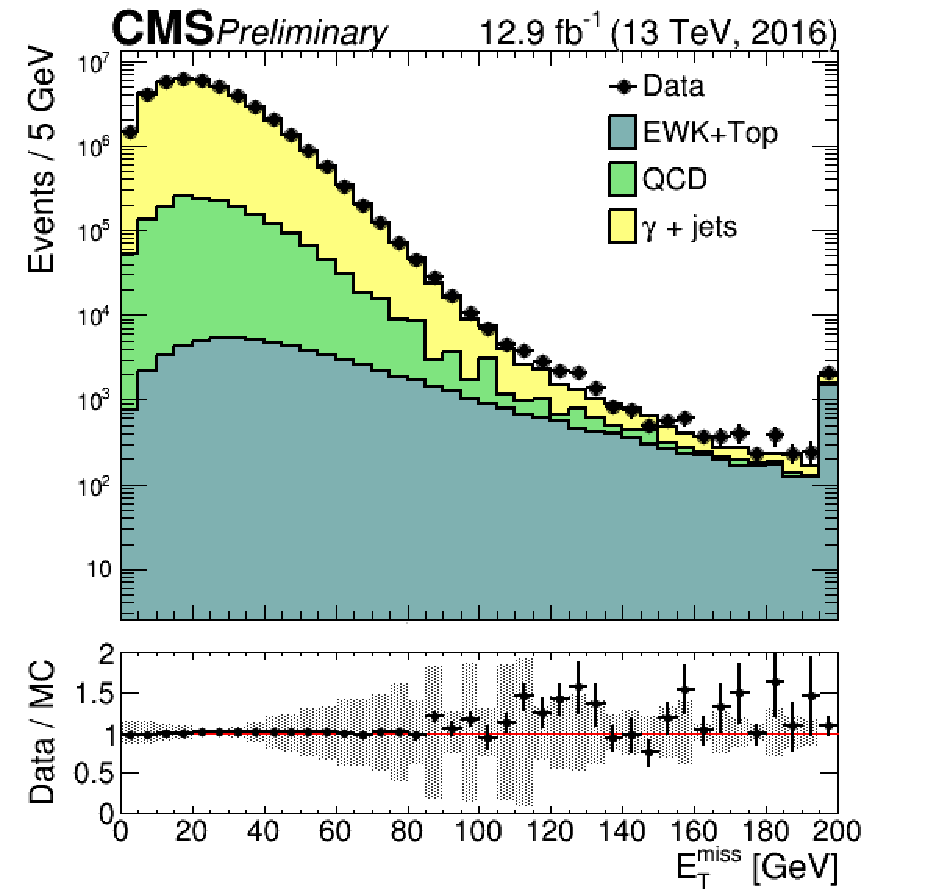
\includegraphics[width=.33\textwidth]{figures/MetPlots/distr_gamma.pdf}

%    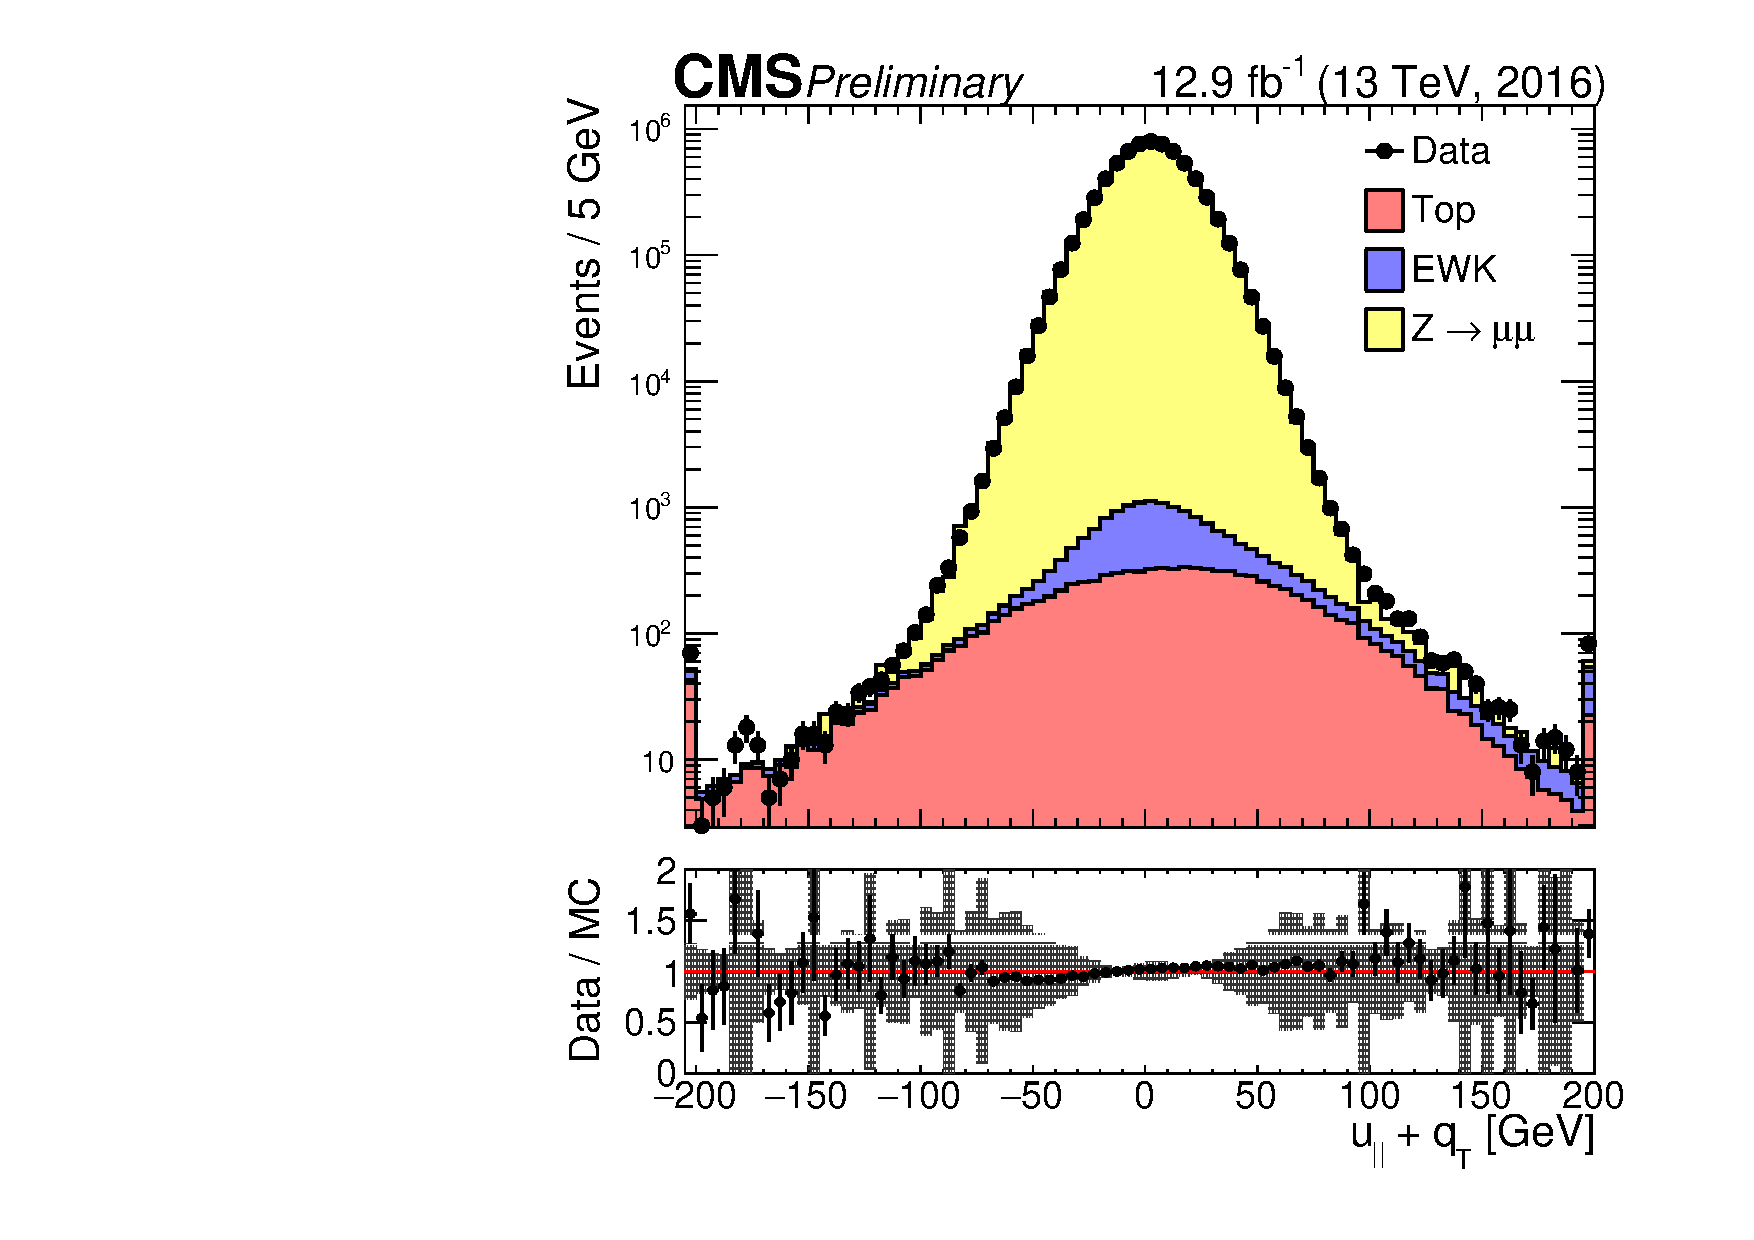
\includegraphics[width=.33\textwidth]{figures/MetPlots/u_para_mu.pdf}%
%    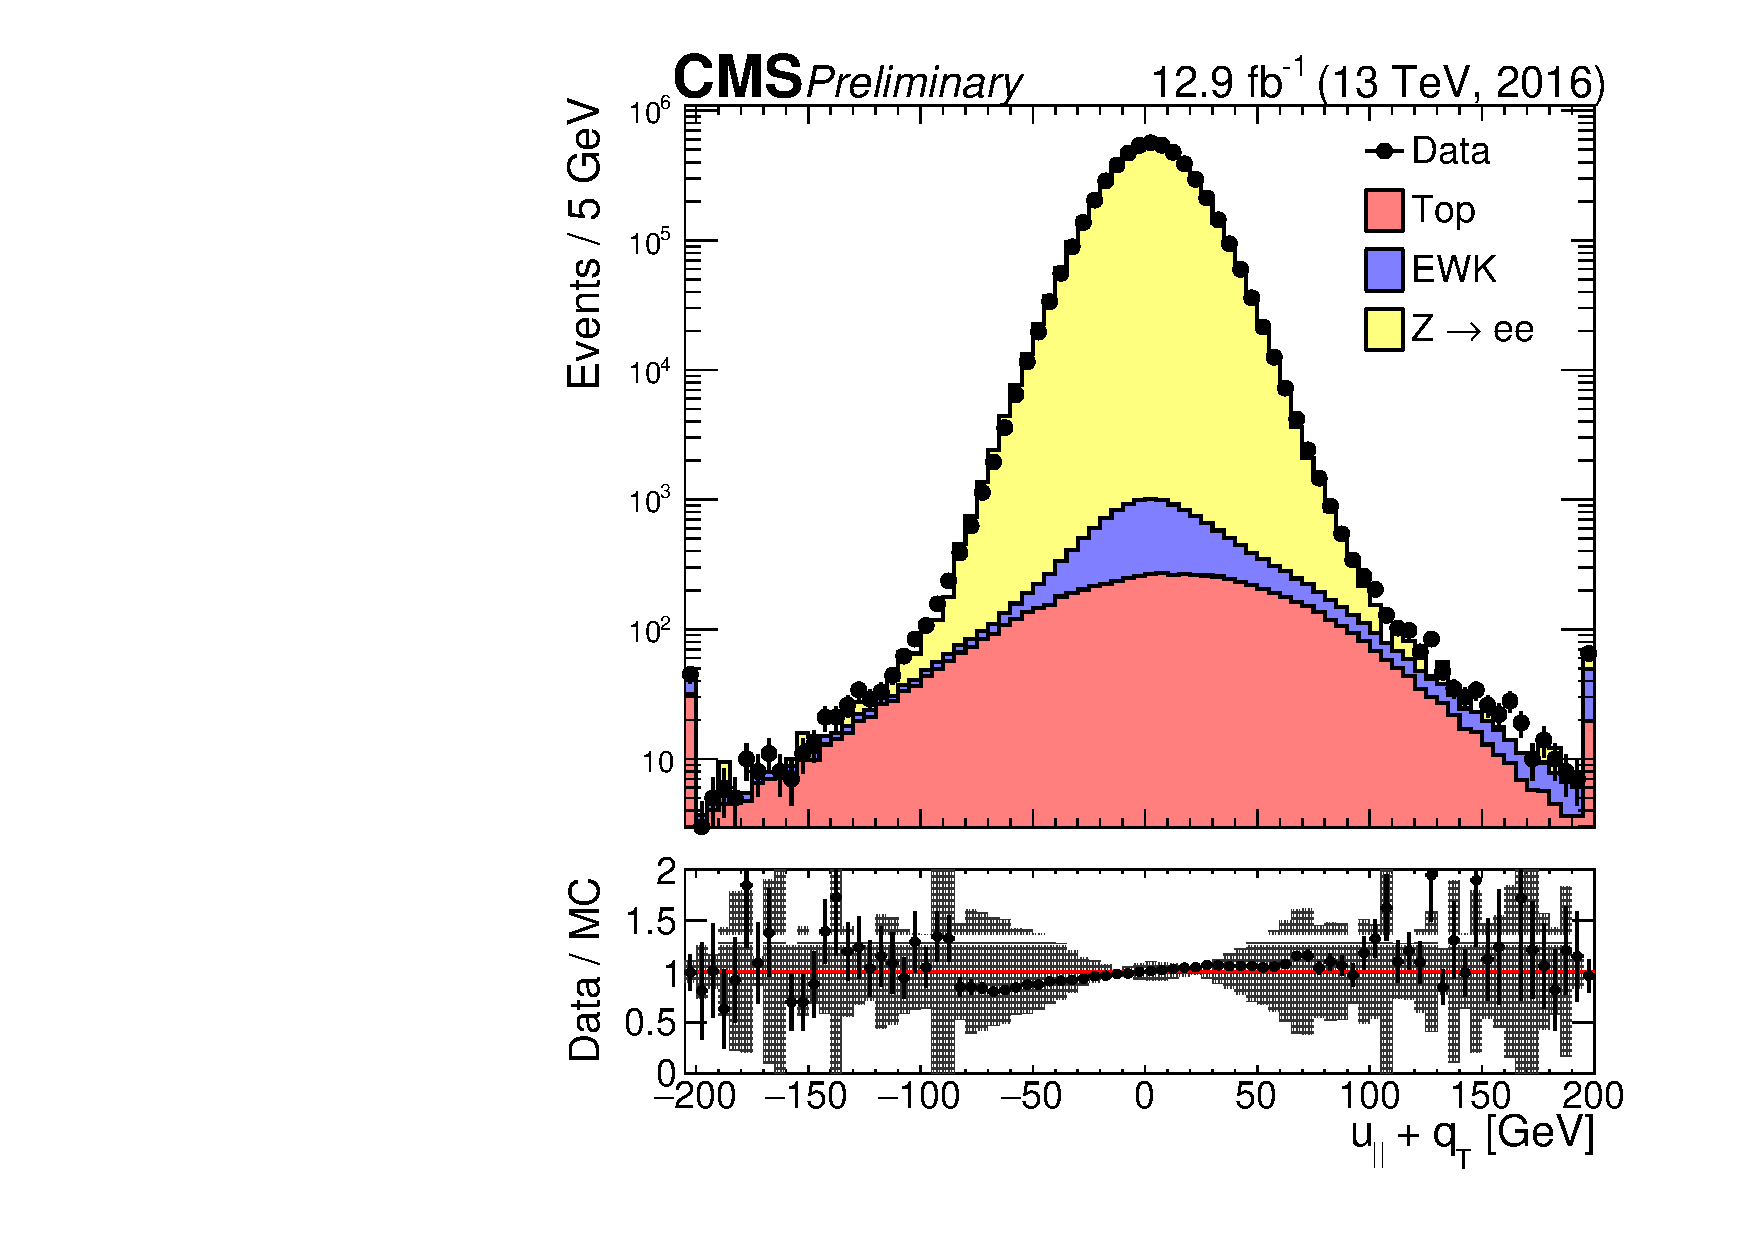
\includegraphics[width=.33\textwidth]{figures/MetPlots/u_para_ele.pdf}%
%    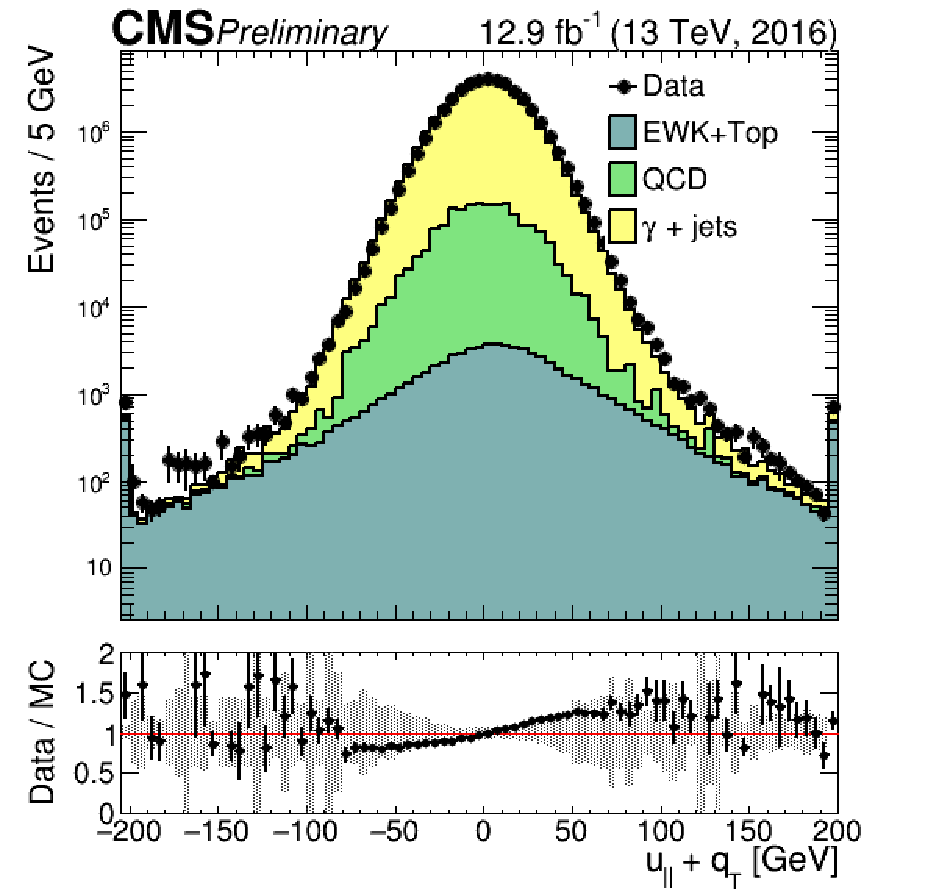
\includegraphics[width=.33\textwidth]{figures/MetPlots/u_para_gamma.pdf}

%    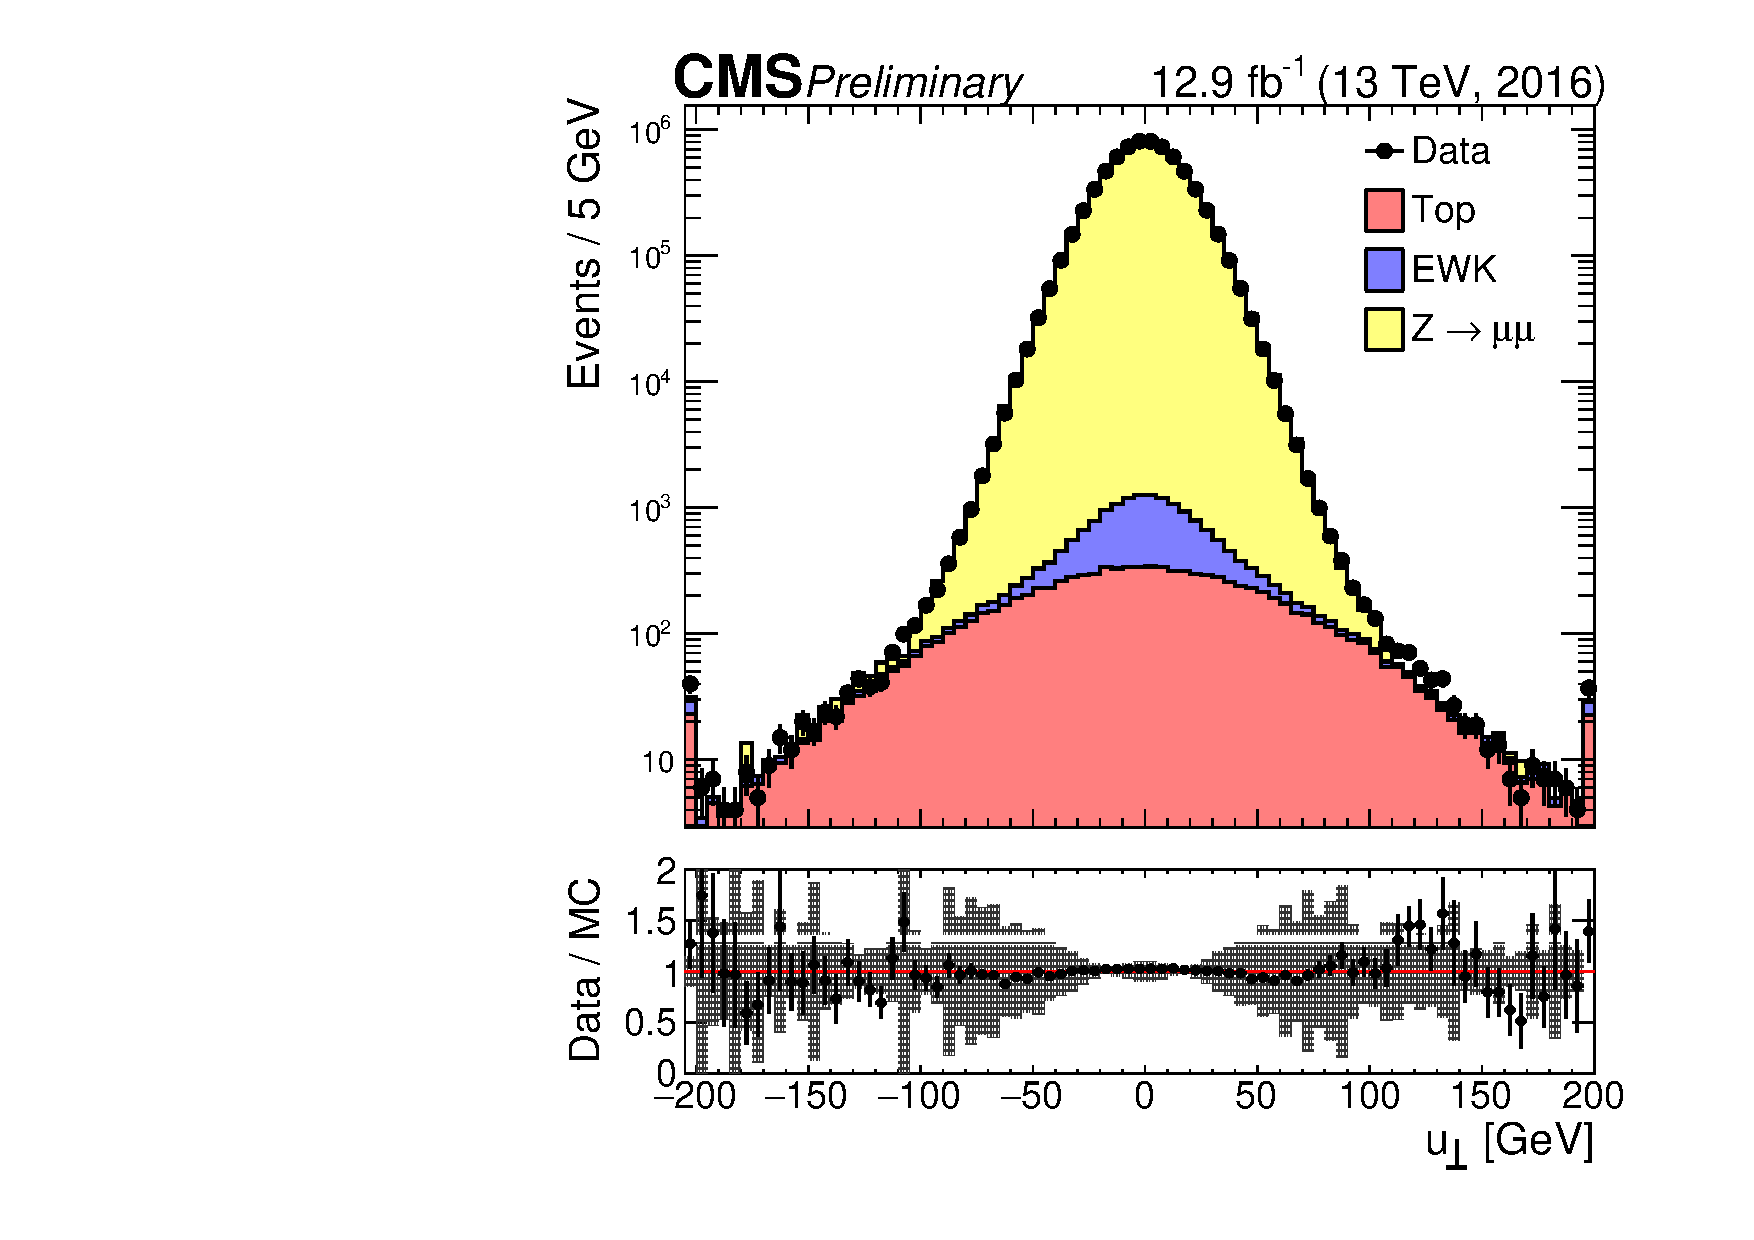
\includegraphics[width=.33\textwidth]{figures/MetPlots/u_perp_mu.pdf}%
%    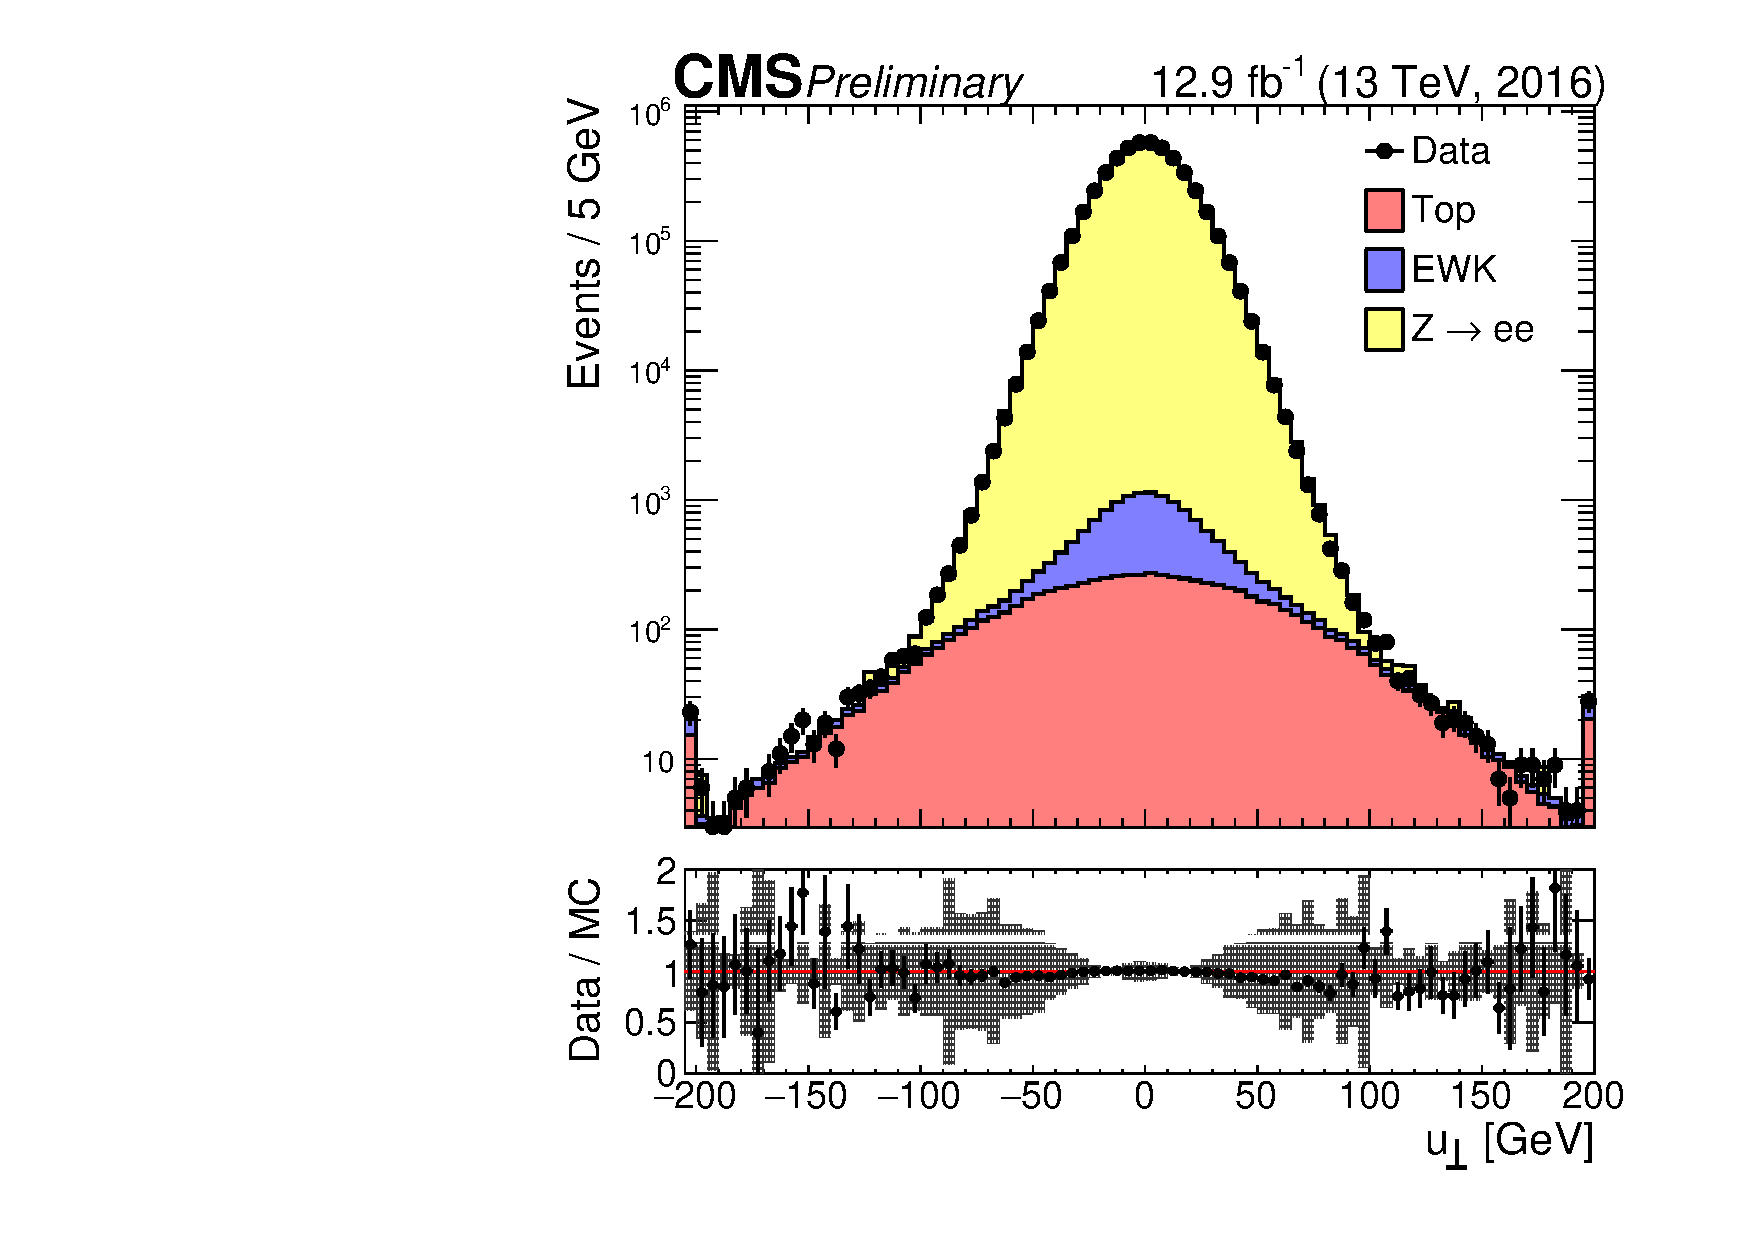
\includegraphics[width=.33\textwidth]{figures/MetPlots/u_perp_ele.pdf}%
%    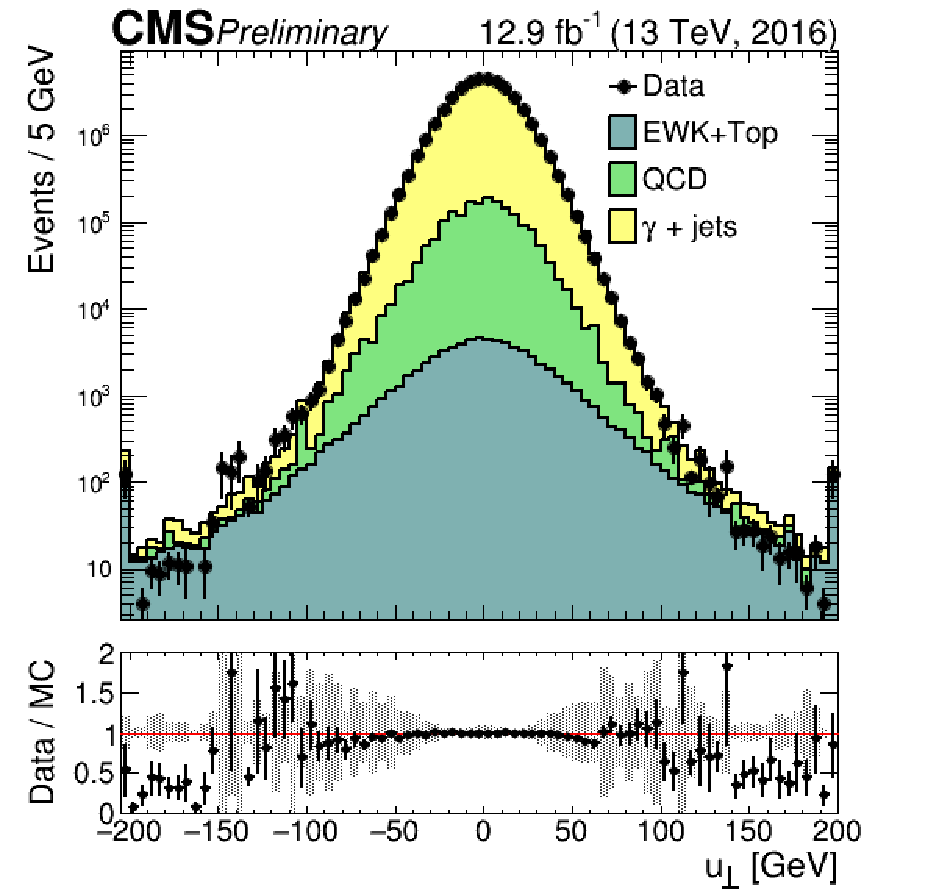
\includegraphics[width=.33\textwidth]{figures/MetPlots/u_perp_gamma.pdf}
  \caption{Data (black markers) and Monte Carlo (histograms) distributions of \MET variable, in events reconstructing respectively a $Z \rightarrow \mu \mu$ decay (left), a $Z \rightarrow e e$ decay (center), an isolated photon (right).}
  \label{fig:recoil_distribution}
\end{figure}

\noindent The hadronic recoil is projected in the parallel and perpendicular directions with regards to $\vec{q}_T$. The components $u_{\parallel}$ and $u_{\bot}$, along with the vectors described in eq.\ref{eq:recoil_def}, are schematically represented in fig.~\ref{fig:recoil}. The \MET response, defined as $- \langle u_{\parallel} \rangle / \langle q_T \rangle$, is calculated as a function of $q_T$ in data and simulations (fig.~\ref{fig:met_response}, left). The distributions of the two components of the hadronic recoil, $u_{\parallel} + q_T$ and $u_{\bot}$, are modelled as Voigtian functions (the convolution of a Gaussian with a Breit-Wigner). %, and are shown in fig.~\ref{fig:recoil_distribution} (central and bottom row), for each data sample ($Z \rightarrow \mu \mu$, $Z \rightarrow e e$, $\gamma$).
 The resolution of each component is calculated as the full width at half maximum of the corresponding Voigtian, and it is displayed in fig.~\ref{fig:met_response} (center and right plots), as a function of $q_T$.

\begin{figure}[!htb]
  \centering
    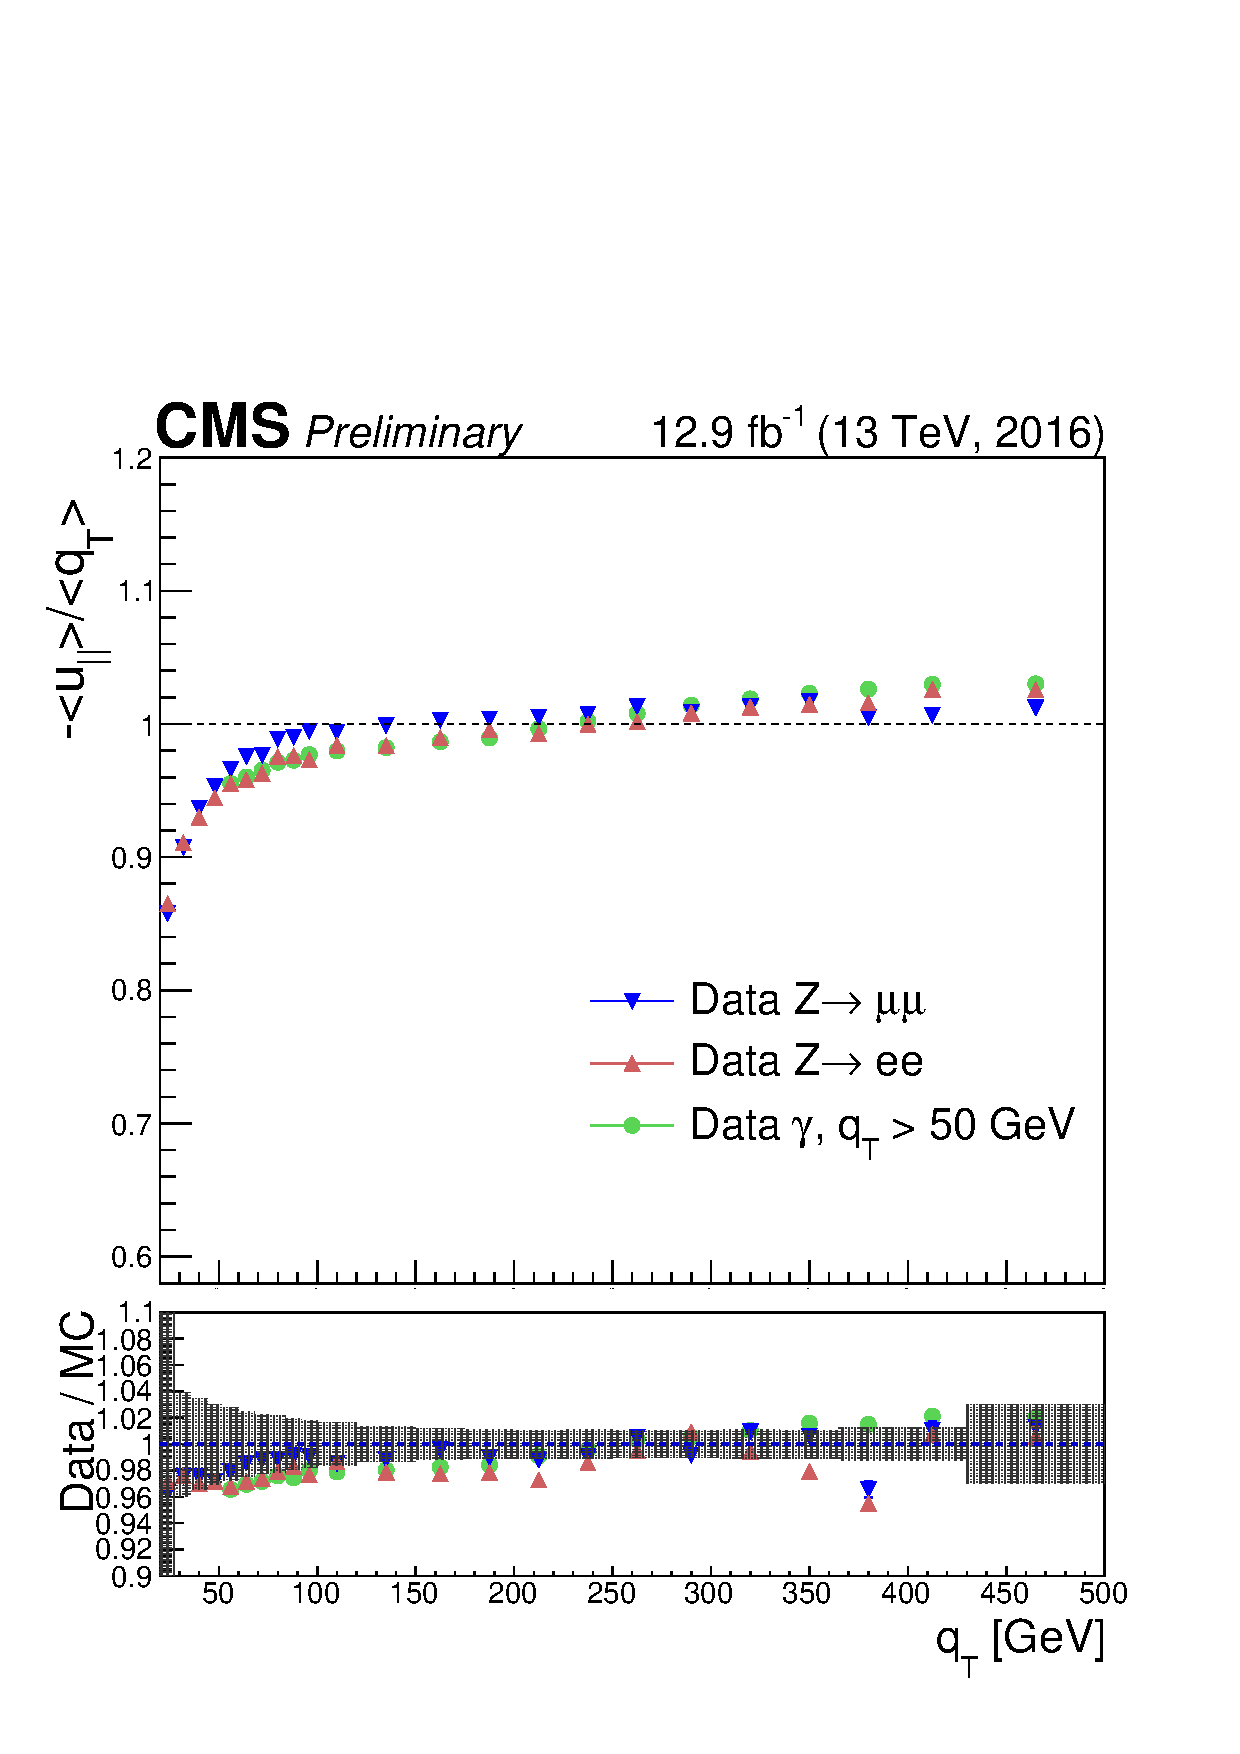
\includegraphics[width=.33\textwidth]{figures/MetPlots/response.pdf}%
    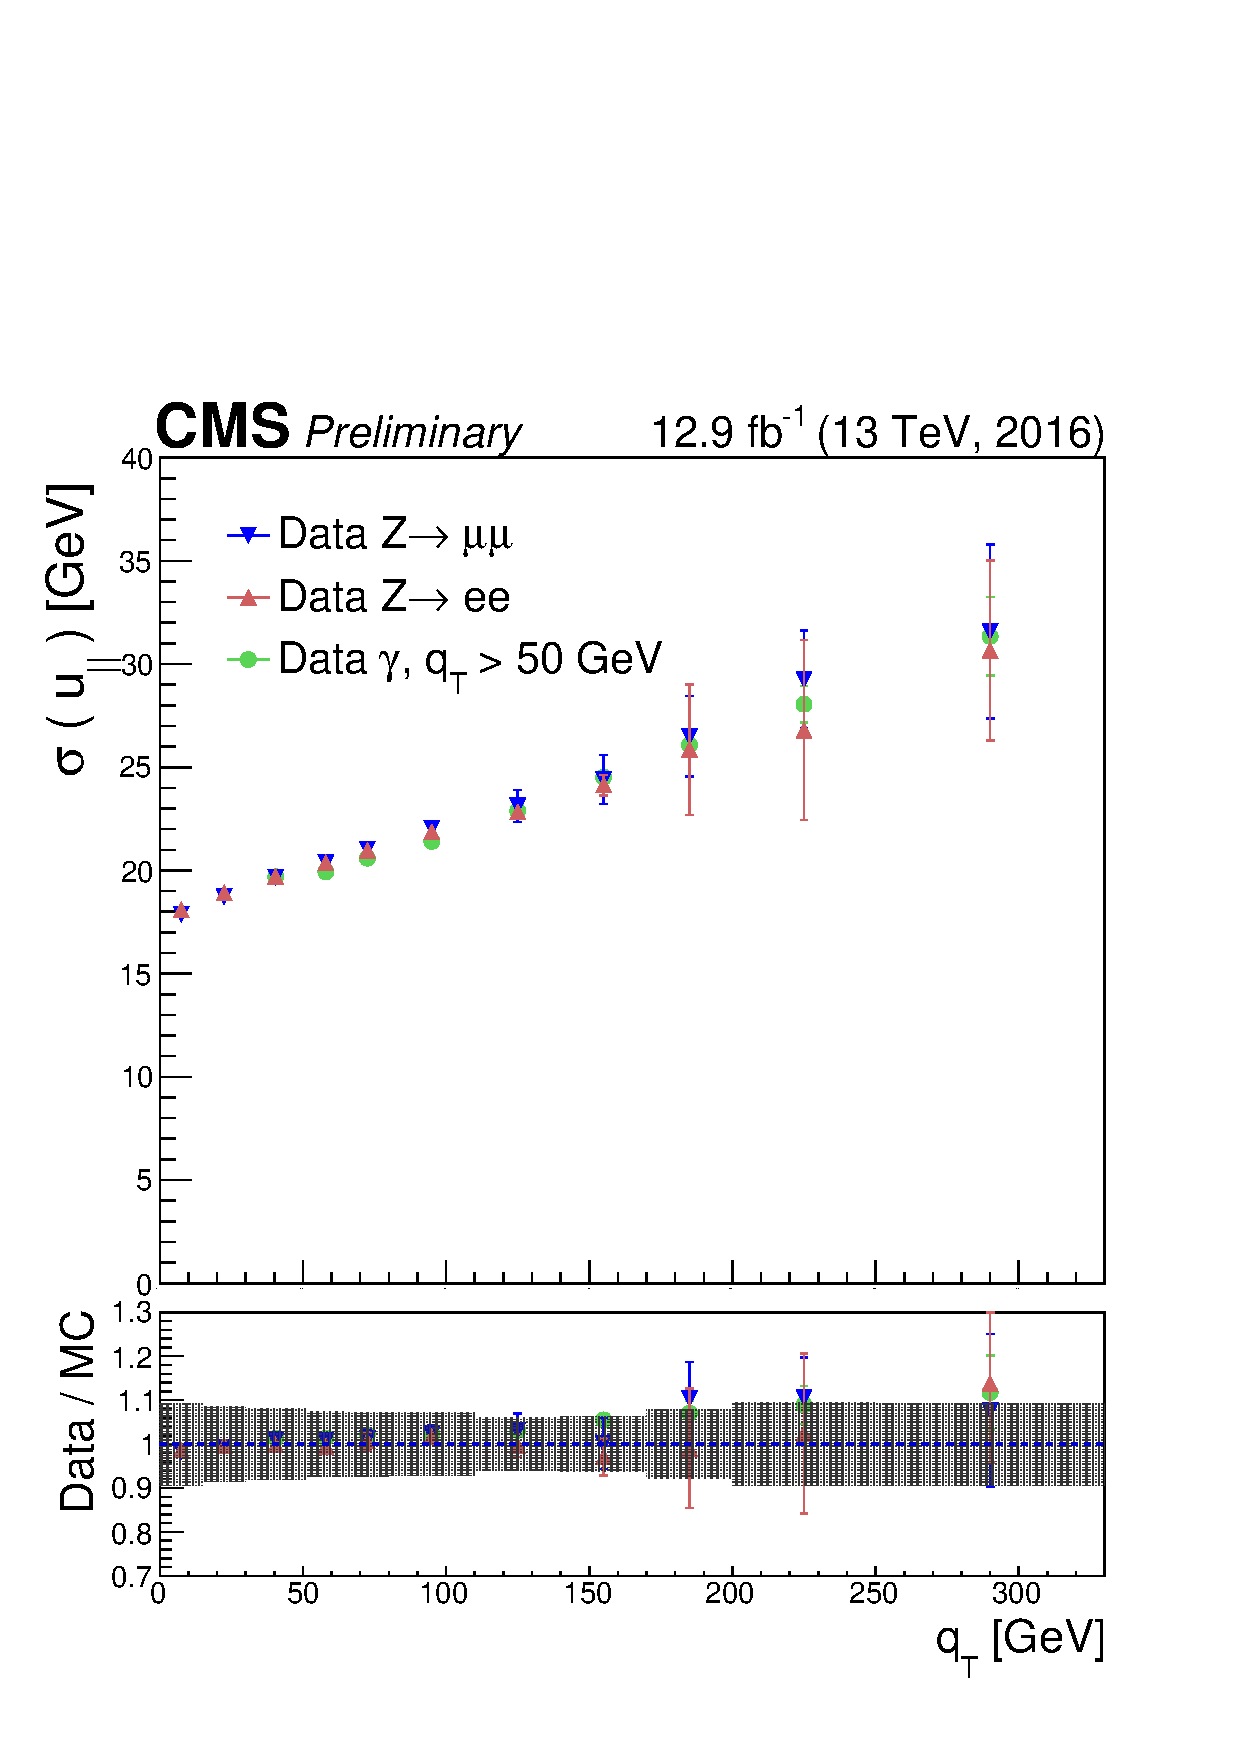
\includegraphics[width=.33\textwidth]{figures/MetPlots/u_para_res.pdf}%
    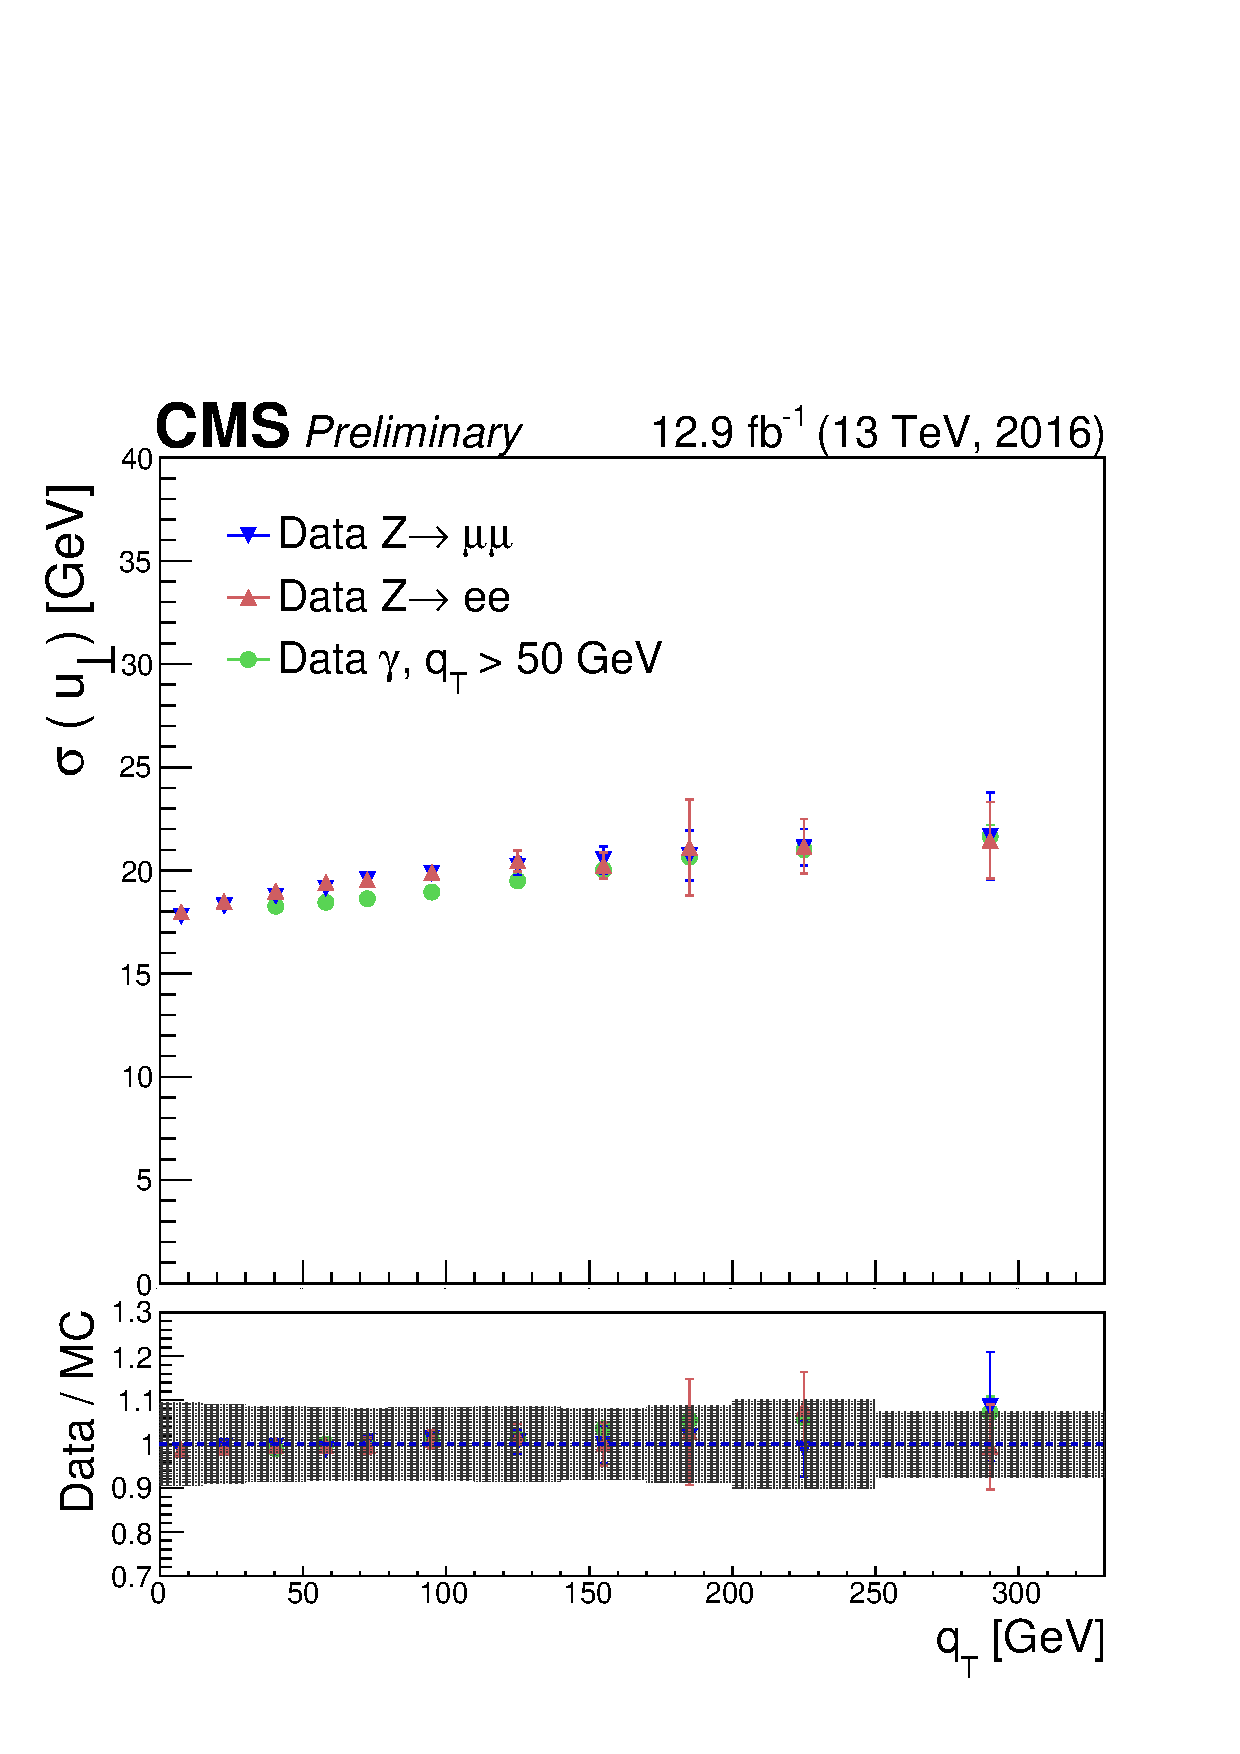
\includegraphics[width=.33\textwidth]{figures/MetPlots/u_perp_res.pdf}

  \caption{Left: \MET response, as a function of the transverse momentum $q_T$ of the vector boson considered in the event (Z decaying in $\mu \mu$, Z in $ee$ or a photon), measured on data. Center and right: resolution on the measurement of the parallel and perpendicular hadronic recoil in data, as a function of $q_T$.}
  \label{fig:met_response}
\end{figure}

%\noindent Distribution in fig... The data distributions are modeled well by the simulation. The increase in the uncertainty band in Fig. 6 around 60  GeV is due to the large impact of the unclustered energy uncertainties.

%%%%%%%%%%%%%%%%%%%%%%%%%%%%%%%%%%%%%%%%%%%%%%%%%%%%%%%
%Things I didn't understand:

%1% The back-to-back nature of events implies that u‖ is balanced with qT, thus centering u‖ + qT around zero. The u⊥ distribution is found to be symmetric because of the isotropic nature of energy fluctuations due to detector noise and underlying event.

%2% The curves show that the EmissT is able to fully recover the hadronic recoil activity corresponding to a Z boson qT of 50 GeV, whereas below that, the uncorrected unclustered energy contributions are dominating compared to the corrected energy of the recoiling jets.  The response in data and simulation is in agreement well within the uncertainties.

%3% The resolutions measured in the different samples are in good agreement and are found to be increasing with the qT. The isotropic nature of energy fluctuations, such as detector noise and underlying event, causes the perpendicular component of the recoil energy to have a more stable resolution compared to the parallel component.

%\clearpage
\section{ATLAS, ALICE, LHCb detectors}

\subsection{ATLAS}
ATLAS (A Toroidal LHC ApparatuS)~\cite{Aad:2008zzm} is a multi-purpose experiment, that shares the same scientifical aims of CMS. The simultaneous observation of an Higgs boson-like particle at the two experimental facilities represented an irrefutable proof of the discovery of the Higgs boson.\\
ATLAS has a cylindrical shape (diameter of 25 m, length of 46 m) and weights 7000 tons. Like CMS, ATLAS is composed by many sub-detectors: trackers, calorimeters and muon system. The ATLAS magnetic field is provided by a solenoid, located inside the cylinder, and a big toroid, located outside the sub-detectors, able to reach a magnetic field of 2 T at the interaction point. The main differences among the two experiments are listed below.

\begin{itemize}
\item {\itshape Tracker --} the CMS tracker has a better $p_T$ resolution (mainly due to the higher magnetic field): $\sigma_{p_T}/p_T \approx 5 \cdot 10^{-4} p_T + 0.01$ at ATLAS; $\sigma_{p_T}/p_T \approx 1.5 \cdot 10^{-4} p_T + 0.005$ at CMS.
\item {\itshape Electromagnetic calorimeter --} the CMS electromagnetic calorimeter is completely enclosed inside the solenoid, whilst ATLAS calorimeter is outside of the solenoid. The particles going through the solenoid suffer an energy loss and a consequent deterioration of the energy resolution. The CMS ECAL has an energy resolution of $\sigma_E /E \approx 3\%/\sqrt{E}$; the ATLAS calorimeter has a sandwich structure (liquid argon and lead layers) and a resolution of $\sigma_E / E \approx 10\%/\sqrt{E}$.
\item {\itshape Hadronic calorimeter --} the CMS HCAL is partly inside the solenoid, partly outside, depauperating the resolution. The ATLAS hadronic calorimeter (made of iron and plastic scintillator tiles) has an energy resolution $\sigma_E /E \approx 50\%/\sqrt{E} + 0.03$ GeV; CMS HCAL has a resolution of $\sigma_E /E \approx 100\%/\sqrt{E} + 0.05$ GeV.
\item {\itshape Muon system --} the peculiar geometry of the ATLAS muon system allows a better resolution of the standalone measurement of the muon momenta (\textit{i.e.}, without using tracker and calorimeters), that is around 10\% at 1 TeV. CMS has better performance when combining the informations coming from the inner detectors (7\% at 1 TeV against the 35\% for the standalone measurement).
\end{itemize}

\subsection{ALICE}
ALICE (A Large Ion Collider Experiment)~\cite{Aamodt:2008zz} studies the heavy ion collisions (lead-lead) or proton-ion in order to explore the physics of the hadrons in high density (or temperature) regimes, when a new state of matter appears, the so-called quark-gluon plasma (QGP). The QGP played a crucial role in the very first instants of the life of the universe.

\subsection{LHCb}
LHCb (Large Hadron Collider beauty)~\cite{Alves:2008zz} is a detector designed to study the b-quark properties, in particular the CP violation and other rare phenomena related to B hadrons. The final aim of these measurements is trying to solve the matter-antimatter asymmetry problem.

\vspace*{1\baselineskip}

\noindent The three detectors are depicted in fig.~\ref{fig:ATLAS-ALICE-LHCb}.%{fig:ATLAS}--\ref{fig:LHCb}.


\begin{figure}%{l}{0.5\textwidth}
\centering
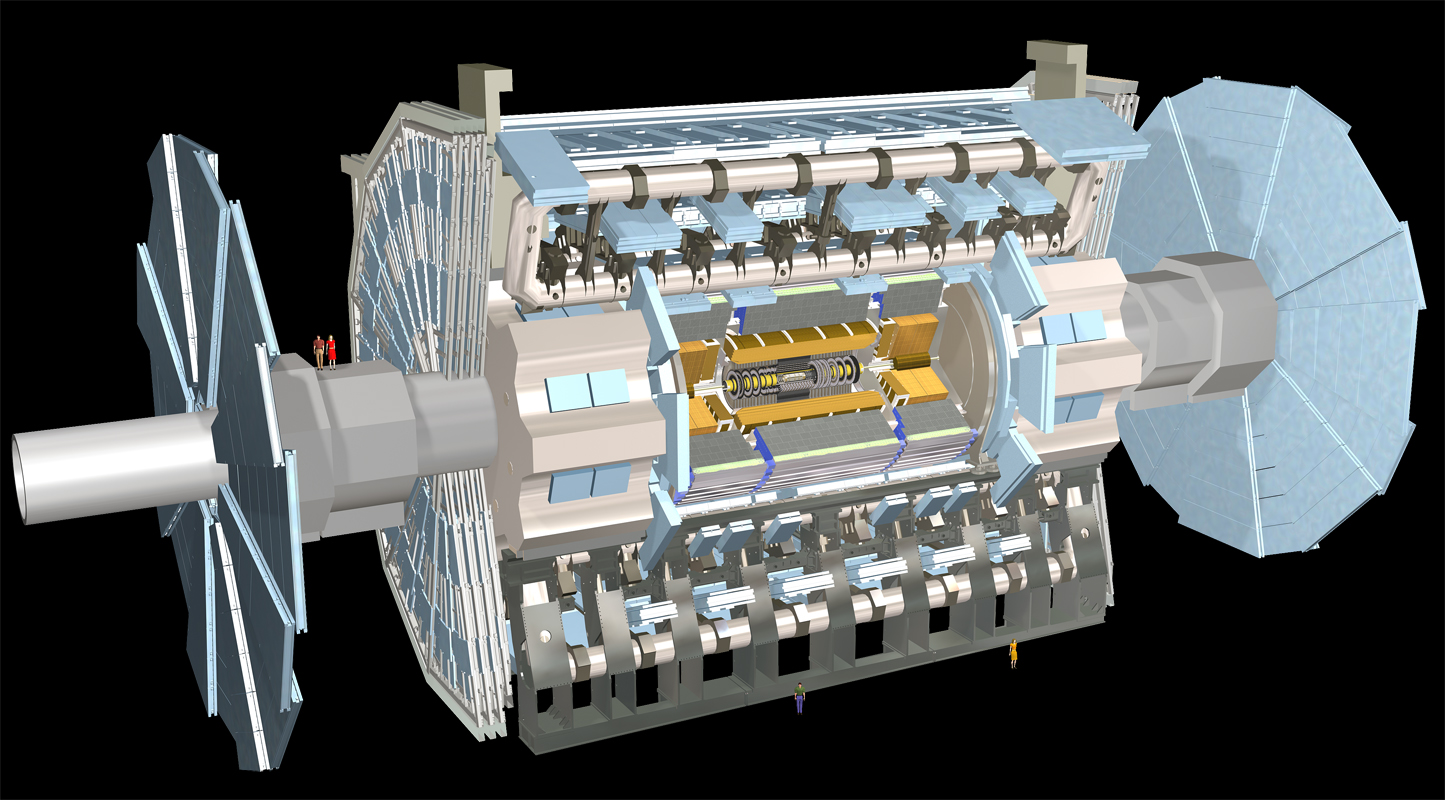
\includegraphics[width=.65\textwidth]{figures/ATLAS.jpg}
%\caption{The ATLAS experiment.}
%\label{fig:ATLAS}
%\end{figure}

%\begin{figure}%{l}{0.5\textwidth}
%\centering
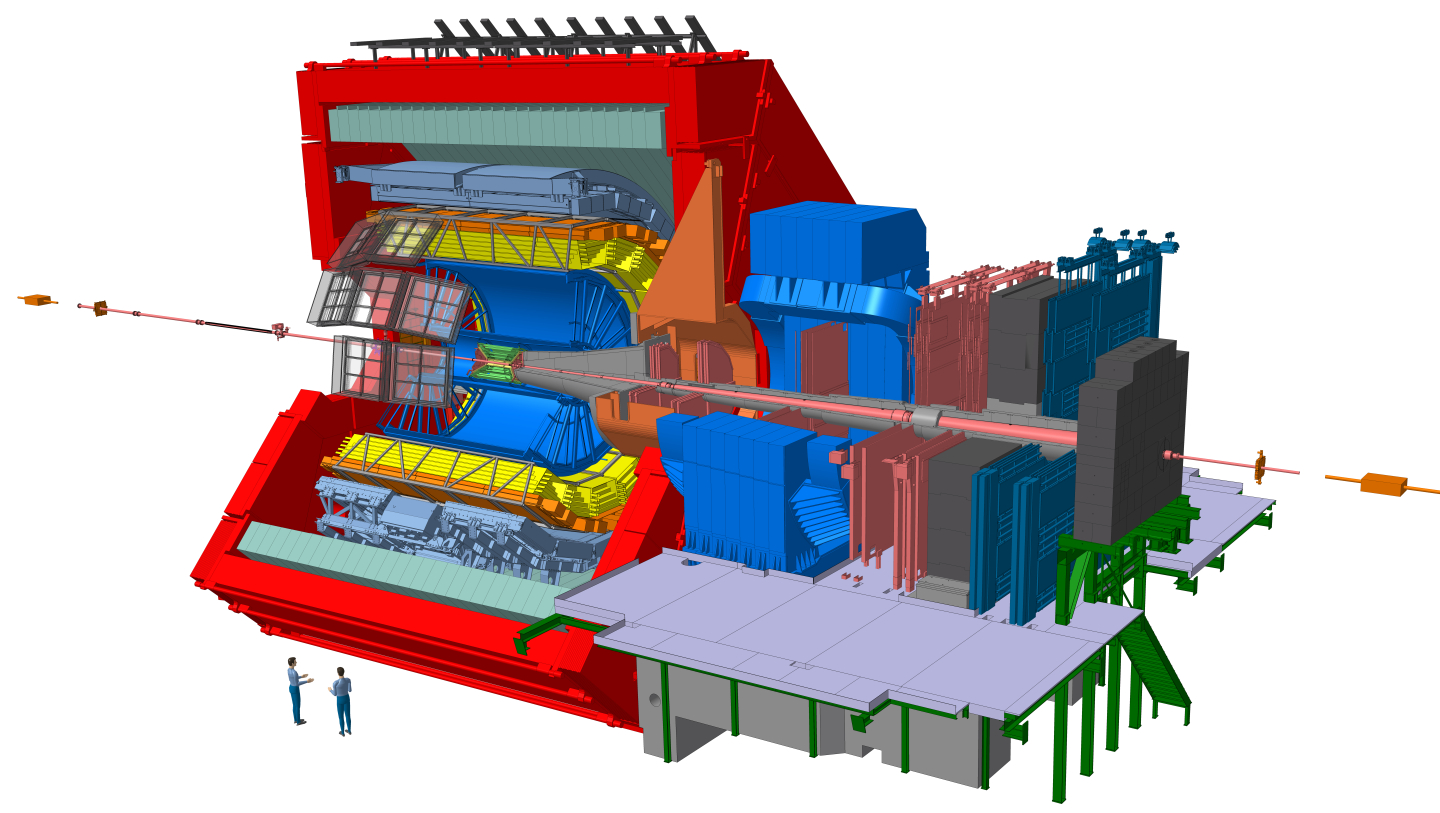
\includegraphics[width=.65\textwidth]{figures/ALICE.jpg}
%\caption{The ALICE experiment.}
%\label{fig:ALICE}
%\end{figure}

%\begin{figure}%{l}{0.5\textwidth}
%\centering
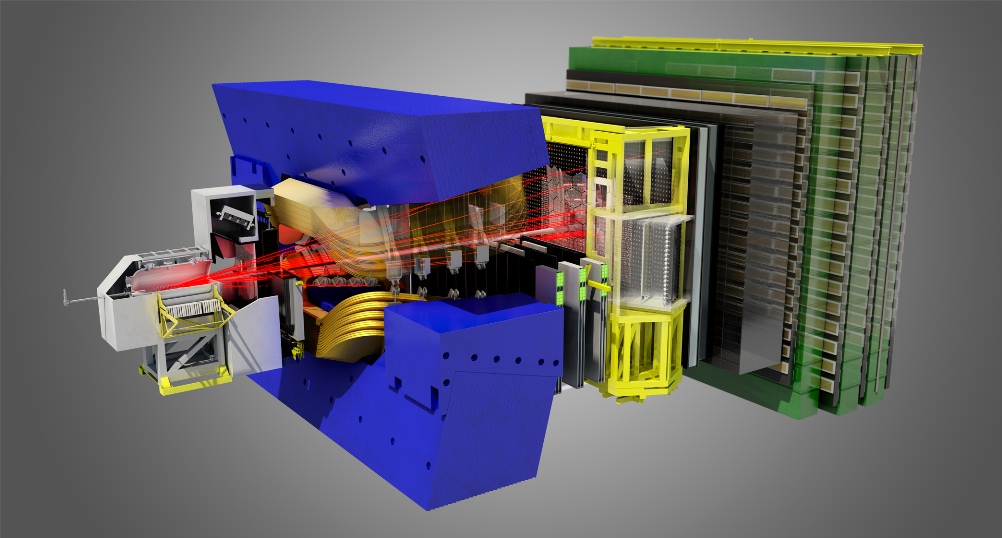
\includegraphics[width=.65\textwidth]{figures/LHCb.png}
%\caption{The LHCb experiment.}
%\label{fig:LHCb}
%\end{figure}

\caption{Top: the ATLAS experiment. Center: the ALICE experiment. Bottom: the LHCb experiment.}
\label{fig:ATLAS-ALICE-LHCb}
\end{figure}

\clearpage
